\chapter{Search for heavy scalars and pseudoscalars in \ttbartitle}
\label{ch:ah}

\section{Introduction}
\label{sec:ah:intro}

As explained in \cref{sec:theory:hext}, additional spin-0 particles are predicted in many attractive extensions of the Standard Model, and searches for such particles at the LHC have potential of discovering hints for new physics. Oftentimes, such models predict Yukawa-type couplings for the new particles to SM fermions, which scale with the fermion mass. It is thus natural to search for interactions of new spin-0 states with the heaviest fundamental particle in the SM: the top quark.

In particular, if the mass of any such new state is larger than double the top quark mass, it can decay to a \ttbar final state. This decay channel will be dominant in many scenarios. If the new state is produced in gluon fusion, the resulting process will interfere with SM \ttbar production as discussed in \cref{sec:theory:ttbar}, leading to an interference pattern in the invariant \ttbar mass that can be probed experimentally.

To do so, a generic model describing the new particles is defined, containing two new spin-0 states A and H which both couple solely to the top quark via a pseudoscalar (for A) and a scalar (for H) Yukawa interaction. The Lagrangian reads

\begin{equation}
\label{eq:ah:lagrangian}
\begin{split}
    \mathcal{L}_{\AH} =& \, \frac{1}{2} (\partial_\mu A ) (\partial^\mu A ) +\frac{\mA^2}{2} A^2  
    + i  \gAtt \, \frac{\mt}{v} \bar t  \gamma_5 \, t  \, A \\
    & + \frac{1}{2} (\partial_\mu H ) (\partial^\mu H ) +\frac{\mH^2}{2} H^2  
    -  \gHtt \, \frac{\mt}{v} \bar t \, t  \, H \,
\end{split}
\end{equation}

Here, \mA and \mH are the masses of the new particles, \gAtt and \gHtt are the coupling modifiers for the top quark Yukawa couplings, \mt is the top quark mass, and $v$ is the vacuum expectation value of the SM Higgs boson. 

This model assumes that the two states A and H do not mix, which is equivalent to the assumption that there is no CP violation [??]. Apart from this assumption, it is fully generic and can be mapped onto any of the models discussed in \cref{sec:theory:hext}, provided that only couplings to the top quark are considered. This makes it ideal for an experimental search, as results presented using this model can be easily reinterpreted in various models of interest.

In addition to the masses and coupling modifiers, the decay widths \wA and \wH of the two particles are also considered as free parameters, yielding six free parameters total. This is because, due to interactions with other SM particles besides the top quark, or with additional BSM particles, concrete models (e.g. the 2HDM) will predict different decay widths then the natural width expected in the simplified model. In particular, if either or both of the particles is to be considered a dark matter mediator, it will have a significant branching ratio to dark matter particles, increasing its absolute width.

This chapter presents a search for new spin-0 states with either scalar or pseudoscalar interactions with the top quark, using the full Run~2 dataset ($L= \SI{138}{\fbinv}$). The work done as part of this thesis focused on the dilepton decay channel of \ttbar, which is thus described in detail in~\cref{sec:ah:setup,sec:ah:ttbarweights,sec:ah:mereweighting,sec:ah:prefit}. It was then combined with a similar analysis of the \ljets decay channel, and the results of both the dilepton channel alone and the combination are discussed in \cref{sec:ah:etat,sec:ah:limits}.

\section{Analysis setup}
\label{sec:ah:setup}

\subsection{Datasets}
\label{sec:ah:datasets}

\paragraph{Experimental data.} 
The analysis is performed using the full CMS Run~2 ultra-legacy (UL) dataset, which is the final, re-reconstructed and recalibrated dataset recommended by CMS for physics analyses. It is split into the three datataking years of Run~2: 2016, 2017 and 2018, where 2016 is again split into two parts, denoted as "2016pre" and "2016post". \todo{why is 2016 split} 

A similar combination of dilepton and single-lepton triggers as in \cref{sec:ttxs:datasets} is used for all years, with the \pt thresholds varying slightly between datataking eras, as shown in \cref{tab:ah:triggers}. 

\begin{table}
\centering
\begin{tabular}{|c|c|c|}
    \hline
    Trigger & Year & Lepton \pt requirement \\
    \hline
    \multirowcell{3}{single-e} & 2016 & $e(\pt > \SI{27}{\GeV})$ \\
    & 2017 & $e(\pt > \SI{35}{\GeV})$ \\
    & 2018 & $e(\pt > \SI{32}{\GeV})$ \\
    \hline
    \multirowcell{3}{single-$\mu$} & 2016 & $\mu(\pt > \SI{24}{\GeV})$ \\
    & 2017 & $\mu(\pt > \SI{27}{\GeV})$ \\
    & 2018 & $\mu(\pt > \SI{24}{\GeV})$ \\
    \hline
    \multirowcell{2}{e$\mu$} & \multirowcell{2}{all} & $e(\pt > \SI{12}{\GeV})$ and $\mu(\pt > \SI{23}{\GeV})$ or \\
    & & $e(\pt > \SI{23}{\GeV})$ and $\mu(\pt > \SI{8}{\GeV})$ \\
    \hline
    ee & all & $e_1(\pt > \SI{23}{\GeV})$ and $e_2(\pt > \SI{12}{\GeV})$ \\
    \hline
    $\mu \mu$ & all & $\mu_1(\pt > \SI{17}{\GeV})$ and $\mu_2(\pt > \SI{8}{\GeV})$ \\
    \hline
\end{tabular}
\caption{\textbf{Trigger \pt thresholds.} Overview of the used triggers in the three datataking years, as well as their lepton \pt thresholds.}
\label{tab:ah:triggers}
\end{table}

\paragraph{Background simulation.}
Since this analysis is, in essence, a search for interference patterns of the signal with the SM \ttbar background, it is clear that a large irreducible background is expected. As a result, it is essential that the SM Monte Carlo simulation is as both theoretically precise and has sufficient statistics, and that any remaining imprecisions are covered by the systematic uncertainty model.

The SM \ttbar background is again simulated at NLO in QCD with the \texttt{hvq} process from the  MC generator package \powhegvtwo and interfaced to \textsc{Pythia 8} for showering. Similar settings as in \cref{sec:ttxs:datasets} have been used. To achieve the necessary precision, the NLO simulation is reweighted to higher orders in both QCD and electroweak (EW) processes, which is described in \cref{sec:ah:ttbarweights}.

In addition, several minor backgrounds are included, a summary of which can be found in \cref{tab:ah:simulation}. Of note here is the Z+jets background, which is simulated at NNLO in QCD using the MiNNLO method in \powhegvtwo. It was found here that the higher-order corrections are relevant to the analysis especially for low values of the invariant dilepton mass \mll. Most processes are normalized to cross sections predicted at higher orders of QCD where available, which can be found in \cref{tab:ah:crosssections}.

\begin{table}
\centering
\begin{tabular}{|c|c|c|}
    \hline
     Process & QCD order & ME Generator \\
     \hline
     \ttbar & NLO & \powhegvtwo (\texttt{hvq}) \\
     tW & NLO & \powhegvtwo (\texttt{ST\_wtch}) \\
     \Zgamma+jets & NNLO & \powhegvtwo (\texttt{Zj} MiNNLO) \\
     $t$-channel single top & NLO & \powhegvtwo (\texttt{ST\_tch}) + \textsc{MadSpin} \\
     $s$-channel single top & NLO & \amcatnlo \\
     $\ttbar \mathrm{W}$ & NLO & \amcatnlo \\
     $\ttbar \mathrm{Z}$ & NLO & \amcatnlo \\
     WW, WZ \& ZZ & LO & \pythia 8.2 \\
     \hline
     \AH signal & LO & \amcatnlo \\
     \etat signal & LO & \amcatnlo \\
     \hline
\end{tabular}
\caption{\textbf{Simulated background and signal samples.} An overview of the different background and signal processes considered, as well as the theoretical order in QCD and the ME generator used to simulate them. For all samples, \textsc{Pythia 8.2} is used for showering and hadronization.}
\label{tab:ah:simulation}
\end{table}

\begin{table}
    \centering 
    \begin{tabular}{|c|c|c|c|}
        \hline
         Process & Cross section (pb) & Order & Program / reference \\
         \hline
         \ttbar & 833.9 & NNLO+NNLL & Top++~\cite{Czakon:2011xx} \\
         tW & 71.7 & NNLO (approx.) & \cite{Kidonakis:2021vob} \\
         $t$-channel single top & 217.0 & NLO & Hathor~\cite{Aliev:2010zk,Kant:2014oha} \\
         $s$-channel single top & 10.3 & NLO & Hathor~\cite{Aliev:2010zk,Kant:2014oha} \\
         $\ttbar \mathrm{W}$ & 0.64 & NLO & \amcatnlo \\
         $\ttbar \mathrm{Z}$ & 0.75 & NLO & \amcatnlo \\
         \Zgamma+jets & \multirowcell{2}{$24.7 \times 10^3$} & \multirowcell{2}{NNLO} & \multirowcell{2}{FEWZ~\cite{Melnikov:2006kv,Li:2012wna}}  \\
         $\Zgamma\rightarrow\ell\ell$, $\mll > \SI{10}{\GeV}$ & & & \\
         WW & 118.7 & NNLO & \cite{Gehrmann:2014fva} \\
         WZ & 471.3 & NLO & MCFM~\cite{Campbell:2010ff} \\
         ZZ & 165.2 & NLO & MCFM~\cite{Campbell:2010ff} \\
         \hline
    \end{tabular}
    \caption{\textbf{Cross sections for background processes.} The cross sections used for the normalization of background processes relevant for this search, as well as the orders in QCD at which they were computed.}
    \label{tab:ah:crosssections}
\end{table}

\paragraph{Signal simulation.}

The signal for the general \AH model described in \cref{sec:ah:intro} is generated at LO in QCD using \textsc{MadGraph 5} with a custom Universal FeynRules Output (UFO) model. The $p p \to \AH \to \ttbar$ resonance and the \AH-SM interference are simulated separately, and both are again showered with \textsc{Pythia 8}. In order to cover the phase space of the \AH model, the signals are generated for all combinations of the following values of the \AH masses and widths:

\begin{equation}
\begin{split}
    m_{\AH} &\in \{ 365, 400, 500, 600, 800, 1000 \} \, \si{\GeV} \\
    \Gamma_{\AH} / m_{\AH} &\in \{ 2.5, (5), 10, 25 \} \, \%
\end{split}
\end{equation}

Samples with a width of $5\%$ were generated only for masses of \SI{400}{\GeV}, which leads to 38 signal points total. In addition, samples for the pseudoscalar case only were generated with

\begin{equation}
    \mA \in \{ 450, 550, 700, 900 \} \, \si{GeV}, \quad \wA / \mA = 9 \, \%.
\end{equation}

All of these samples were combined and used reweighted at matrix element level to obtain also phase space points between these mass and width values, as described further in \cref{sec:ah:mereweighting}.

In order to probe possible non-perturbative effects in \ttbar, an additional signal sample is generated using the color-singlet \etat toy model described in \citere{Fuks:2021xje}, using a UFO model provided by the authors.

For all signal and background samples, the detector response is simulated with \textsc{Geant 4} and the full CMS simulation and reconstruction chain as described in [??] is performed.

\subsection{Object definition}
\label{sec:ah:objects}

\paragraph{Leptons.} 

All electrons and muons are required to have $\pt > \SI{20}{\GeV}$ and $\abseta < 2.4$ to be considered for the analysis. Similar to \cref{sec:ttxs:objects}, electrons in the transition region between barrel and endcaps in the ECAL are removed, and additional ID critera are applied for both types of leptons.

For electrons, the multivariate classifier (MVA)-based ID described in \citere{CMS:EGM-17-001} is used at a working point giving 90 \% background rejection. This ID already includes an isolation requirement as part of the MVA training, and no further requirement is applied.

For muons, the same cut-based ID from \citere{CMS:MUO-16-001} as in \cref{sec:ttxs:objects}, also at the tight working point, is used, and the same isolation requirement using a cone size of $\Delta R < 0.4$ is applied in addition.

\paragraph{Jets.} 

Jets are again reconstructed using the anti-$k_T$ algorithm~\cite{Cacciari:2008gp} with a distance parameter of $0.4$. They are required to fulfill $\pt > \SI{20}{\GeV}$, $\abseta < 2.4$, and have a minimum distance of $\Delta R > 0.4$ from all leptons passing the above criteria in the event.

The \textsc{DeepJet} algorithm~\cite{DeepJet:2020}, same as in \cref{sec:ttxs:objects}, is used to identify jets originating from the showering and hadronization of b quarks. The medium working point of \textsc{DeepJet} in CMS, corresponding to an identification efficiency of XX \% is chosen~\cite{CMS:BTV-16-002}.

\paragraph{Missing transverse momentum.}

In the dileptonic decay of \ttbar, the two neutrinos can not be measured experimentally, and escape the detector unseen. However, their presence can be inferred from momentum conservation: In a proton-proton collision, the longitudinal component of the incoming partons in the hard scattering process is unknown, while the transverse component can be assumed to be close to zero. Thus, the missing transverse momentum \ptmissvec can be inferred as the negative vectorial sum of all reconstructed objects (jets, leptons and photons)~\cite{CMS:JME-17-001}. Along with the leptons and jets, it will be used to reconstruct the \ttbar system.

\subsection{Event selection}

Events are selected with exactly two leptons of opposite electric charge and sorted into three channels (\ee, \emu and \mumu) by lepton flavor, similar to \cref{sec:ttxs:channels}. The two leptons need to fulfill $\pt > \SI{25}{\GeV}$ and $\pt < \SI{20}{\GeV}$ for the leading and subleading lepton, respectively, and their invariant mass is required to be $\mll > \SI{20}{\GeV}$ in order to reject background from $\gamma^*$+jets production and low-mass resonances. 

In all channels, at least two jets with $\pt > \SI{30}{\GeV}$ are required, of which at least one needs to be b-tagged. Furthermore, in the same-flavor lepton channels (\ee and \mumu), additional cuts are applied to reject Z+jets background: Events with $|\mll - m_Z| < \SI{15}{\GeV}$, i.e. close to the Z boson mass peak, are discarded (again just as in \cref{sec:ttxs:channels}), and the magnitude of the missing transverse momentum is required to be $\ptmiss > \SI{40}{\GeV}$.

The effect of all selection cuts can be seen in \cref{fig:ah:cutflows}.

\begin{figure}[h]
    \centering
    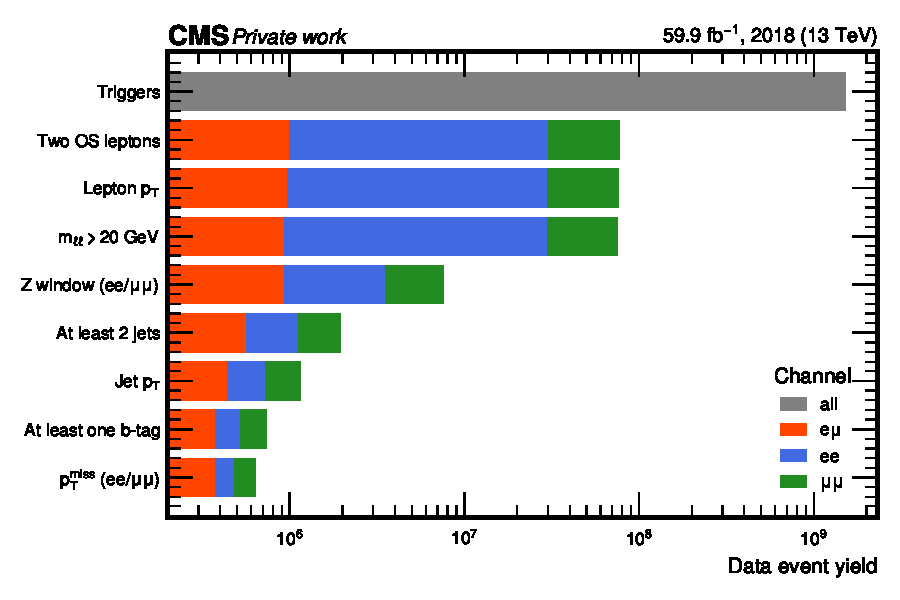
\includegraphics[width=\textwidth]{figures/ah/cutflows.pdf}
    \caption{\textbf{Selection cuts.} Shown is the data yield in 2018 (corresponding to $\Lint = \lumiVIII$) after successively applying all selection cuts. Starting with the requirement of two opposite-sign leptons, the three channels are marked with different colors.}
    \label{fig:ah:cutflows}
\end{figure}

\subsection{Experimental corrections}

Similar as in \cref{sec:ttxs:corrections}, several corrections are applied to the MC simulation in order to achieve good agreement with the data. In contrast to the \ttbar cross section measurement, where most of these corrections were derived as part of this work, many of the experimental corrections used in this chapter were provided centrally by the CMS collaboration. These will only be described very briefly; more details can be found in the associated references.

\paragraph{Trigger scale factors.}

The selection efficiency of the triggers given in \cref{tab:ah:triggers} in simulation needs to be corrected to the one measured in data. This is done via scale factors, which were centrally derived as a function of the \pt of the two leptons using the so-called cross-trigger method: Events are selected using a different set of triggers - here, a combination of jet and \ptmiss triggers - which is assumed to be fully orthogonal to the lepton triggers used for the main selection. Thus, the event sample is unbiased with respect to the lepton triggers, and the lepton trigger efficiency can be measured as the fraction of these events who pass the lepton triggers in addition to the jet/\ptmiss triggers. This is done independently for all datataking years, and the resulting difference in efficiencies is in most cases less then 1 \%.

\paragraph{Lepton scale factors.}

Differences in the efficiency for a lepton to pass the identification and isolation criteria as defined in \cref{sec:ah:objects} are measured using the tag-and-probe method, as in \cref{sec:ttxs:corrections}, and applied to simulation using scale factors binned in \pt and \abseta of the lepton. The difference in efficiency is typically on the order of 1-5 \%, with the magnitude increasing for high \abseta. For more details on this method see Refs.~\cite{CMS:EGM-17-001,CMS:MUO-16-001}.

\paragraph{Pileup reweighting.}

In contrast to the data-driven reweighting method used for the inclusive \ttbar cross section measurement (\cref{sec:ttxs:corrections}), the mean number of pileup interactions per bunch crossing in simulation is reweighted to year-dependant distributions provided centrally by CMS. These have been derived from measurements of the instantaneous luminosity combined with a total inelastic proton-proton cross section of $\SI{69.2}{\milli\barn} \pm 4.6 \%$ at \sqrtsRII~\cite{CMS:LUM-17-003}.


\paragraph{Jet energy corrections.}

The difference in the jet energy response of the detector as well as the jet energy resolution in data and simulation was corrected in the same way as described in \cref{sec:ttxs:corrections}, using centrally derived jet energy corrections (JECs) as described in \citere{CMS:JME-13-004}.

\paragraph{b-tagging scale factors.}

The identification efficiency of the \textsc{DeepJet} b-tagging algorithm was calibrated on events with jets containing a muon, which are likely to result from the semileptonic decay of a B hadron, using the methodology described in \citere{CMS:BTV-16-002}. Note that, unlike most CMS analyses using b-tagging, the calibration done on dileptonic \ttbar events presented in the same reference is not used as an input here, since it was derived in part on the same dataset as used for this search, and would thus lead to double-counting. However, similar to the discussion in \cref{sec:ttxs:fitresults}, it is expected that the b-tagging efficiency will be constrained from the data during the likelihood fit (see sec. ??).

\paragraph{ECAL L1 pre-firing.}

In the 2016 and 2017 data-taking years, the L1 trigger of the electromagnetic calorimeter was affected by a gradual shift in the timing of the inputs in the forward region ($\abseta > 2.0$)~\cite{CMS:TRG-17-001}. This effect, called L1 pre-firing, is corrected for using simulation scale factors computed from data.

\paragraph{Z+jets background normalization.}

In the same-flavor lepton channels (\ee and \mumu), Z+jets events again constitute a minor but important background. Since this analysis is sensitive to small shape effects, it is necessary to precisely model this background both in shape and normalization. An NNLO Monte Carlo simulation (see \cref{tab:ah:simulation}) is used for this purpose, which generates up to two partons (including b quarks \todo{check}) in the final state, as required by the event selection of at least two jets and at least one b tag. Still, in order to be certain of the Z+jets rate, the same data-driven estimation as presented in \cref{sec:ttxs:datadriven}, using a control region with $|\mll - m_Z| < \SI{15}{\GeV}$ and a sideband with zero b-tagged jets, is performed. The resulting ratios of Z+jets yields compared to the prediction of the original simulation can be found in \cref{tab:ah:dysf}.

\begin{table}
    \begin{centering}
    \begin{tabular}{|c|c|c|c|c|}
    \hline
     & 2016pre & 2016post & 2017 & 2018\tabularnewline
    \hline
    \hline
    \ee & $0.96\pm0.010$ & $0.97\pm0.008$ & $0.87\pm0.006$ & $0.88\pm0.005$\tabularnewline
    \hline 
    \emu & $0.96\pm0.007$ & $0.97\pm0.005$ & $0.88\pm0.004$ & $0.89\pm0.003$\tabularnewline
    \hline 
    \mumu & $0.96\pm0.009$ & $0.97\pm0.006$ & $0.90\pm0.005$ & $0.90\pm0.004$\tabularnewline
    \hline
    \end{tabular}
    \par\end{centering}
    \caption{\textbf{Z+jets scale factors.} Ratio of the Z+jets event yields estimated in data using the method described in \cref{sec:ttxs:datadriven} to the prediction by the MC simulation for the four data-taking periods. The results in the \emu channel are the geometric means of those in the \ee and \mumu channels. Uncertainties are statistical only.}
    \label{tab:ah:dysf}
\end{table}
    

\subsection{Reconstruction of the \ttbartitle system}
\label{sec:ah:kinreco}

Having identified the relevant objects - leptons, jets and \ptmissvec - in an event, the next step consists of reconstructing the \ttbar system, i.e. the four-momenta of the top and anti-top quark. Due to the presence of the two neutrinos in the dileptonic \ttbar decay, which escape the detector unobserved except for \ptmissvec and thus represent a loss of information, this is a non-trivial procedure which requires several assumptions on the kinematic properties. In this work, the algorithm first presented in \citere{CMS:TOP-12-028} is used, which is briefly outlined in this section.

The algorithm works in two steps, starting with the assignment of jets to the $b$ and $\bar{b}$ quarks originating from the \ttbar decay. To do so, pairs of jets are selected from all jets in the event (passing the requirements outlined in \cref{sec:ah:objects}) depending on the number $n_b$ of b-tagged jets: For events with $n_b \geq 2$, all (ordered) combinations of two b-tagged jets each are considered as candidate pairs, while for events with $n_b = 1$, the candidate pairs are formed by pairing the single b-tagged jet with all other jets in the event. 

From these candidates, the best pair is now chosen based on the invariant masses $m_{\ell^+ b}$ and $m_{\ell^- \bar{b}}$ of the $b/\bar{b}$ candidate and the corresponding (anti)lepton. In each event, the candidate pair is chosen that maximizes the product of the truth-level likelihoods, as evaluated in MC events, to obtain the measured values of $m_{\ell^+ b}$ and $m_{\ell^- \bar{b}}$. This pair is then used for the remainder of the reconstruction.
%As a result, the number of such $b \bar{b}$ candidate pairs in an event will be $n_{\mathrm{cand}} = n_b (n_b - 1)$ for events with at least two b-tagged jets and $n_{\mathrm{cand}} = 2 n_l$ for events with one b-tagged jet. Here, $n_b$ and $n_l$ are the number of b-tagged and non-btagged jets in the event, respectively. 

Next, the four-momenta of the top and anti-top quark are reconstructed using the momentum conservation equations. That is, one demands

\begin{equation}
\begin{split}
    p_t &= p_{W^+} + p_{b} = p_{\ell^+} + p_{\nu_{\ell}} + p_{b} \\
    p_{\bar{t}} &= p_{W^-} + p_{\bar{b}} = p_{\ell^-} + p_{\bar{\nu}_{\ell}} + p_{\bar{b}}
\end{split}
\end{equation}

where all variables are understood as four-momenta. The lepton and b-quark momenta are experimentally measured, while the neutrino momenta are unknowns. Demanding them to be massless, i.e. $p_{\nu_{\ell}}^2 = p_{\bar{\nu}_{\ell}}^2 = 0$, yields the six components of the two neutrino three-momenta as free parameters.

To resolve the ambiguities, several assumptions need to be made. First, it is assumed that all of the missing transverse momentum in the event stems from the neutrinos, i.e.

\begin{equation}
    p_{\nu_{\ell},x} + p_{\bar{\nu}_{\ell},x} = p_{x}^{\mathrm{miss}} , \quad p_{\nu_{\ell},y} + p_{\bar{\nu}_{\ell},y} = p_{y}^{\mathrm{miss}}
\end{equation}

Additionally, it is assumed that both the top quarks and W bosons are exactly on-shell, that is

\begin{equation}
    p_{W^+}^2 = m_W^2 , \quad p_{W^-}^2 = m_W^2
\end{equation}

and

\begin{equation}
    p_{t}^2 = m_t^2 , \quad p_{\bar{t}}^2 = m_t^2
\end{equation}

where $m_t$ and $m_W$ are the pole masses of the top quark and W boson, respectively. Applying these six constraints leads to a system of quartic equations for the neutrino three-momenta $\vec{p}_{\nu_{\ell}}$ and $\vec{p}_{\bar{\nu}_{\ell}}$, which was solved in \citere{Sonnenschein:2006ud}. From these, the top and anti-top quark four-momenta can then be calculated. Since the quartic equation can in general have up to four solutions, the solution with the lowest value of the invariant \ttbar mass \mtt is chosen.

In practice, however, this method will not give a real solution even for those $b \bar{b}$ pair candidates which are correctly assigned to the truth-level b quarks. This is because the experimental inputs to the method - the jet and lepton four-momenta as well as \ptmissvec - will deviate from their truth-level values within the experimental resolution of the detectors and object reconstruction. In addition, the constraints will not be fulfilled exactly: There might be additional \ptmiss in the event because of e.g. neutrinos produced in $\tau$ lepton or B hadron decays, and the W bosons and top quarks might be off-shell with respect to their pole masses by their respective widths.

To alleviate this, several of the input variables are randomly smeared to model the experimental resolution. For both the b jets and leptons, the energies are varied while keeping their masses constant, and the directions of their three-momenta are varied in a uniformly random direction. For both of these cases, the variations are randomly sampled from a distribution obtained by comparing the reconstructed and truth four-momentum in the nominal \ttbar MC simulation. Additionally, the values of $m_W$ used for the constraints on $p_{W^+}$ and $p_{W^-}$ are randomly sampled from a relativistic Breit-Wigner distribution corresponding to the W boson width $\Gamma_W$. This smearing procedure is repeated 100 times per event with different random values, resulting in up to 100 reconstructed \ttbar systems per event, depending on the number of cases where there is no real solution. %Combined with the $n_{\mathrm{cand}}$ possible $b \bar{b}$ assignments, this results in $100 n_{\mathrm{cand}}$ reconstructed \ttbar systems per event, of which not all might have real solutions.

Finally, one unambiguous solution per event is constructed by again using the invariant lepton-b quark masses and their truth-level likelihoods. 
For each iteration of the smearing procedure that yielded a real solution, a weight is defined as the product of the likelihoods for obtaining the smeared values of $m_{\ell^+ b}$ and $m_{\ell^- \bar{b}}$, i.e.
%To finally construct one unambiguous solution per event, the invariant lepton-b quark masses $m_{\ell^+ b}$ and $m_{\ell^- \bar{b}}$ are calculated for each real solution and compared to their expected truth-level distributions, evaluated again in the nominal \ttbar simulation. A weight is constructed as the product of the truth-level probabilities to obtain the given $m_{\ell^+ b}$ and $m_{\ell^- \bar{b}}$ values, i.e.

\begin{equation}
\label{eq:ah:kinrecoweight}
    w = \mathcal{P} (m_{\ell^+ b}) \cdot \mathcal{P} (m_{\ell^- \bar{b}})
\end{equation}

The final solution for the reconstructed top and anti-top four-momenta is defined as the weighted average over all real solutions, using the weight as given in \cref{eq:ah:kinrecoweight}.

\begin{figure}[t]
    \centering
    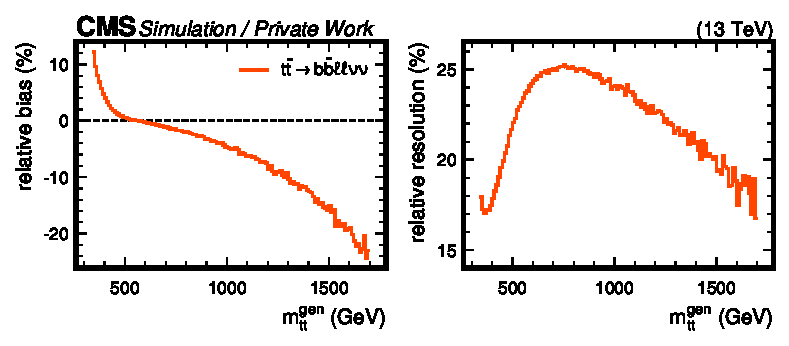
\includegraphics[width=0.99\linewidth]{figures/ah/mtt_resolution.pdf}
    \caption{Relative bias and resolution of the \ttbar reconstruction algorithm, defined in \cref{eq:ah:deltamtt}, as a function of truth-level \mtt and evaluated in MC simulation of dileptonic \ttbar.}
    \label{fig:ah:resolution}
\end{figure}

For $\ttbar \rightarrow \bbllnunu$ events passing all previous selection steps, the efficiency of the full reconstruction algorithm is ca. $90\%$, as evaluated in MC simulation. To asses the accuracy of the reconstruction relative to the truth-level top quarks, defined after parton showering, a per-event relative deviation is defined as 

\begin{equation}
\label{eq:ah:deltamtt}
    \Delta \mtt = \frac{\mtt^{\mathrm{reco}} - \mtt^{\mathrm{gen}}} {\mtt^{\mathrm{gen}}},
\end{equation}

\noindent where $\mtt^{\mathrm{reco}}$ and $\mtt^{\mathrm{gen}}$ stand for the reconstructed and truth-level \mtt, respectively. The mean and standard deviation of $\Delta \mtt$ are then the relative bias and resolution of the reconstruction algorithm. They are evaluated in simulation of dileptonic \ttbar and shown in \cref{fig:ah:resolution} as a function of truth-level \mtt. The method shows a bias towards high \mtt for events with $\mtt^{\mathrm{gen}} \lesssim \SI{600}{\GeV}$ and towards low \mtt for $\mtt^{\mathrm{gen}} \gtrsim \SI{600}{\GeV}$, with resolutions in the range of $17-25\%$. It should be noted here that this bias relative to the truth level is by itself not problematic for this analysis, since it is expected to be the same in both simulation and data and no unfolding of the reconstructed distributions to the truth level is attempted here.

\subsection{Sensitive observables}

To extract the A/H and \etat signals from the background, three sensitive observables are considered. The first is simply the invariant \ttbar mass \mtt, defined with the reconstruction procedure as explained in the last section. As shown in \cref{fig:theory:ahxs}, an A/H signal is expected to result in a peak-dip structure in \mtt around the SM background, where the zero crossing between peak and dip should be in the vicinity of the A/H mass, and the magnitude as well as ratio of the peak and the dip depends non-linearly on the coupling modifier. The \etat signal, on the other hand, is expected to peak slightly below the \ttbar production threshold at $\mtt \simeq 2 \mt - \SI{2}{GeV}$. In practice, due to the limited detector resolution, the exact position of this peak will not be observable, and the signal will result in a generic enhancement of the yield for very low values of \mtt.

In addition, the two spin correlation observables \chel and \chan, as defined in \cref{eq:theory:cheldef} and \cref{eq:theory:chan}, are used to gain further sensitivity. Both variables are again defined using the \ttbar system reconstruction as described in the previous section. As discussed in \cref{sec:theory:spindensity}, they are ideal for separating spin-singlet and spin-triplet states, respectively. Thus, A and \etat signals, producing singlet states, will have enhanced contributions at high values of \chel, while H signals, producing triplet states, will be enhanced at low values of \chan. This allows not only for better discrimination between signal and background, but also to distinguish whether a possible observed signal is scalar or pseudoscalar in nature. 

\begin{figure}[t]
    \centering
    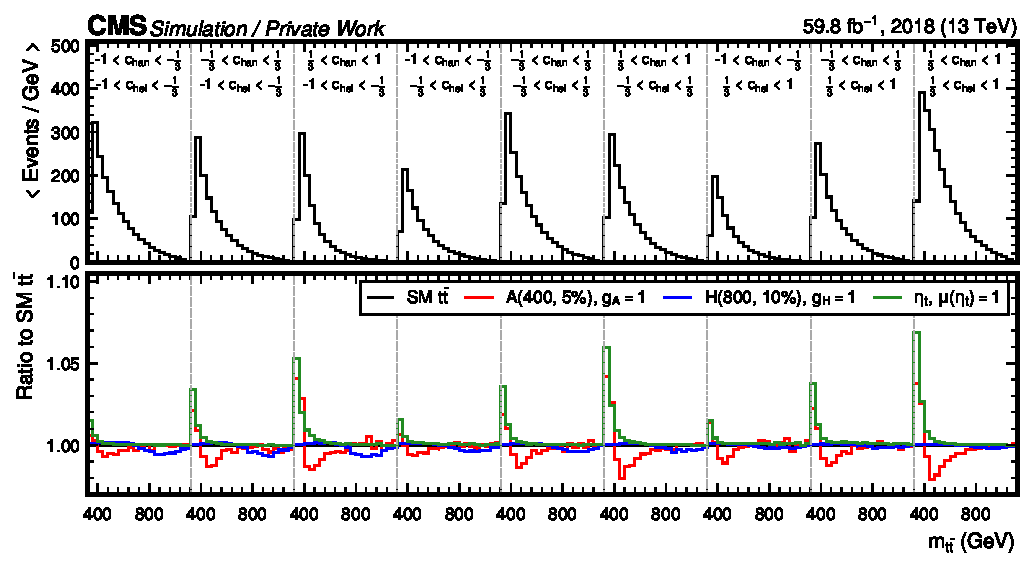
\includegraphics[width=0.99\linewidth]{figures/ah/mttchelchan.pdf}
    \caption{3D template for the three variables \mttchelchan for SM \ttbar (top) as well as three different example signals (bottom, shown as the ratio to SM \ttbar), corrsponding to the luminosity taken in 2018 only.}
    \label{fig:ah:mttchelchan}
\end{figure}


To combine all three variables, three-dimensional templates are created with $20 \times 3 \times 3$ bins in the three observables \mtt, \chel and \chan. For \mtt, an irregular binning is chosen to account for the decrease in production cross section at high values. An example can be seen in \cref{fig:ah:mttchelchan} for SM \ttbar and three different signals (A, H and \etat).

\section{Higher-order corrections in \ttbartitle}
\label{sec:ah:ttbarweights}

In this analysis, the SM \ttbar background is irreducible - after all, it leads to the exact same final state as the signal. As a result, it is crucial to model it as precisely as possible: a mis-modeling of the \ttbar kinematic distribution, especially in \mtt, might otherwise be confused for a signal and lead to bias.

The MC simulation used for the SM \ttbar background is performed a NLO in QCD using the \powhegvtwo subprocess \hvq, as studied also in \cref{ch:bb4l}. On top of this, two different sets of corrections are applied to include missing higher orders, namely NNLO QCD and NLO electroweak (EW) corrections. Both of these are estimated by comparing the MC simulation, which are matched to a parton shower, to fixed-order predictions. The simulation is then reweighted using scale factors binned two-dimensionally in \mtt and $\cost_t$, where the latter is the cosine of the scattering angle of the top quark to the beam axis in the \ttbar ZMF. In the SM, this variable is strongly correlated with the observables \chel and \chan, and is thus used in their place since spin correlation observables cannot be defined in calculations at stable top level.

\subsection{NNLO QCD corrections}

The NNLO QCD predictions are obtained with the program MATRIX~\cite{Grazzini:2017mhc}. They are computed at the level of stable top quarks with a dynamic scale choice of $\sqrt{\smash[b]{\mt^2+p_{T,t}^2}}$, where $p_{T,t}$ is the top quark transverse momentum. \cref{fig:ah:ewqcdcorrs} shows the resulting effect on the 3D \mttchelchan distribution at the detector level as the black line. They are on the order of $1-2\%$.

\begin{figure}[t]
    \centering
    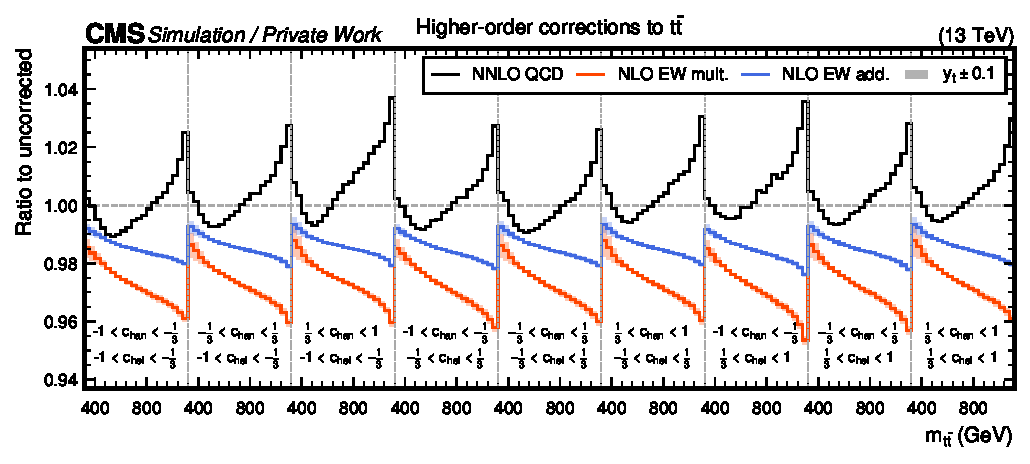
\includegraphics[width=0.99\linewidth]{figures/ah/ewqcdcorrs.pdf}
    \caption{Effect of NNLO QCD and NLO EW corrections on the 3D \mttchelchan distribution after reconstruction in the form of ratios to the uncorrected distributions. The NNLO QCD corrections are shown as the solid black line, while the NLO EW corrections are shown in orange for the multiplicative scheme and in blue for the additive scheme. The effect of varying \yt by $\pm 0.1$ in the NLO EW corrections is shown as the shaded bands.}
    \label{fig:ah:ewqcdcorrs}
\end{figure}

\subsection{NLO EW corrections}
\label{sec:ah:ewcorr}

\begin{figure}[t]
    \centering
    \begin{tikzpicture}
      \begin{feynman}
        \vertex (i1) {\(g\)};
        \vertex [below=2.0 cm of i1] (i2) {\(g\)};
        \vertex [right=1.5 cm of i1] (a);
        \vertex [right=1.5 cm of i2] (b);
        \vertex [right=1.5 cm of a] (c);
        \vertex [right=1.5 cm of b] (d);
        \vertex [right=1.5 cm of c] (f1) {\(t\)};
        \vertex [right=1.5 cm of d] (f2) {\(\bar{t}\)};
        \diagram* {
          (i1) -- [gluon] (a),
          (i2) -- [gluon] (b),
          (c) -- [scalar, edge label=\(h\)] (d),
          (f1) -- [anti fermion] (c) -- [anti fermion] (a) -- [anti fermion, edge label=\(t\)] (b) -- [anti fermion] (d) -- [anti fermion] (f2)
        };
      \end{feynman}
    \end{tikzpicture}
    \caption{\textbf{EW correction involving a SM Higgs boson.} An example Feynman diagram for NLO EW corrections to \ttbar production involving the exchange of a virtual SM Higgs boson $h$.}
    \label{fig:ah:ewcorr_feynman}
\end{figure}

The NLO corrections in the electroweak coupling \alphaew are computed with the HATHOR code~\cite{Aliev:2010zk, Kuhn:2005it, Kuhn:2006vh, Kuhn:2013zoa} using the same nominal scale choices. Of particular interest here is a class of diagrams which contain an exchange of a virtual SM Higgs boson, an example of which is seen in \cref{fig:ah:ewcorr_feynman}. The matrix element for this diagram is proportional to the square of the SM Higgs-top Yukawa coupling \yt, giving a $\yt^2$-dependent correction to \ttbar distributions from the interference with LO diagrams. This correction is sizeable mostly for low \mtt values, and is important for this analysis because the SM Higgs exchange might change the \ttbar spin state and thus \chel and \chan. To accurately account for this, the correction is derived separately for the different initial states ($gg$, $q\bar{q}$ and $gq$) of \ttbar production.

The results obtained with HATHOR are accurate only to LO in \alphas, i.e. \order{\alphas^2}, and as of the time of writing no full calculation including both NLO QCD and EW effects exists. Thus, there is an ambiguity on how the NLO-accurate (in QCD) MC simulation and the NNLO-accurate corrections presented in the previous section should be combined with the EW corrections.

Formally, the differential cross section as predicted by Powheg can be decomposed as

\begin{equation}
    d \sigma_{\powheg} = \alphas^2 d \sigma_{\mathrm{LO}} + \alphas^3 d \sigma_{\mathrm{NLO}}
\end{equation}

\noindent where additional terms beyond $\order{\alphas^3}$ due to additional radiation in Powheg and Pythia are not written for simplicity. On the other hand, HATHOR predicts

\begin{equation}
    d \sigma_{\mathrm{HATHOR}} = \alphas^2 d \sigma_{\mathrm{LO}} + \alphas^2 \alphaew d \sigma_{\mathrm{EW}}.
\end{equation}

One possible way to combine the calculations is the additive scheme, given by


\begin{equation}
\begin{split}
\label{eq:ah:ewadd}
    d \sigma_{\mathrm{add.}} &= d \sigma_{\powheg} + d \sigma_{\mathrm{HATHOR}} - \alphas^2 d \sigma_{\mathrm{LO}} \\
    &= \alphas^2 d \sigma_{\mathrm{LO}} + \alphas^3 d \sigma_{\mathrm{NLO}} + \alphas^2 \alphaew d \sigma_{\mathrm{EW}}
\end{split}
\end{equation}

\noindent which is formally accurate to $\order{\alphas^3}$ and $\order{\alphas^2 \alphaew}$. This approach does not include any cross terms of order $\order{\alphas^3 \alphaew}$, which are not fully calculated by either Powheg or HATHOR. However, it is reasonable to assume \todo{ref} that these cross terms factorize approximately, leading to the alternative multiplicative scheme

\begin{equation}
\begin{split}
\label{eq:ah:ewmult}
    d \sigma_{\mathrm{mult.}} &= d \sigma_{\powheg} \times \frac{d \sigma_{\mathrm{HATHOR}}} {\alphas^2 d \sigma_{\mathrm{LO}}} \\
    &= \alphas^2 d \sigma_{\mathrm{LO}} + \alphas^3 d \sigma_{\mathrm{NLO}} + \alphas^2 \alphaew d \sigma_{\mathrm{EW}} + \alphas^3 \alphaew \frac {d \sigma_{\mathrm{NLO}} \, d \sigma_{\mathrm{EW}}}{d \sigma_{\mathrm{LO}}}
\end{split}
\end{equation}

The difference between the two schemes is in the last term of order $\order{\alphas^3\alphaew}$, which is an approximation to the QCD-EW cross terms. In this work, the multiplicative approach is used for all nominal results, while the difference to the additive approach is included as a systematic uncertainty. In both cases, the needed term $d \sigma_{\mathrm{LO}}$ is computed with MadGraph 5.

The effect of both approaches on the 3D \mttchelchan distribution at the detector level after parton showering can be seen in \cref{fig:ah:ewqcdcorrs} for different values of \yt. The multiplicative scheme leads to a larger correction of roughly $2-4\%$, while the additive scheme only gives $1-2\%$. Notably, the effect of varying \yt modifies not only the \mtt distribution close to the \ttbar threshold, but also the distribution of \chel. As a result, such a variation in data could potentially be confused for a pseudoscalar signal. It is thus important to include it as a systematic uncertainty, as described in \cref{sec:ah:systs}.


\section{Matrix element reweighting for \AH signals}
\label{sec:ah:mereweighting}

In order to probe the full phase space of the generic \AH model as described in \cref{sec:ah:intro}, predictions at different \AH masses and widths with a sufficiently small spacing are required so that interpolation between the points is possible. However, generating a separate MC sample for each mass and width point is computationally very expensive.

\subsection{Principle of the method}

As an alternative, it is possible to re-use existing samples for different mass and width points via matrix-element reweighting. This method works by noting that a given MC sample can be seen as a random sample, drawn from a PDF of the form

\begin{equation}
\label{eq:ah:merewprob}
    \mathcal{P}(x_i^{\mathrm{ME}}, x_j^{\mathrm{reco}}) = \mathcal{P}^{\mathrm{ME}} (x_i^{\mathrm{ME}}) \cdot \mathcal{P}^{\mathrm{rem}} (x_j^{\mathrm{reco}} | x_i^{\mathrm{ME}})
\end{equation}

Here, $x_i^{\mathrm{ME}}$ are all variables defining the event at the matrix element (ME) level, i.e. at the level of the hard interaction, and $x_j^{\mathrm{reco}}$ are all variables after detector simulation and object reconstruction. For the case of the \AH signals, which are generated at LO in QCD, $x_i^{\mathrm{ME}}$ is given fully by the four-momenta and helicities of the final-state particles (leptons, neutrinos and b quarks) in the hard process. The $x_j^{\mathrm{reco}}$ consist of all possible reconstruction-level variables that are relevant to the analysis, such as e.g. jet and lepton four-momenta, lepton identification criteria or \ptmissvec. 

$\mathcal{P}^{\mathrm{ME}} (x_i^{\mathrm{ME}})$ refers to the probability density of the ME-level variables as predicted by the ME generator, which will be proportional to the absolute square of the matrix element. This function will depend on the chosen scenario of the \AH model, i.e. $m_{\AH}$ and $\Gamma_{\AH}$. Meanwhile, the conditional probability density $\mathcal{P}^{\mathrm{rem}} (x_j^{\mathrm{reco}} | x_i^{\mathrm{ME}})$ encodes the effects of all other components of the simulation chain, such as the parton shower, hadronization, detector simulation and reconstruction. It gives the probability to observe reconstruction-level variables $x_j^{\mathrm{reco}}$ for an event with ME-level variables $x_i^{\mathrm{ME}}$.

The principal assumption of the method is now that $\mathcal{P}^{\mathrm{rem}}$, and thus the whole simulation chain except for the matrix element, is independent of the underlying \AH signal scenario ($m_{\AH}$ and $\Gamma_{\AH}$). This assumption is certainly true for the detector simulation and reconstruction, while care must be taken for the parton shower, which in general needs to be matched to the matrix element and can this way have a residual dependence. The validity of the assumption will be discussed in more detail below.

If the assumption is fulfilled, a given \AH MC sample generated with parameters $m_{\AH}^0$ and $\Gamma_{\AH}^0$ can now be reweighted to a different \AH scenario with parameters $\hat{m}_{\AH}$ and $\hat{\Gamma}_{\AH}$ by applying to each event $i$ a weight 

\begin{equation}
\label{eq:ah:merewweight}
    w_i = \frac{ \mathcal{P}^{\mathrm{ME}} (x_i^{\mathrm{ME}} | \hat{m}_{\AH} , \hat{\Gamma}_{\AH} ) } { \mathcal{P}^{\mathrm{ME}} (x_i^{\mathrm{ME}} | m_{\AH}^0 , \Gamma_{\AH}^0 ) }
\end{equation}

The quantities in the denominator and nominator are the ME-level probability densities for each event, evaluated at the original and target \AH parameters, respectively. When this weight is inserted into \cref{eq:ah:merewprob}, the original probability cancels, giving the correct probability density for the target scenario $\hat{m}_{\AH}$ and $\hat{\Gamma}_{\AH}$.

In practice, this method will only work if the MC sample used for the reweighting has sufficient phase space overlap with the target \AH scenario, i.e. if the two probabilities in \cref{eq:ah:merewweight} are not too different from each other for the majority of the events. Otherwise, the weights will become very small in some regions of the phase space and very large in others, resulting in poor statistics for the reweighted sample.

The method was implemented by directly evaluating the squared matrix elements for the different \AH hypotheses, using the standalone reweighting interface provided by MadGraph 5 and the same UFO model as for the signal generation. 

\subsection{Combination of multiple origin samples}

For the purpose of this analysis, a set of signal samples for different \AH scenarios (as given in \cref{sec:ah:datasets}) was already available at the time of starting these studies. These samples were used as origin samples for the reweighting. In order to maximize the statistics achieved after reweighting for each target \AH scenario, and mitigate problems from poor phase space overlap, a subset of the available samples were combined after reweighting for each target scenario.

This procedure works as follows: First, a set of several origin samples $j$ with different parameters $m_{\AH}$ and $\Gamma_{\AH}$ are all reweighted separately to the same target parameters $\hat{m}_{\AH}$ and $\hat{\Gamma}_{\AH}$ with per-event weights $w_{i,j}$ as given in \cref{eq:ah:merewweight}. Then, the different samples are again weighted with a per-sample weight $v_j$, given by

\begin{equation}
    v_j = {\langle w_{i,j} \rangle}^{-1} =  \frac{ \sum_i w_{i,j} }{ \sum_i w_{i,j}^2 }
\end{equation}

\noindent where the sums run over all events $i$ in the considered sample $j$. This expression is the inverse of the average ME weight for sample $j$. It is chosen such that samples with large phase space overlap with the target \AH scenario - and thus small ME weights $w_{i,j}$ - are assigned a large weight $v_j$ in the combination of samples. Similarly, samples with poor phase space overlap, and thus large average ME weights, get assigned small weights and contribute less strongly to the combined sample. \todo{check whether this actually minimizes anything.}

In practice, all available masses and parities (A and H) are combined for each target \AH mass. Resonance and interference contributions are treated separately from each other. Furthermore, it was found that, for the resonance contribution only, it is necessary to split the combination of different \AH widths into two halves: those with $\wAH/\mAH$ less or greater than 10\%. This is due to a dependency of the Pythia shower on the \AH width in the matrix element, which is not taken into account in the reweighting. For $\wAH/\mAH < 10\%$ (narrow resonance), Pythia treats the intermediate \AH particle as a unstable resonance, and attempts to preserve its virtuality as predicted by the matrix element, while no such attempt is made for $\wAH/\mAH \geq 10\%$ (broad resonance) \todo{check}. This leads to slight differences in distributions affected by the parton showering. The choice of 10\% for the transition between the two modes is an arbitrary parameter, and thus not necessarily physical. Nonetheless, it was decided in this analysis to not mix the two width ranges in the reweighting in order to obtain full closure with a stand-alone generation.

\subsection{Validation}

The combined reweighting is validated for three masses of $\mAH = 400$, 600 and 800 GeV as well as widths of 2.5 and 10\%. For each of these points, the reweighting is performed as stated above, but leaving out \AH scenarios with the same mass from the combination of origin samples since otherwise the weights would be trivially one. The reweighted \mtt distributions at generator level are then compared to the stand-alone samples at the same \mAH and \wAH.

The resulting comparisons and residuals can be seen in \cref{fig:ah:merew_validation_A,fig:ah:merew_validation_H} for A and H, respectively, separated into the resonance and interference contributions. It can be seen that the closure between reweighting and standalone generation is excellent within the statistical uncertainties.

\begin{figure}[h]
    \centering
    \begin{subfigure}[b]{0.49\textwidth}
        \centering
        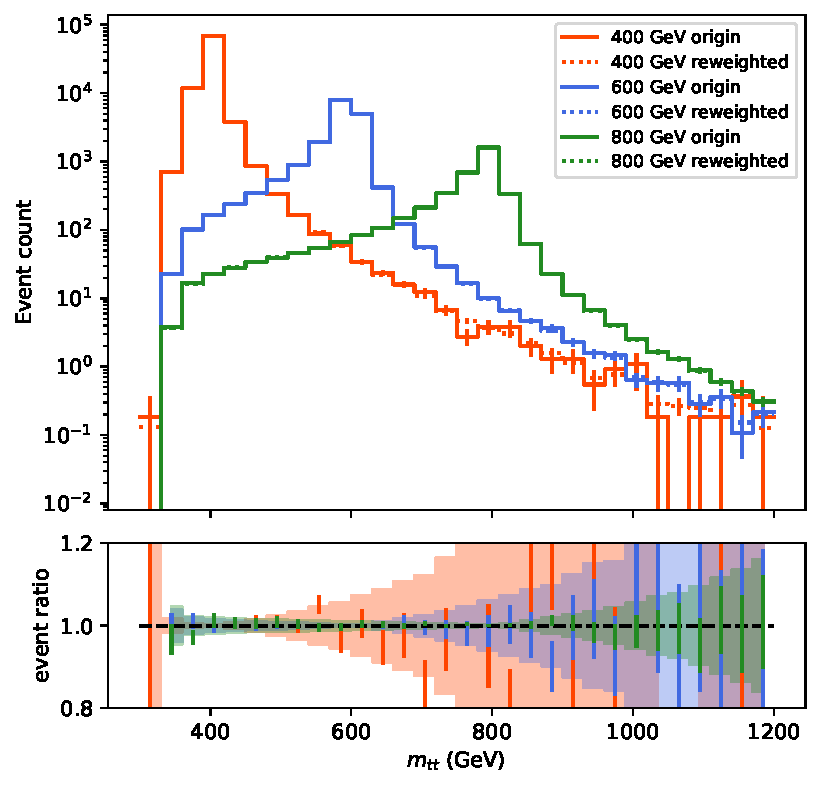
\includegraphics[width=\textwidth]{figures/ah/me_reweighting/A_res_2p5_mtt_log_pos.pdf}
        \caption{A, $\wA/\mA = 2.5\%$, resonance}
    \end{subfigure}
    \hfill
    \begin{subfigure}[b]{0.49\textwidth}
        \centering
        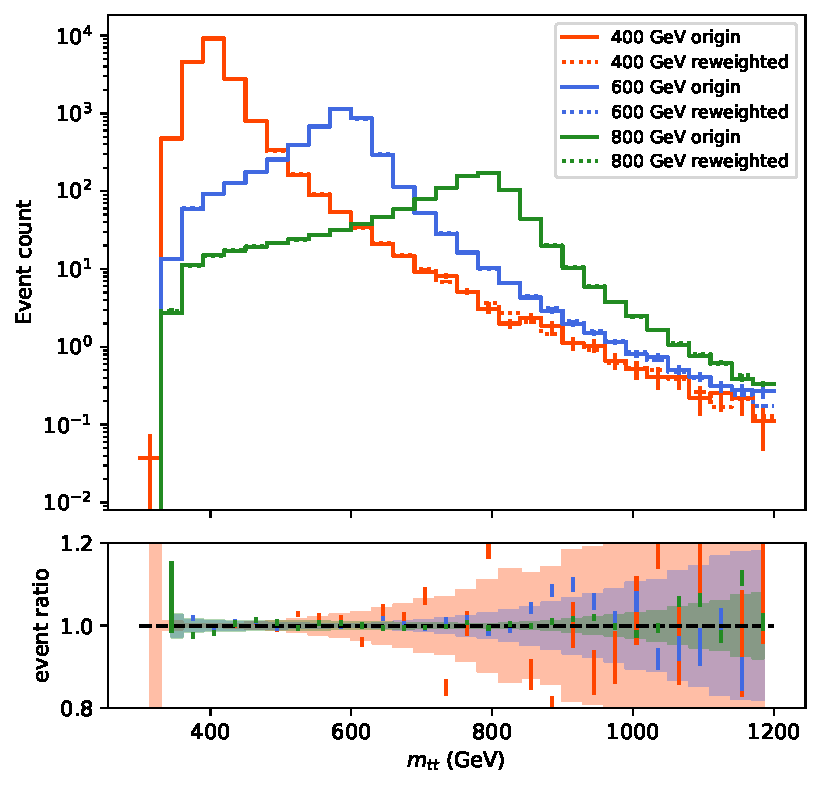
\includegraphics[width=\textwidth]{figures/ah/me_reweighting/A_res_10p0_mtt_log_pos.pdf}
        \caption{A, $\wA/\mA = 10\%$, resonance}
    \end{subfigure}
    \begin{subfigure}[b]{0.49\textwidth}
        \centering
        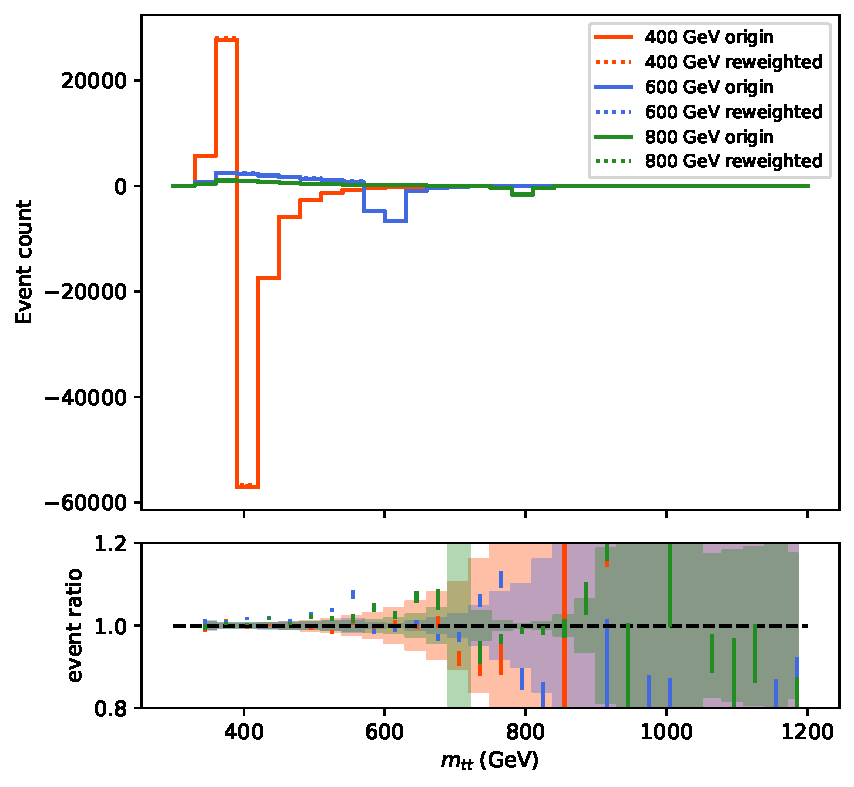
\includegraphics[width=\textwidth]{figures/ah/me_reweighting/A_int_2p5_mtt_diff.pdf}
        \caption{A, $\wA/\mA = 2.5\%$, interference}
    \end{subfigure}
    \hfill
    \begin{subfigure}[b]{0.49\textwidth}
        \centering
        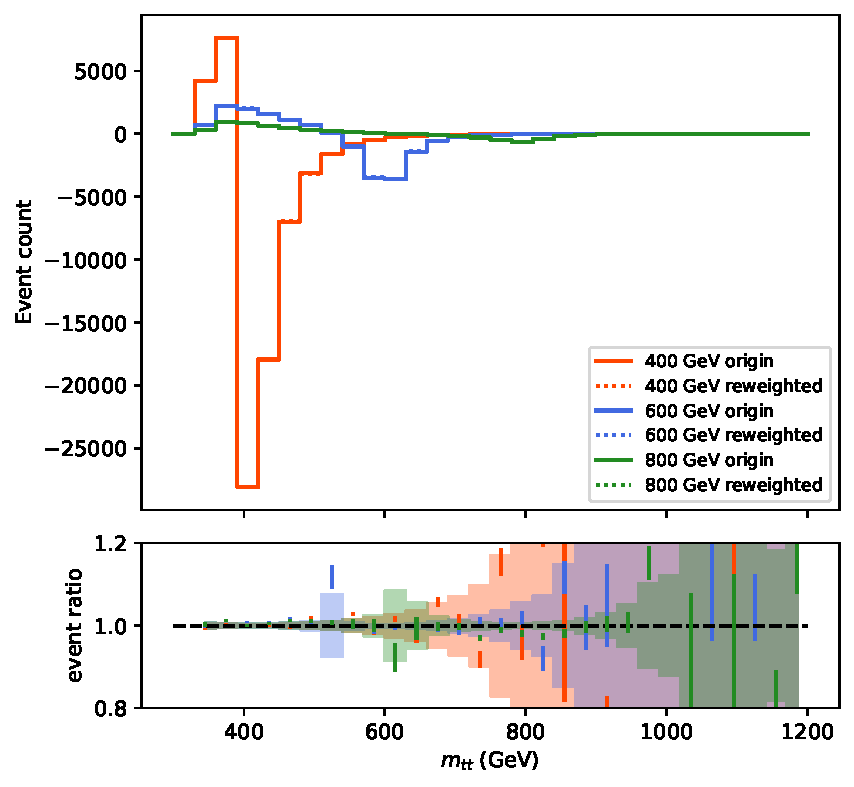
\includegraphics[width=\textwidth]{figures/ah/me_reweighting/A_int_10p0_mtt_diff.pdf}
        \caption{A, $\wA/\mA = 10\%$, interference}
    \end{subfigure}
    \caption{\textbf{Validation of the ME reweighting for A.} Comparison of standalone generated (solid) and reweighted (dashed) \mtt distributions for different values of \mA. The lower panel shows the ratio of reweighted and standalone distributions. The error bars and colored areads give the statistical uncertainty of the reweighted and standalone sample, respectively.}
    \label{fig:ah:merew_validation_A}
\end{figure}

\begin{figure}[h]
    \centering
    \begin{subfigure}[b]{0.49\textwidth}
        \centering
        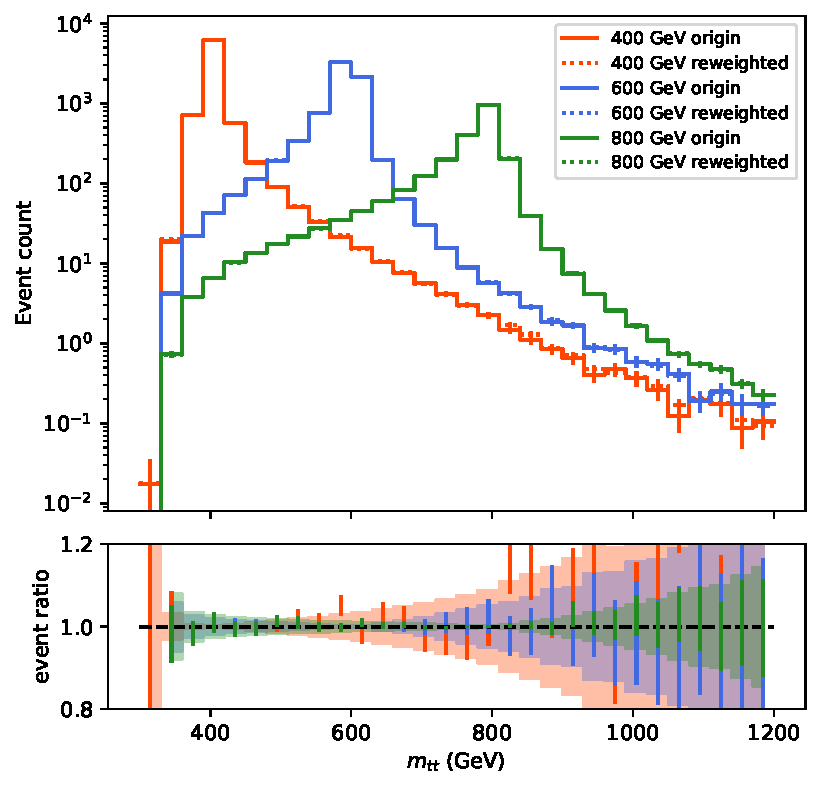
\includegraphics[width=\textwidth]{figures/ah/me_reweighting/H_res_2p5_mtt_log_pos.pdf}
        \caption{H, $\wH/\mH = 2.5\%$, resonance}
    \end{subfigure}
    \hfill
    \begin{subfigure}[b]{0.49\textwidth}
        \centering
        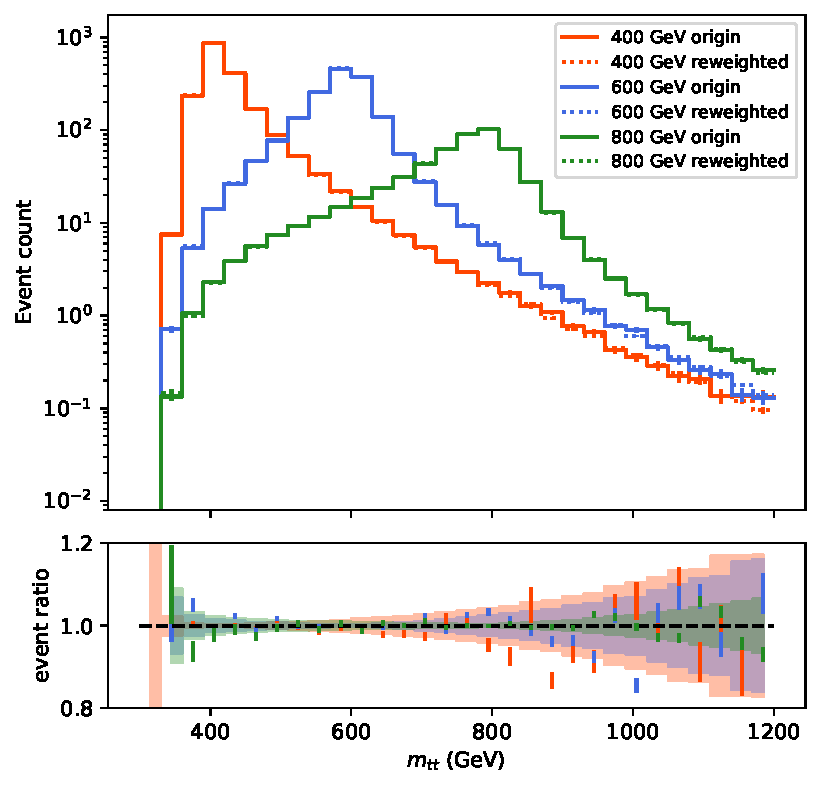
\includegraphics[width=\textwidth]{figures/ah/me_reweighting/H_res_10p0_mtt_log_pos.pdf}
        \caption{H, $\wH/\mH = 10\%$, resonance}
    \end{subfigure}
    \begin{subfigure}[b]{0.49\textwidth}
        \centering
        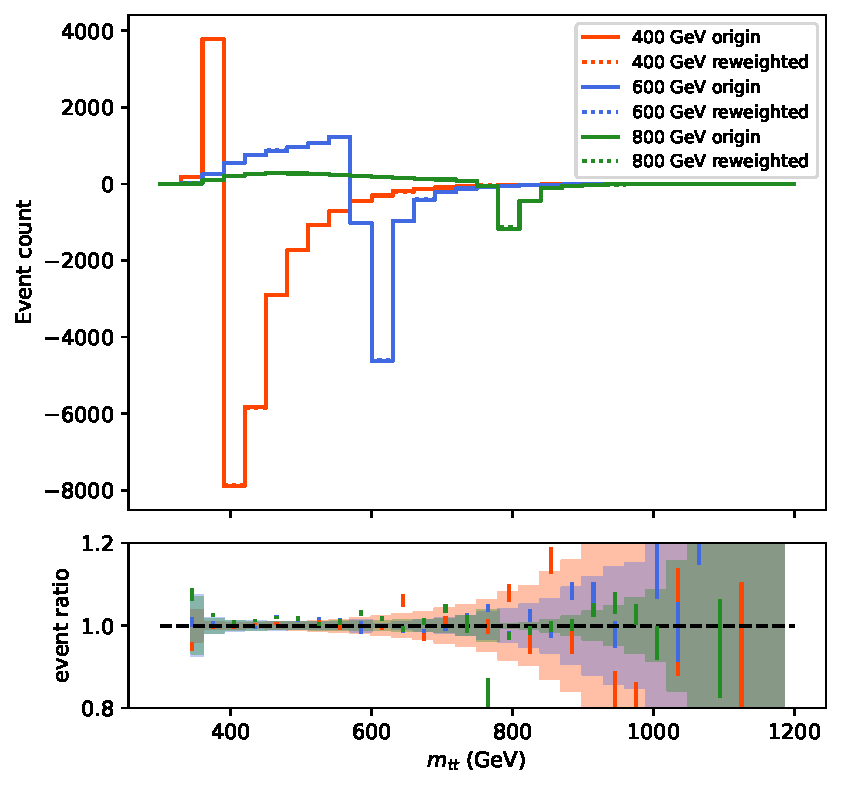
\includegraphics[width=\textwidth]{figures/ah/me_reweighting/H_int_2p5_mtt_diff.pdf}
        \caption{H, $\wH/\mH = 2.5\%$, interference}
    \end{subfigure}
    \hfill
    \begin{subfigure}[b]{0.49\textwidth}
        \centering
        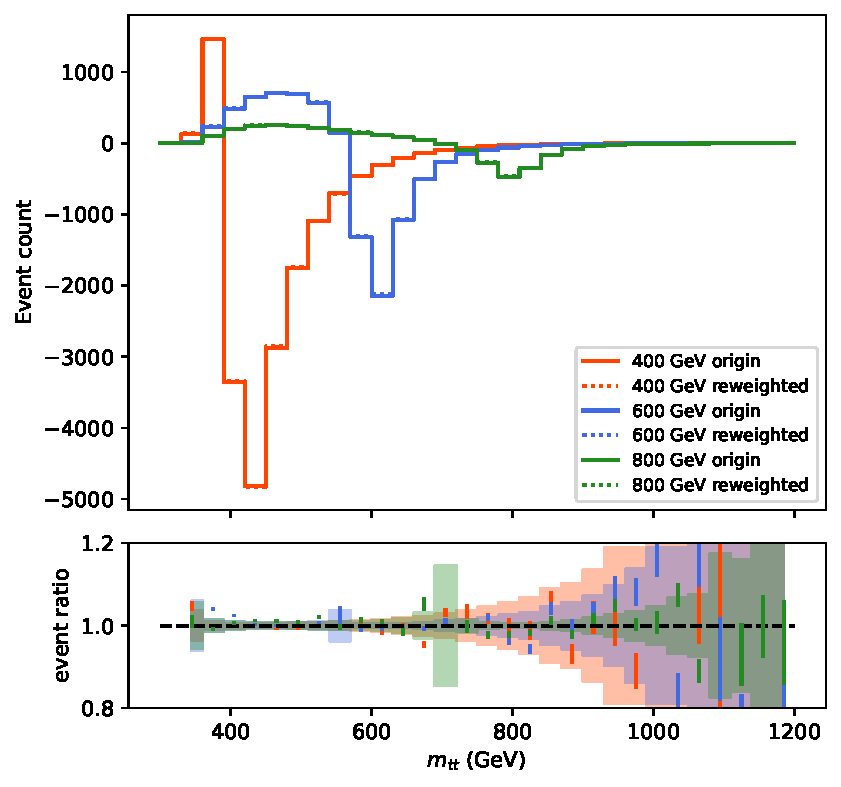
\includegraphics[width=\textwidth]{figures/ah/me_reweighting/H_int_10p0_mtt_diff.pdf}
        \caption{H, $\wH/\mH = 10\%$, interference}
    \end{subfigure}
    \caption{\textbf{Validation of the ME reweighting for H.} Comparison of standalone generated and reweighted \mtt distributions for different values of \mH, similar to \cref{fig:ah:merew_validation_A}.}
    \label{fig:ah:merew_validation_H}
\end{figure}

\section{Systematic uncertainties}
\label{sec:ah:systs}

Similar to \cref{sec:ttxs:systematics}, systematic uncertainties affect the distributions of both SM background and signal processes. They are listed in this section, split into theory (\cref{sec:ah:theorysysts}) and experimental uncertainties (\cref{sec:ah:expsysts}).

\subsection{Theory uncertainties}
\label{sec:ah:theorysysts}

\paragraph{Scale uncertainties.}
Uncertainties due to missing higher orders in the matrix element as well as the parton shower are included separately for the SM \ttbar, tW, \Zgamma+jets backgrounds as well as all considered signals by varying the associated scales by a factor 2 up and down independently, same as in \cref{sec:ttxs:systematics}. For A and H, the uncertainties are considered uncorrelated between the resonance and interference components, which is found to be conservative. For \etat, the renormalization scale uncertainty is not included since the considered model does not encode any dependence on either $\mu_R$ or \alphas.

\paragraph{PDF uncertainties.}
For the SM \ttbar background, the uncertainty due to the PDF is again included based on the 100 provided eigenvalues of the used NNPDF 3.1 PDF set. However, it is not considered sufficient to simply take the envelope of these variations since this would distort possible shape variations. Instead, a principal component analysis (PCA) is performed on the final 3D templates obtained from the different eigenvalues, thus finding those linear combinations that have a noticable shape effect. It is found that only the first eigenvector (corresponding to the largest eigenvalue) is non-negligible, and variation is considered as the PDF uncertainty. Independently of this, another uncertainty based on the value of \alphas in the PDF is considered similarly to \cref{sec:ttxs:systematics}.

\paragraph{EW correction uncertainties.}
As described in \cref{sec:ah:ewcorr}, two independent uncertainties are attached to the NLO electroweak correction of SM {\ttbar}: First, the value of the SM top-Higgs Yukawa coupling is allowed to vary in the range $\yt = {1.00}^{+0.11}_{-0.11}$, with the range given by the uncertainty of the experimental measurement in \citere{CMS:HIG-17-031}. Second, the difference between the additive and multiplicative application scheme (\cref{eq:ah:ewadd,eq:ah:ewmult}) is considered as a seperate uncertainty, as recommended in \citere{Kuhn:2013zoa}, and symmetrized around the nominal.

\paragraph{Top quark mass uncertainty.}
The top quark mass uncertainty in SM \ttbar is estimated by varying it from its nominal value of $\mt = \SI{172.5}{\GeV}$ by $\pm \SI{3}{\GeV}$ in the \powheg simulation, and then scaling down the resulting relative deviation by a factor $1/3$, leading to a $\pm \SI{1}{\GeV}$ uncertainty. This is done since the variation, obtained from an independent MC sample, is otherwise plagued by large statistical uncertainties. Furthermore, the top mass is also varied in all considered signal samples directly by $\pm \SI{1}{\GeV}$ through an ME reweighting method similar to \cref{sec:ah:mereweighting}. The top mass uncertainties between background and signals are considered as fully correlated.

\paragraph{Further uncertainties in SM \ttbar.}
Additionally, separate SM \ttbar samples are used to evaluate uncertainties due to ME/PS matching (same as in \cref{sec:ttxs:systematics}), the underlying event tune~\cite{CMS:GEN-17-001}, and the color reconnection model in \pythia~\cite{CMS:GEN-17-002,Christiansen:2015yqa}. All of these effects are found to be small in the channels considered here.

\paragraph{Background cross section uncertainties.}
For the SM \ttbar background, instead of including an explicit cross section uncertainty, the shift in the predicted NNLO+NNLL \ttbar cross section due to the ME scales and the top quark mass is correlated with the respective uncertainties. For minor backgrounds, explicit uncertainties of 15\% for tW and t-channel single top, 30\% for diboson and \ttbar+X, and 5\% for the data-driven \Zgamma+jets normalization are considered.

\paragraph{Background statistical uncertainties.}
Again similar to \cref{sec:ttxs:systematics}, per-bin background statistical uncertainties for all simulated processes are included following \citere{Barlow:1993dm}.

\subsection{Experimental uncertainties}
\label{sec:ah:expsysts}

\paragraph{Lepton uncertainties.}

\paragraph{Jet and \ptmiss uncertainties.}

\paragraph{b tagging uncertainties.}

\paragraph{Trigger uncertainties.}

\paragraph{Luminosity uncertainty.}

\paragraph{Pileup uncertainty.}

\subsection{Uncertainty smoothing}

\section{Pre-fit distributions}
\label{sec:ah:prefit}

\begin{figure}[!p]
    \centering
    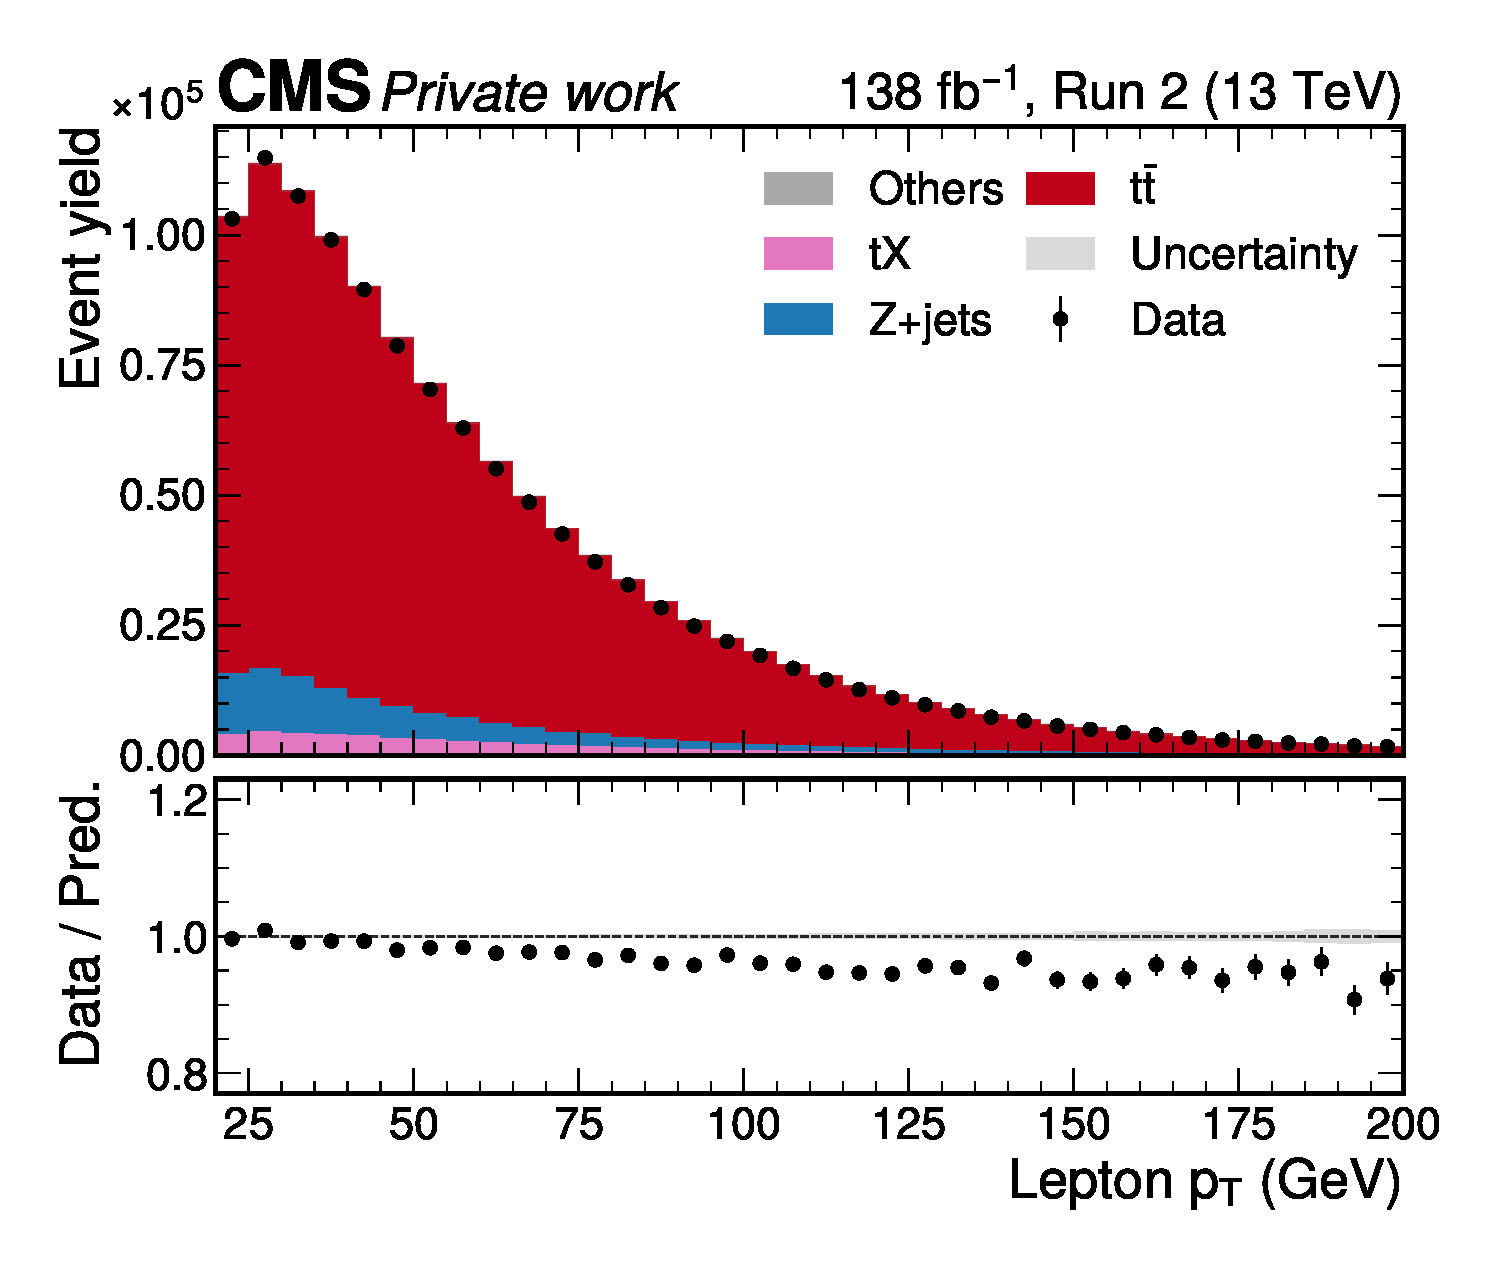
\includegraphics[width=0.49\textwidth]{figures/ah/controlplots/Req MET/sf/Leptonpt_Req MET_sf.pdf}
    \hfill
    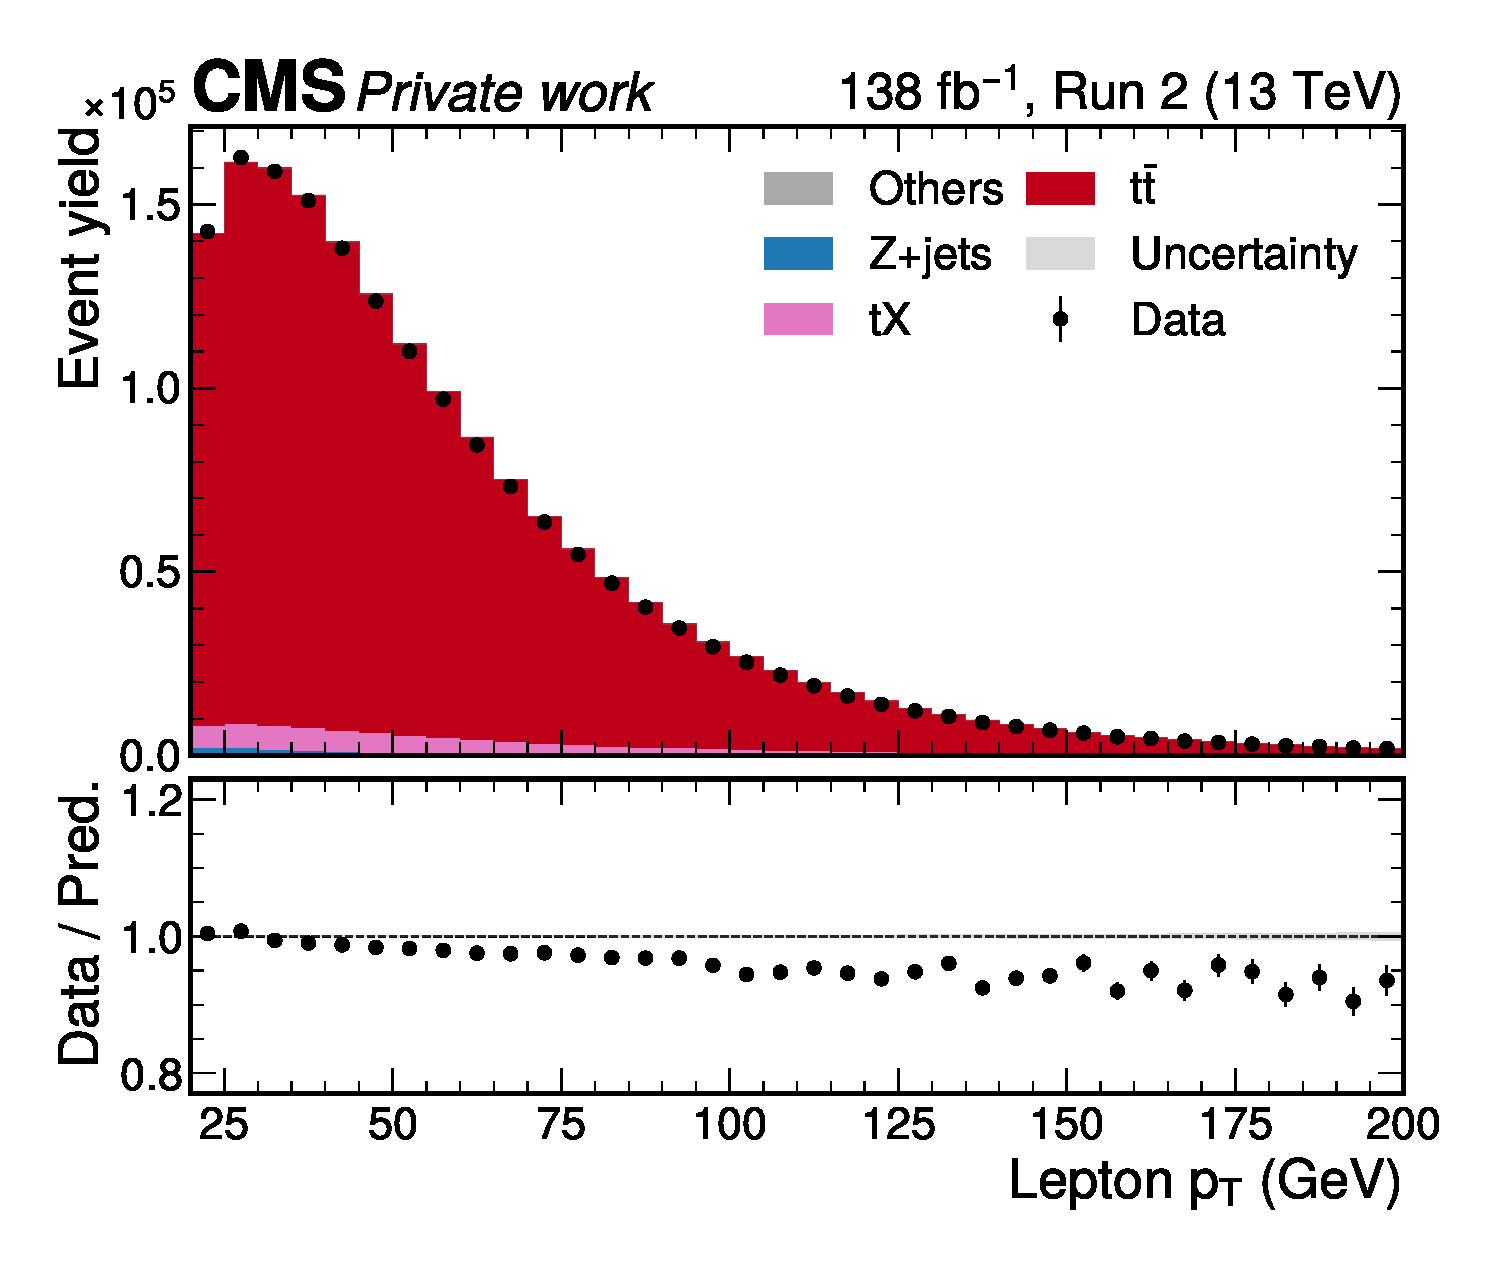
\includegraphics[width=0.49\textwidth]{figures/ah/controlplots/Req MET/em/Leptonpt_Req MET_em.pdf}
    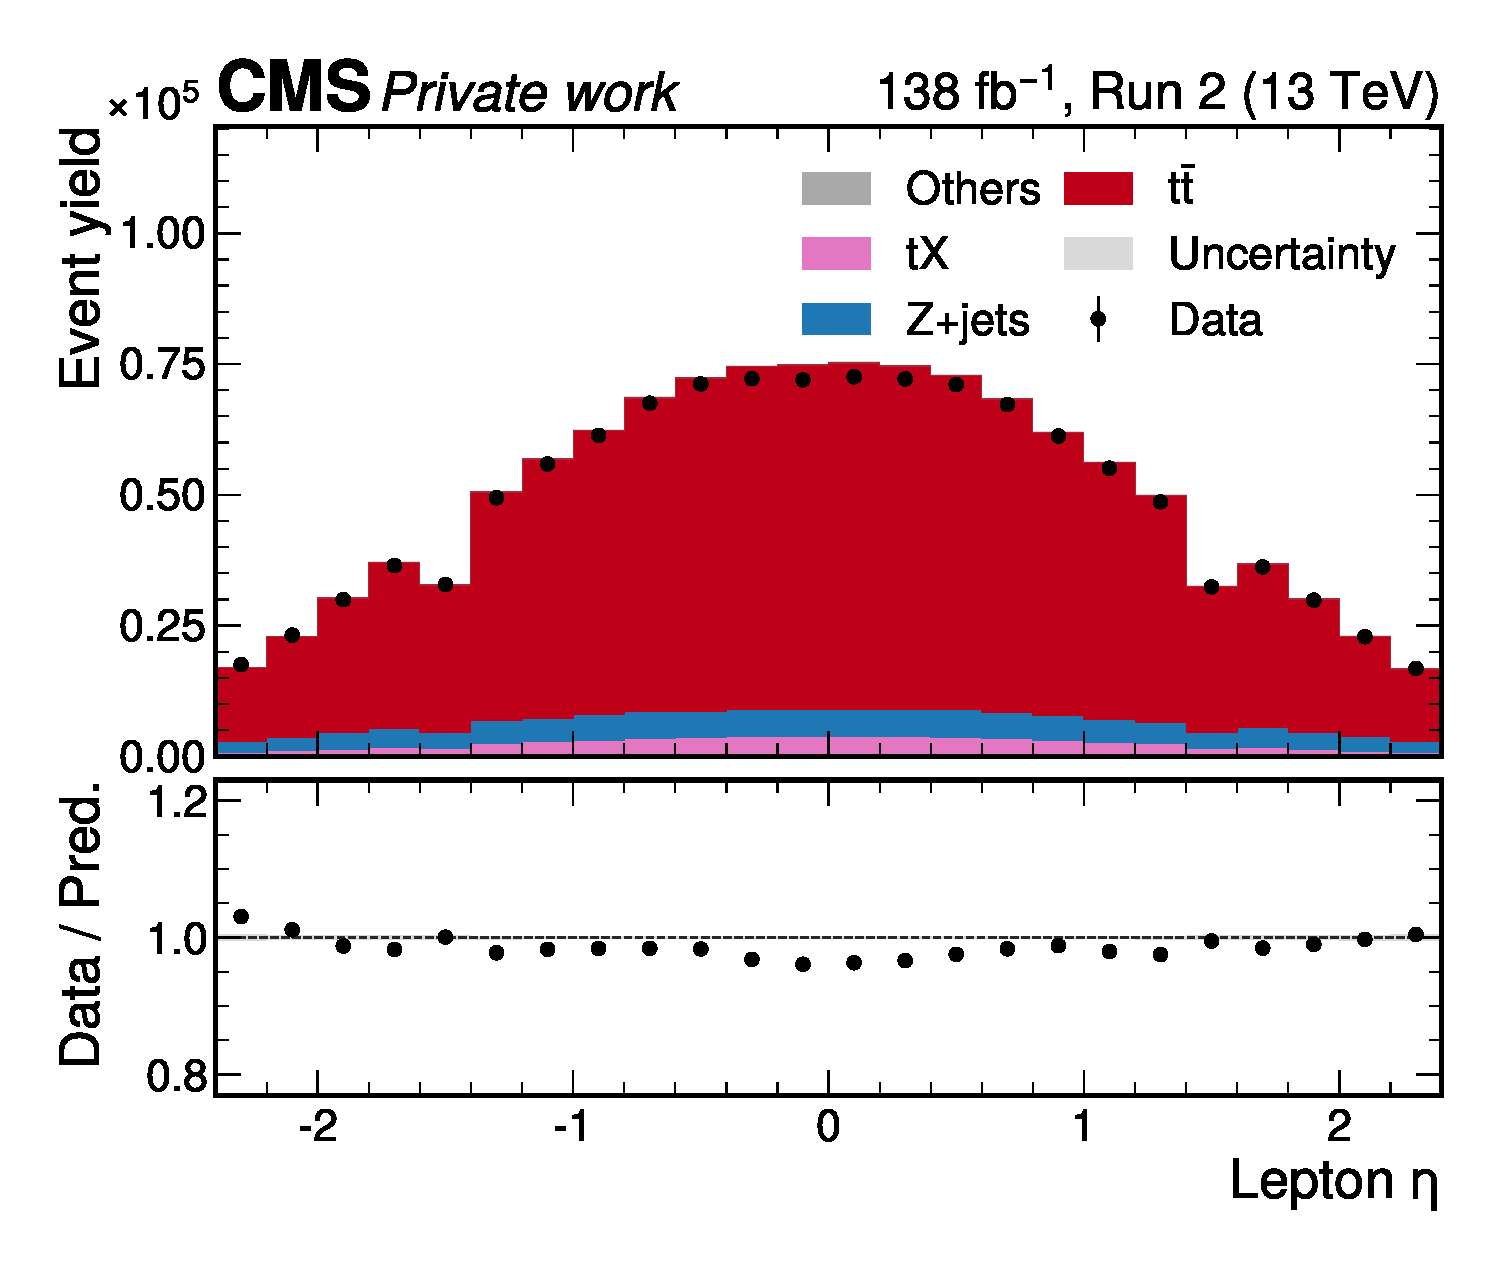
\includegraphics[width=0.49\textwidth]{figures/ah/controlplots/Req MET/sf/Leptoneta_Req MET_sf.pdf}
    \hfill
    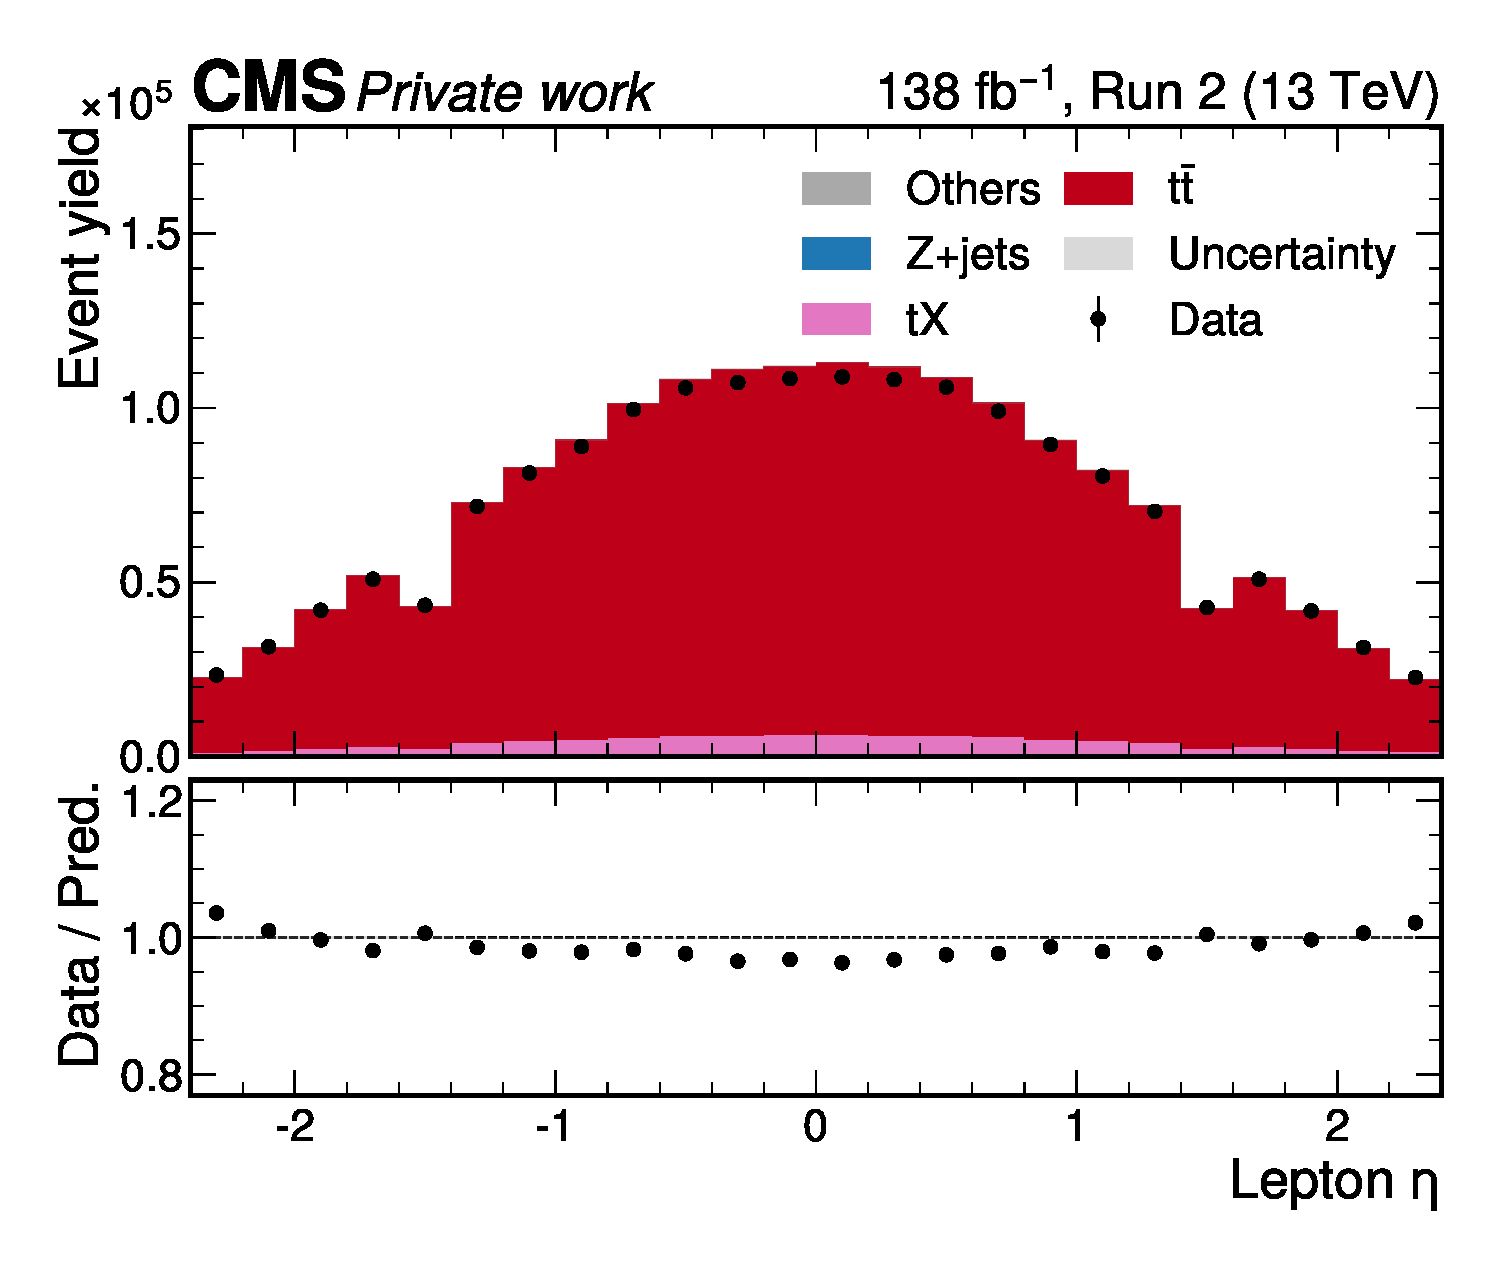
\includegraphics[width=0.49\textwidth]{figures/ah/controlplots/Req MET/em/Leptoneta_Req MET_em.pdf}
    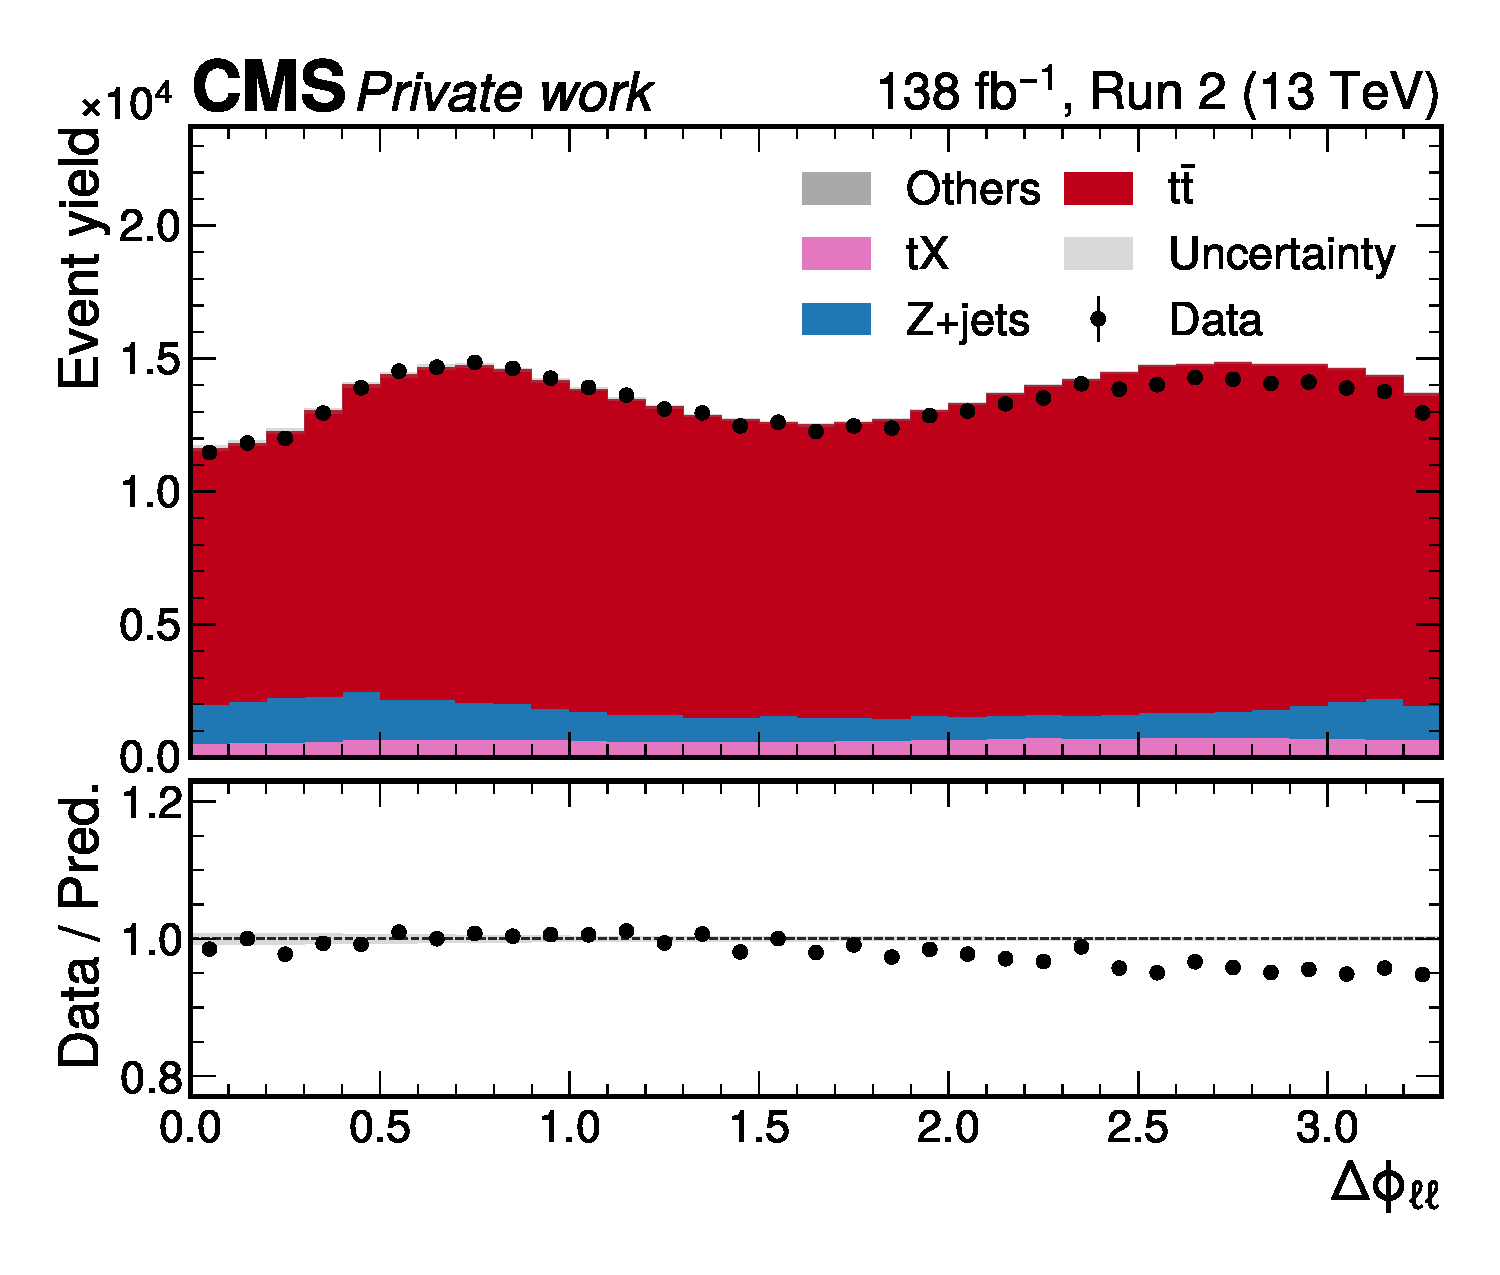
\includegraphics[width=0.49\textwidth]{figures/ah/controlplots/Req MET/sf/deltaphi_Req MET_sf.pdf}
    \hfill
    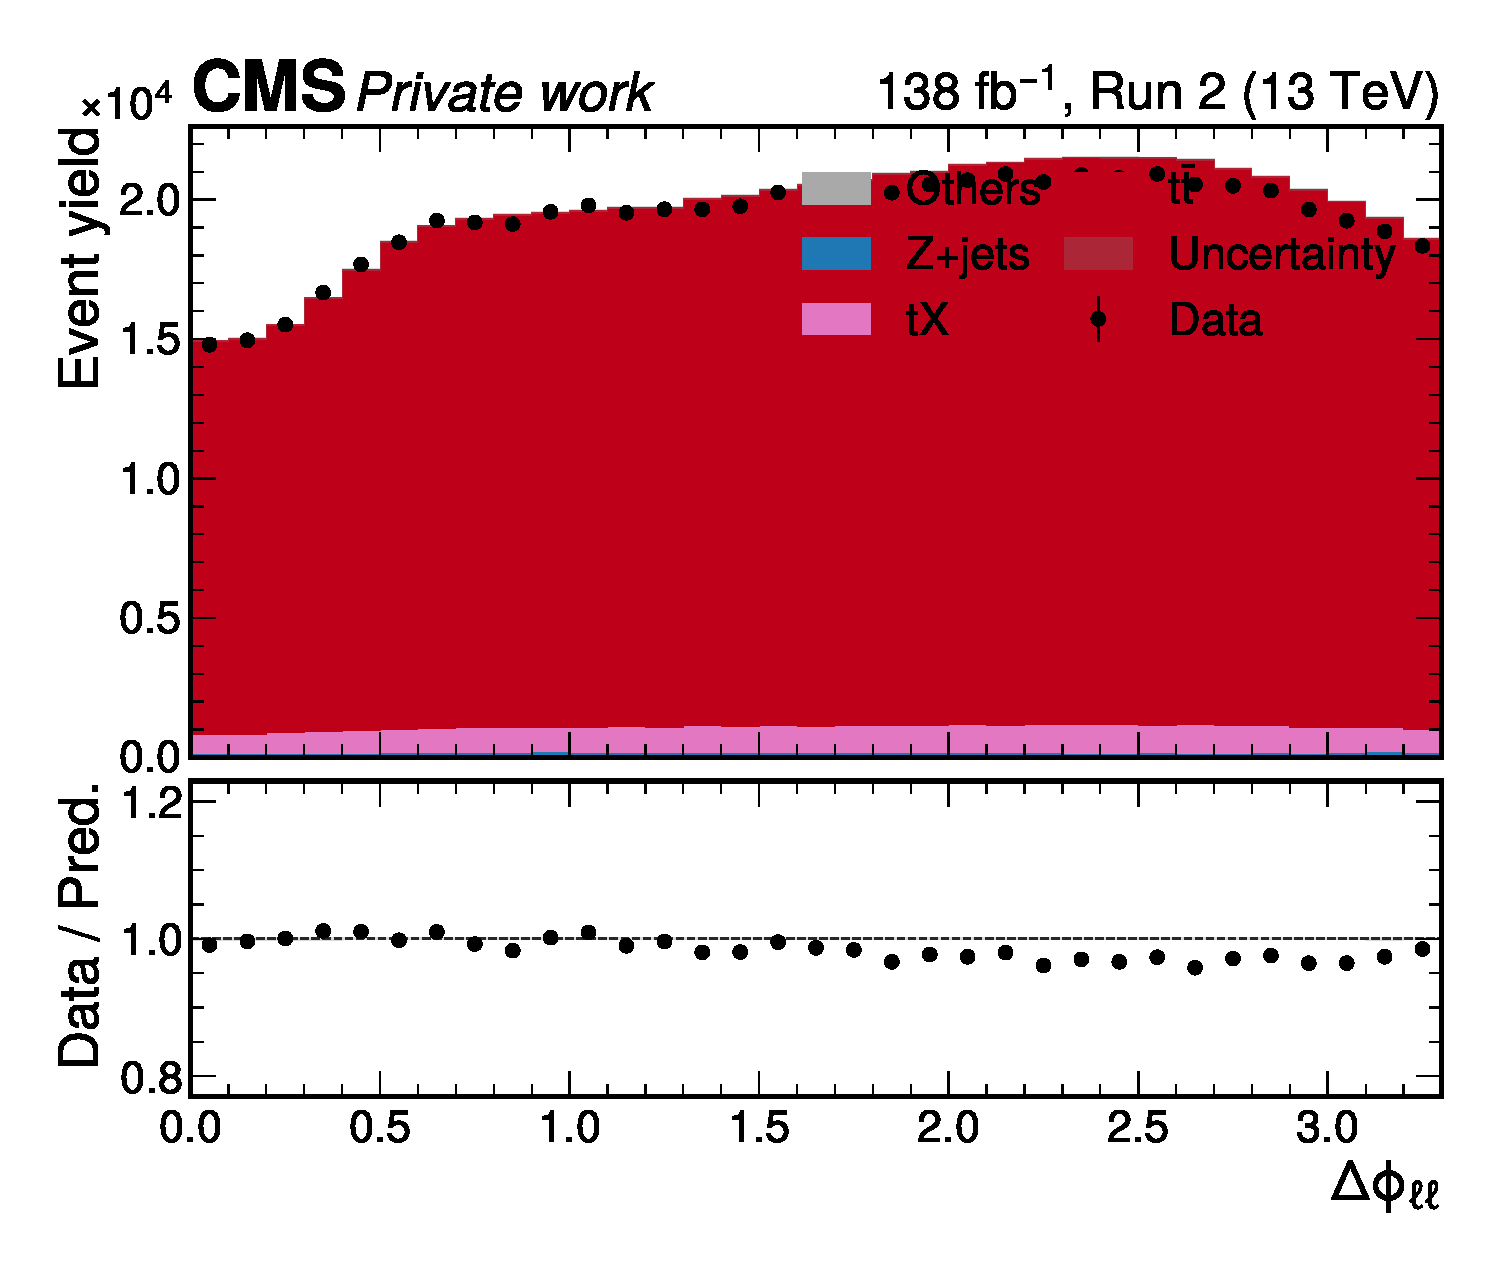
\includegraphics[width=0.49\textwidth]{figures/ah/controlplots/Req MET/em/deltaphi_Req MET_em.pdf}
    \caption{
        \textbf{Control distributions.} Shown are the distributions of \pt of both leptons (top), $\eta$ of both leptons (center), and the azimuthal angle \dphill between the leptons (bottom) in the \ee/\mumu (left) and \emu channels (right). All figures show both data (black dots) and different simulated background processes (colored bars), as well as the statistical uncertainty only. 
    }
    \label{fig:ah:control1}
\end{figure}

\begin{figure}[!p]
    \centering
    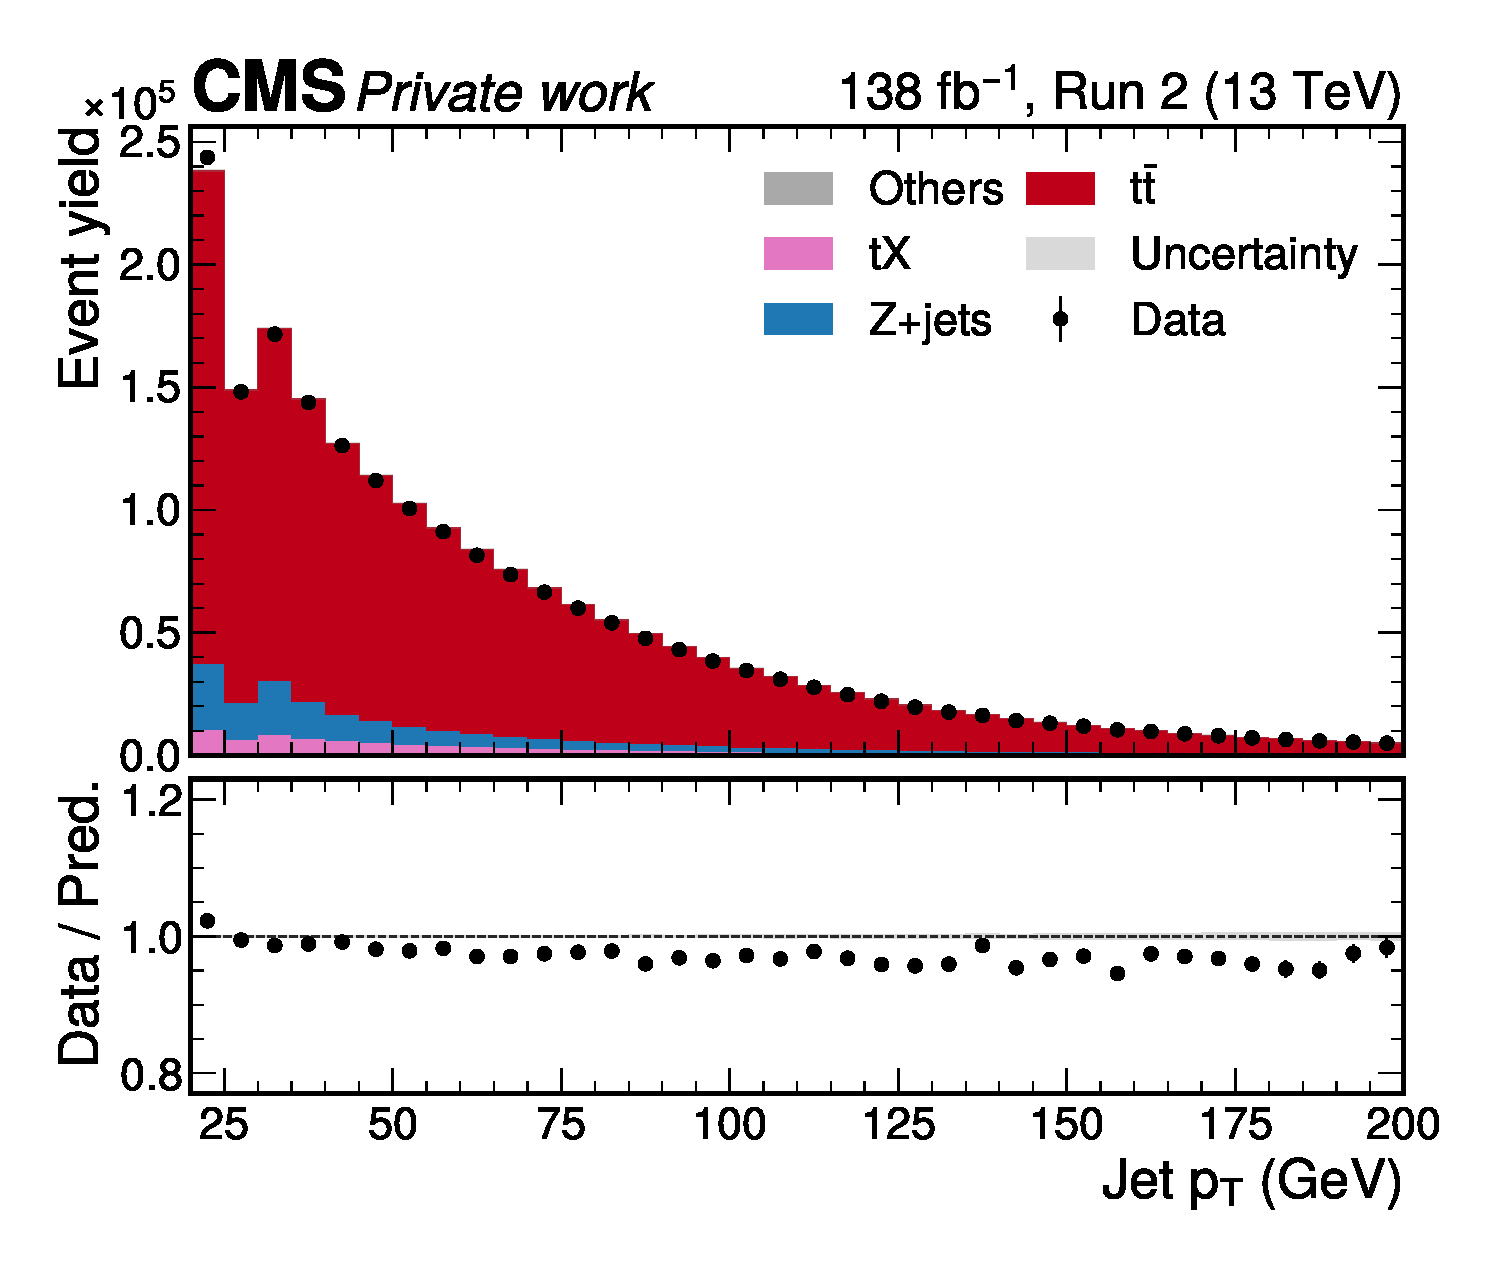
\includegraphics[width=0.49\textwidth]{figures/ah/controlplots/Req MET/sf/Jetpt_Req MET_sf.pdf}
    \hfill
    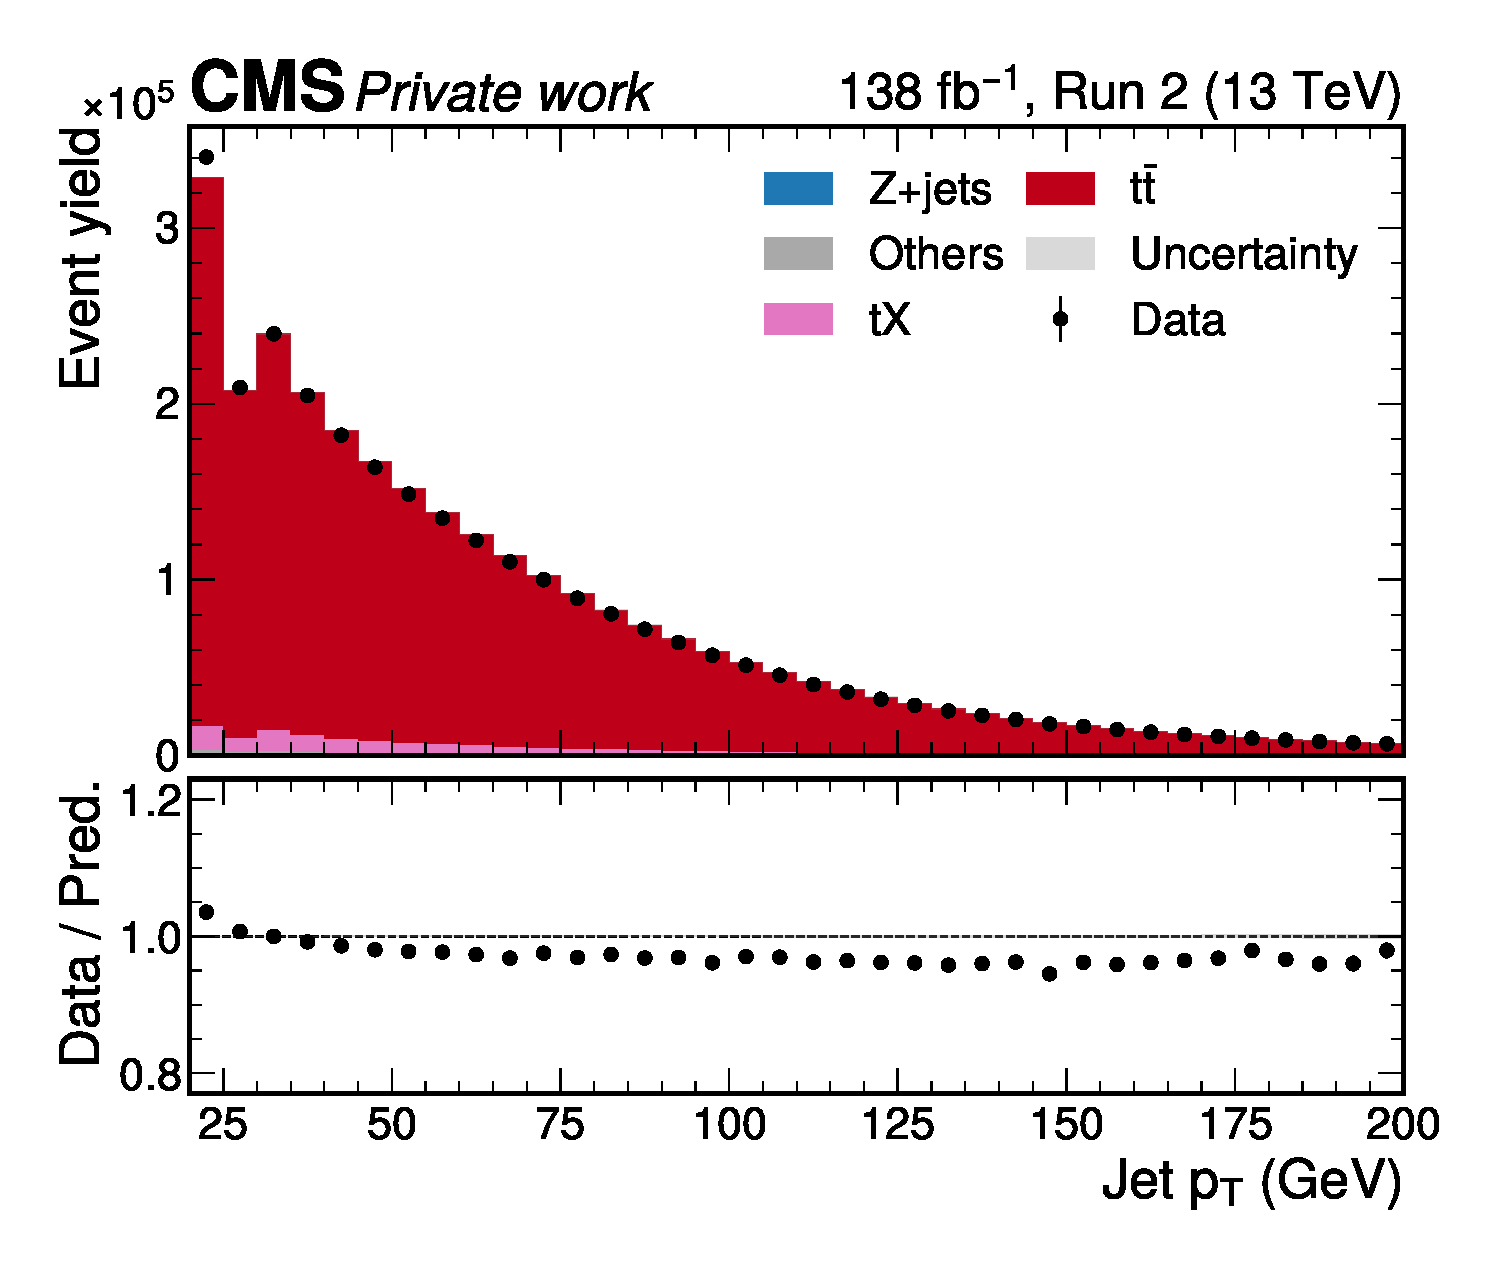
\includegraphics[width=0.49\textwidth]{figures/ah/controlplots/Req MET/em/Jetpt_Req MET_em.pdf}
    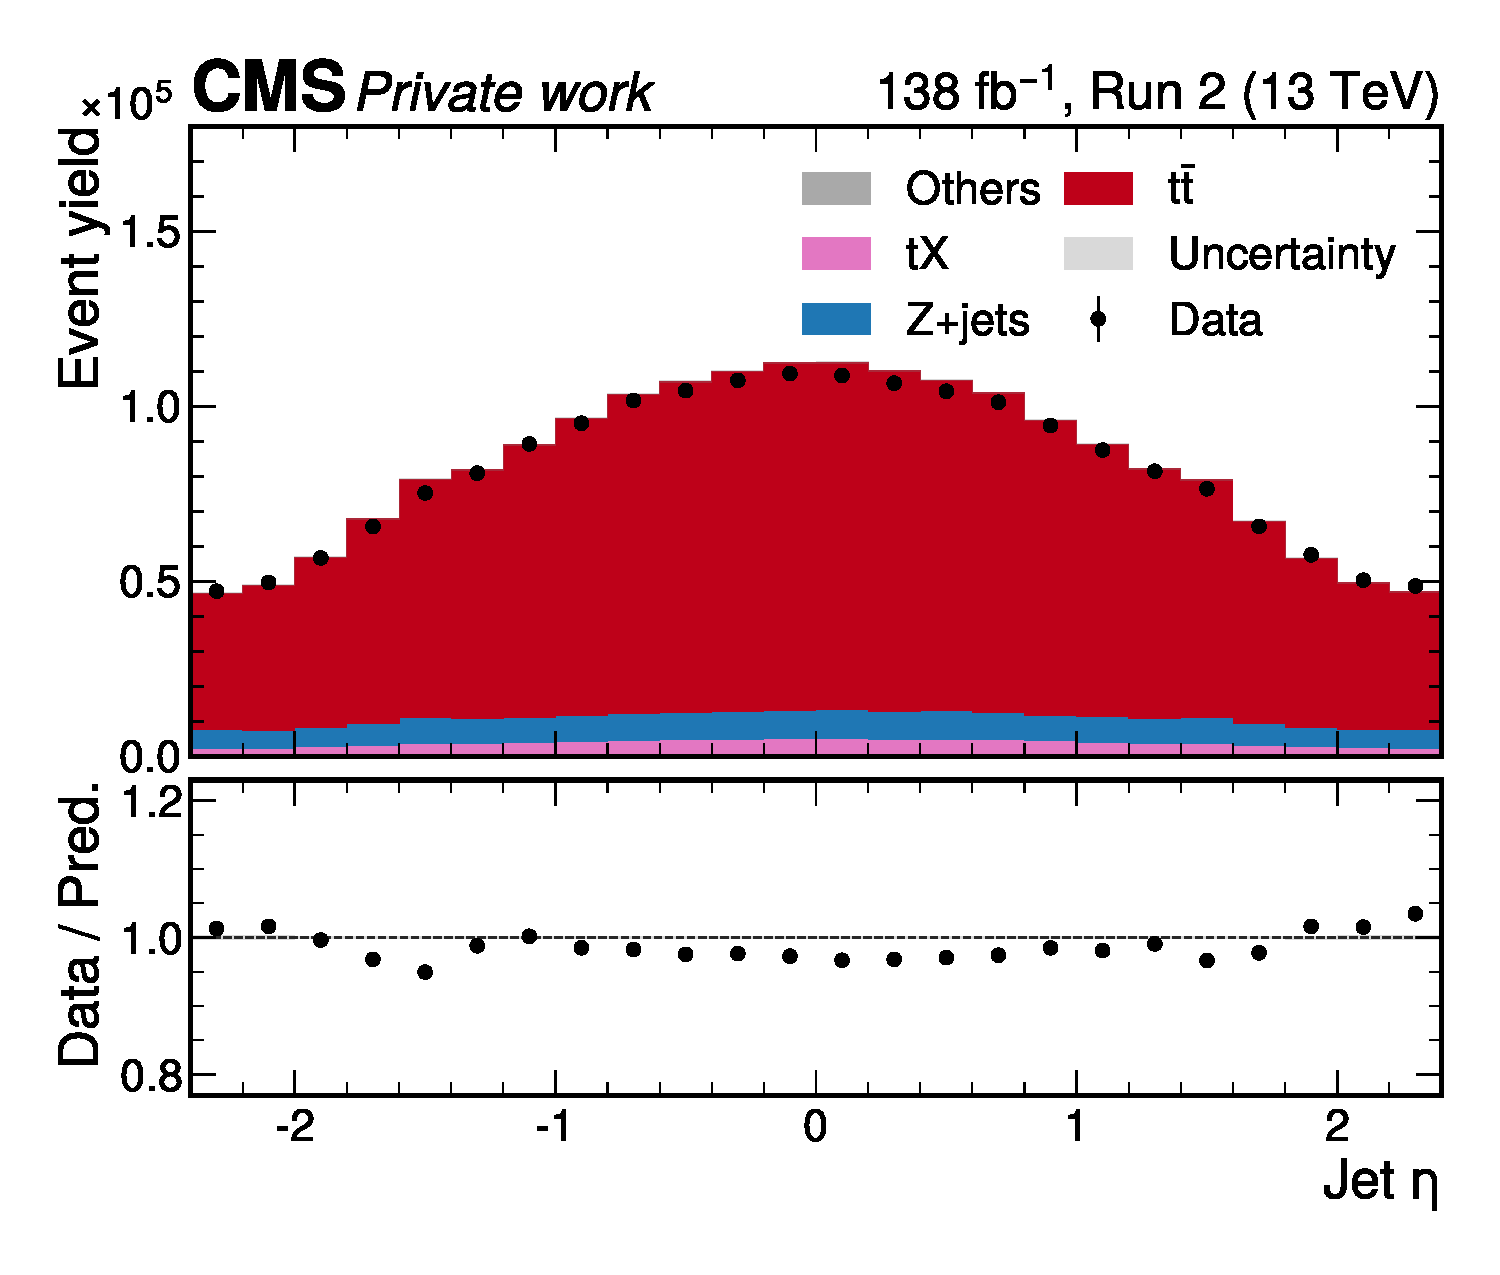
\includegraphics[width=0.49\textwidth]{figures/ah/controlplots/Req MET/sf/Jeteta_Req MET_sf.pdf}
    \hfill
    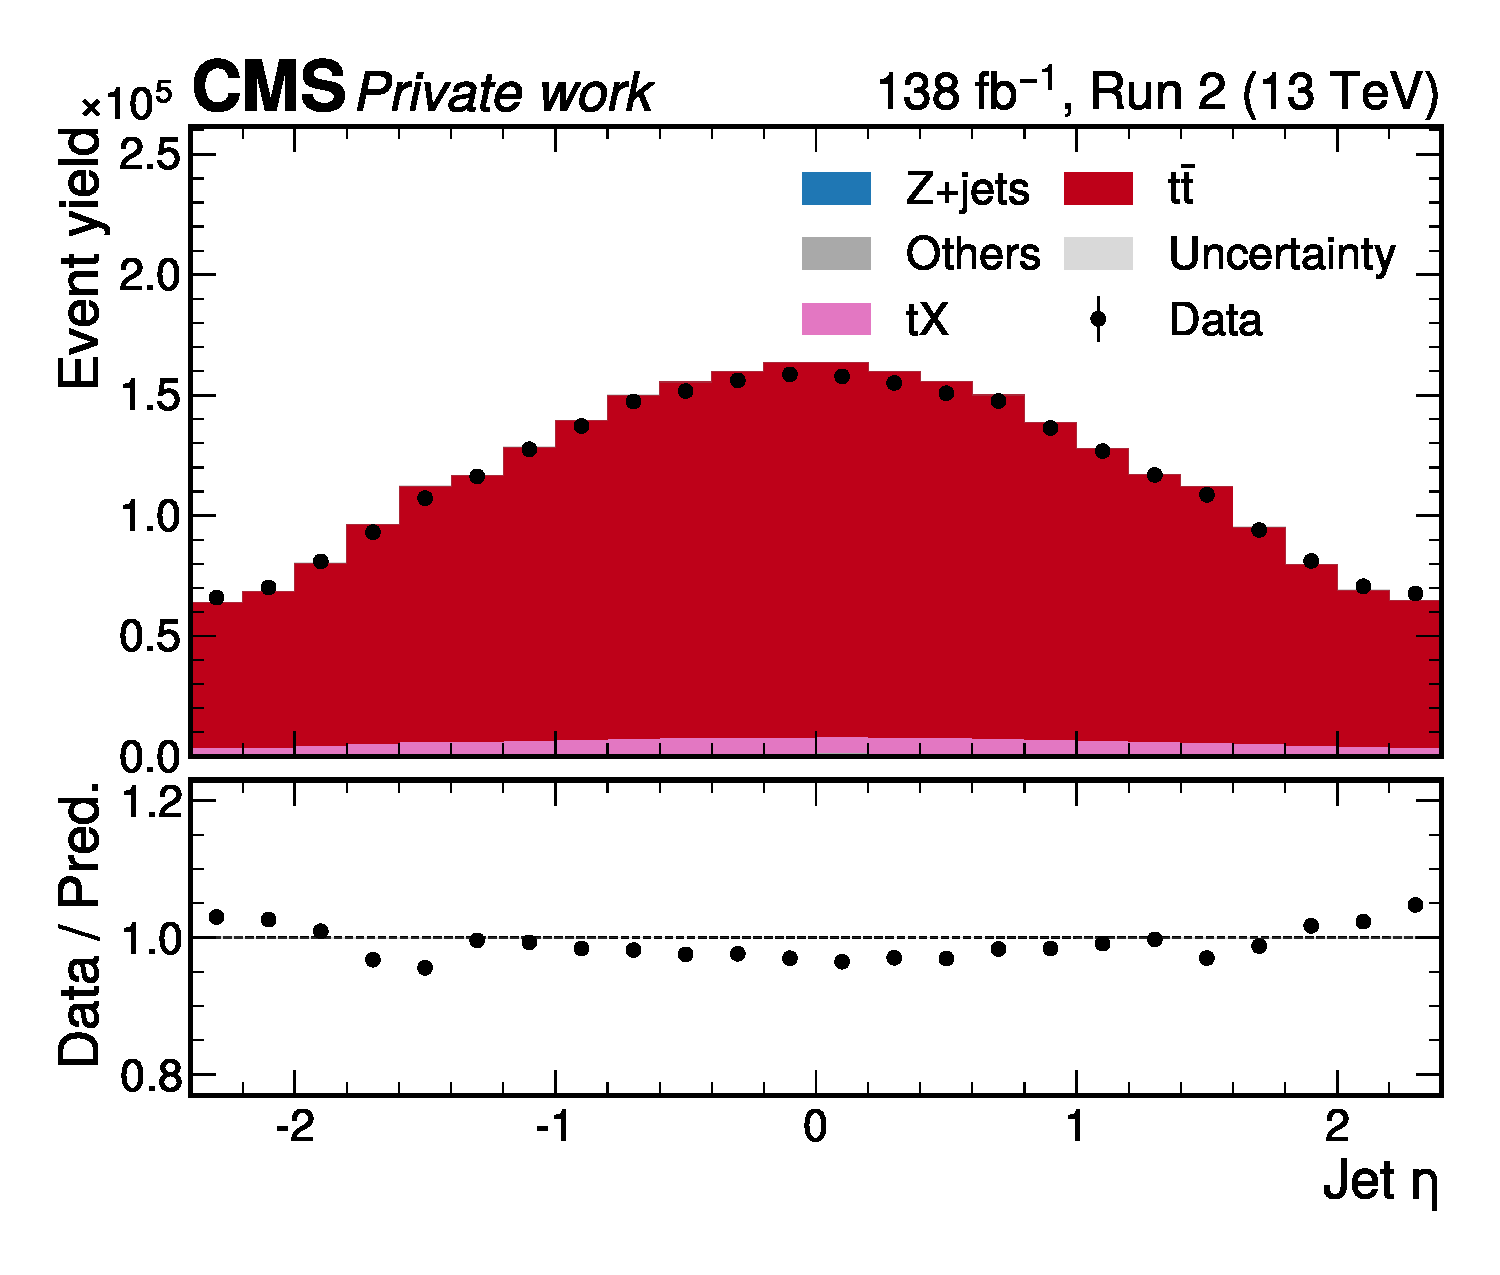
\includegraphics[width=0.49\textwidth]{figures/ah/controlplots/Req MET/em/Jeteta_Req MET_em.pdf}
    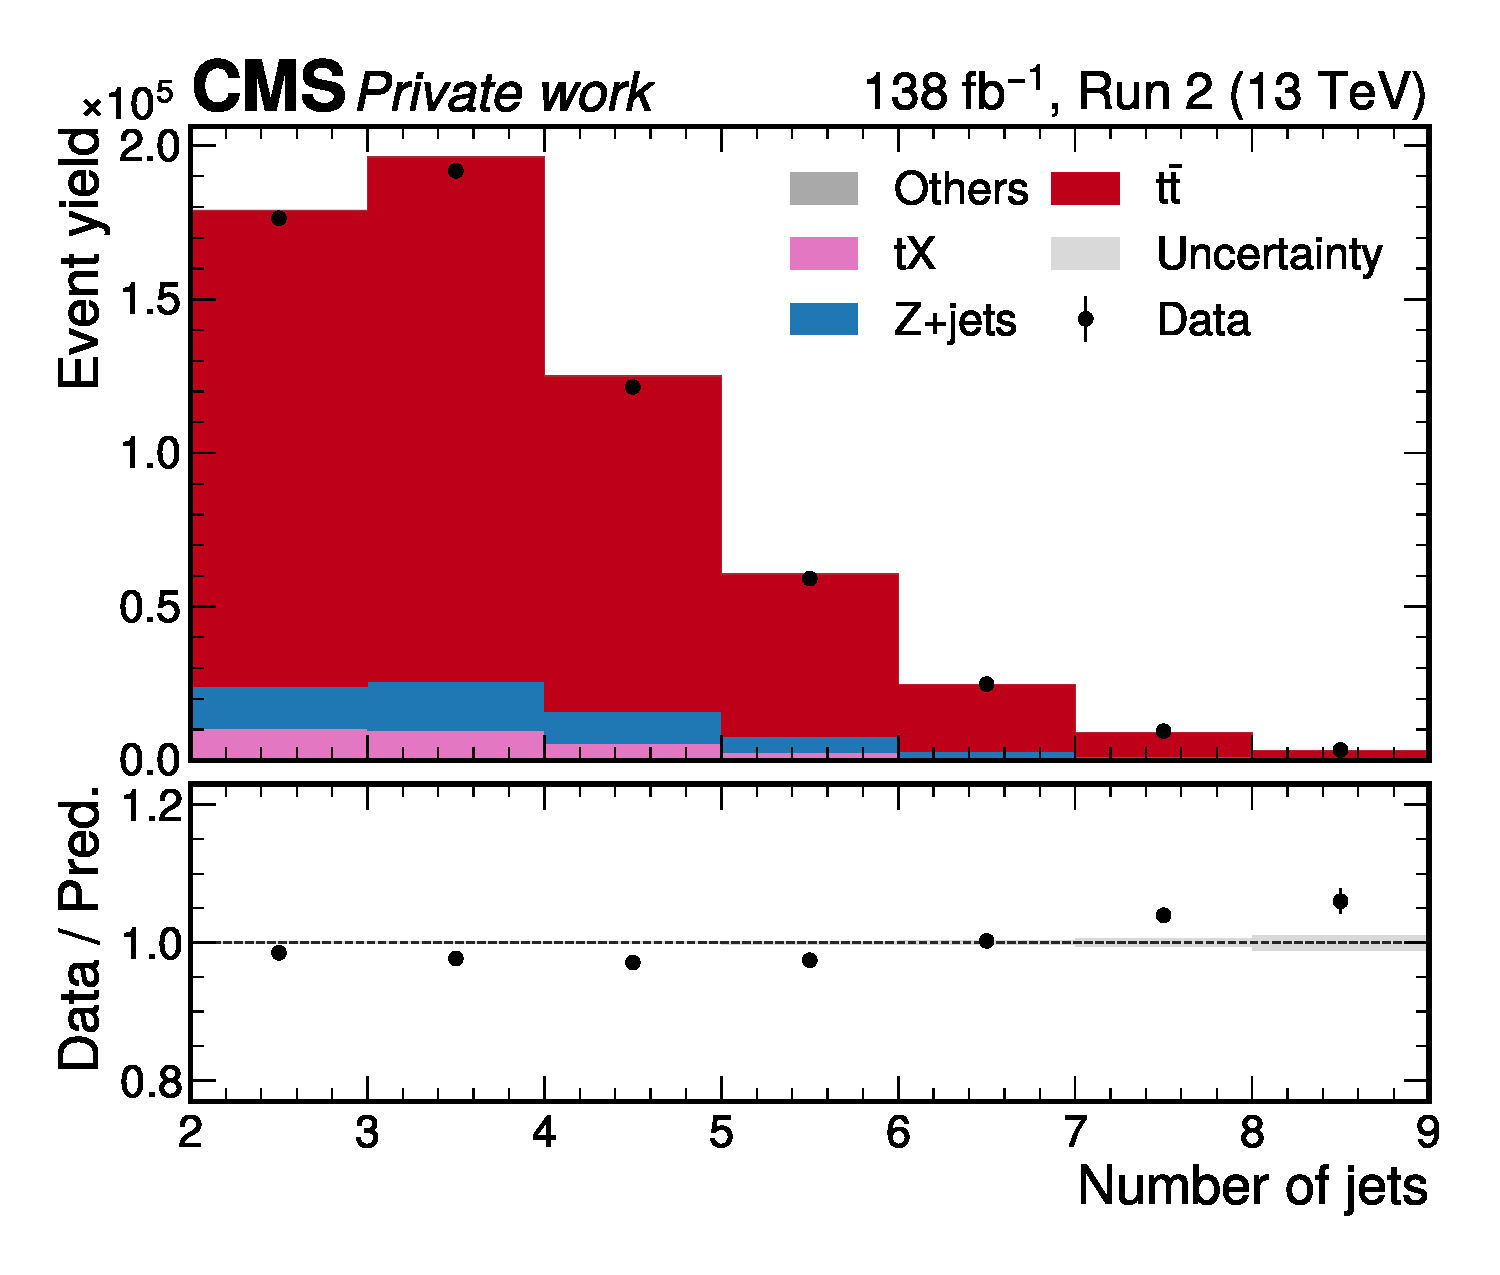
\includegraphics[width=0.49\textwidth]{figures/ah/controlplots/Req MET/sf/njet_Req MET_sf.pdf}
    \hfill
    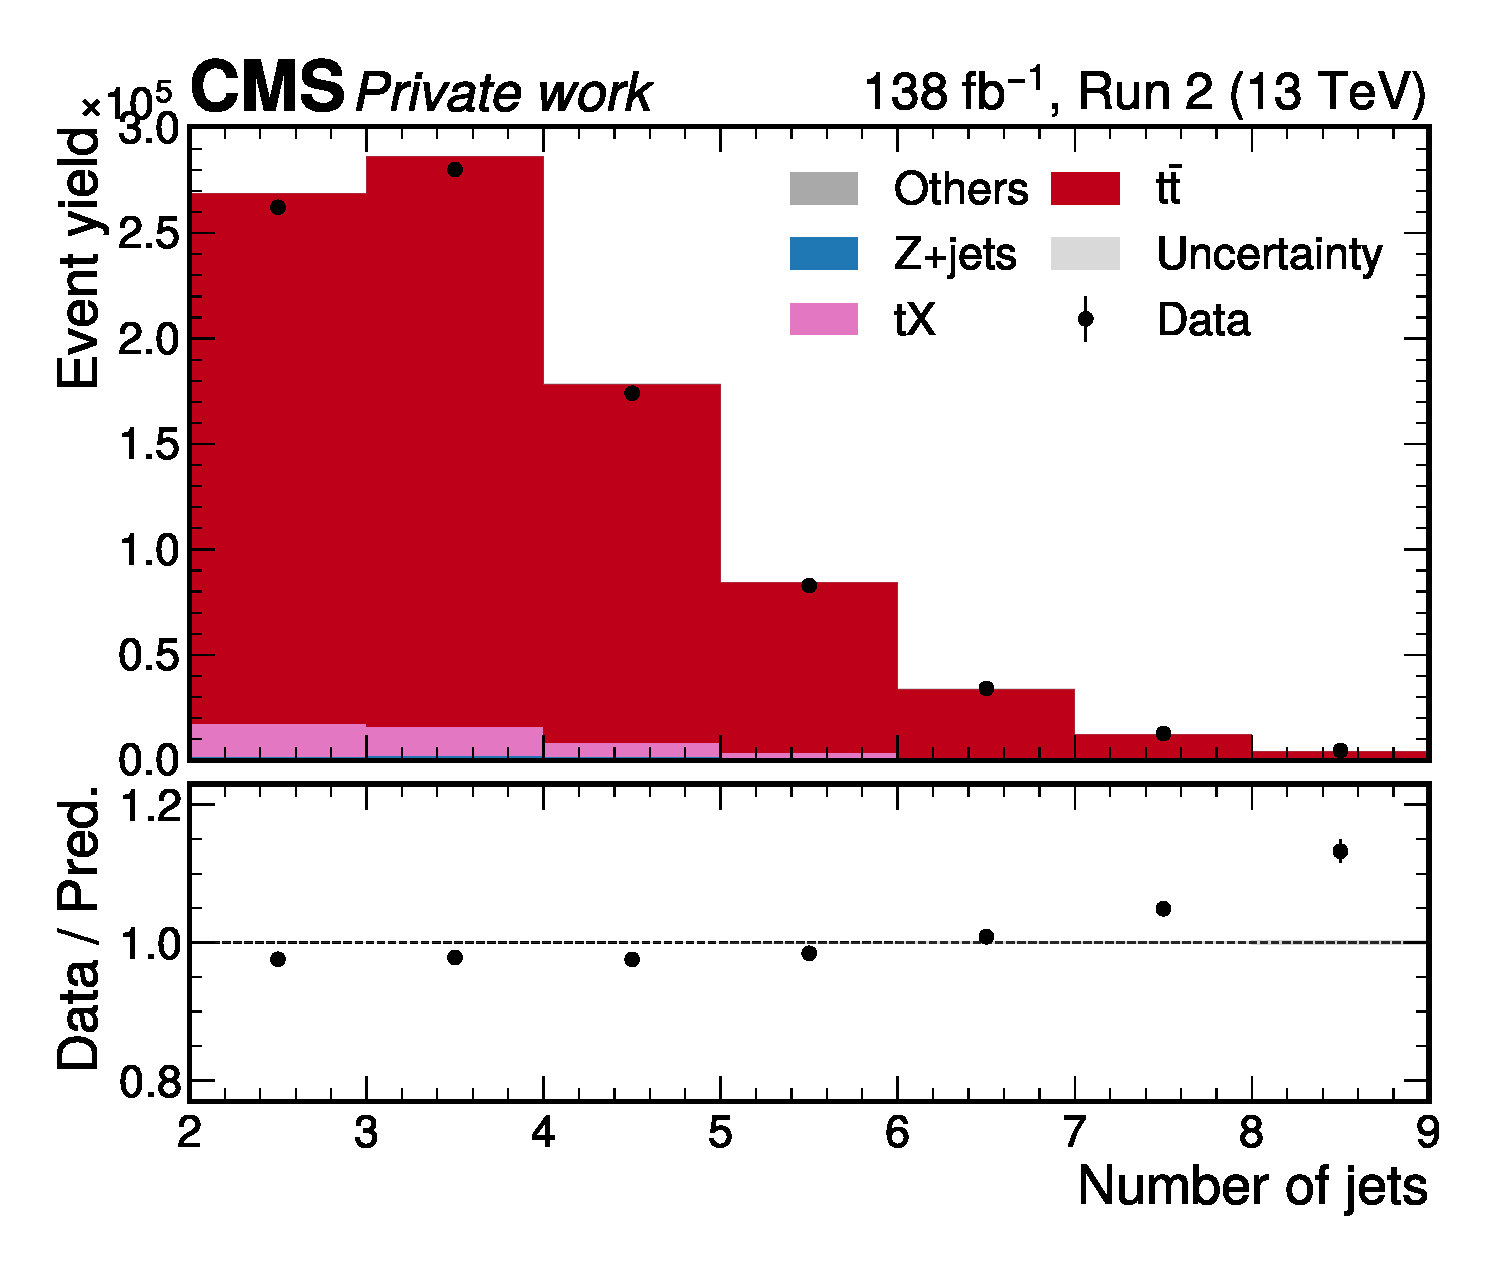
\includegraphics[width=0.49\textwidth]{figures/ah/controlplots/Req MET/em/njet_Req MET_em.pdf}
    \caption{
        \textbf{Control distributions.} Shown are the distributions of \pt of all jets (top), $\eta$ of all jets (center), and the number of jets (bottom) in the \ee/\mumu (left) and \emu channels (right). All figures show both data (black dots) and different simulated background processes (colored bars), as well as the statistical uncertainty only. 
    }
    \label{fig:ah:control2}
\end{figure}

\begin{figure}[!p]
    \centering
    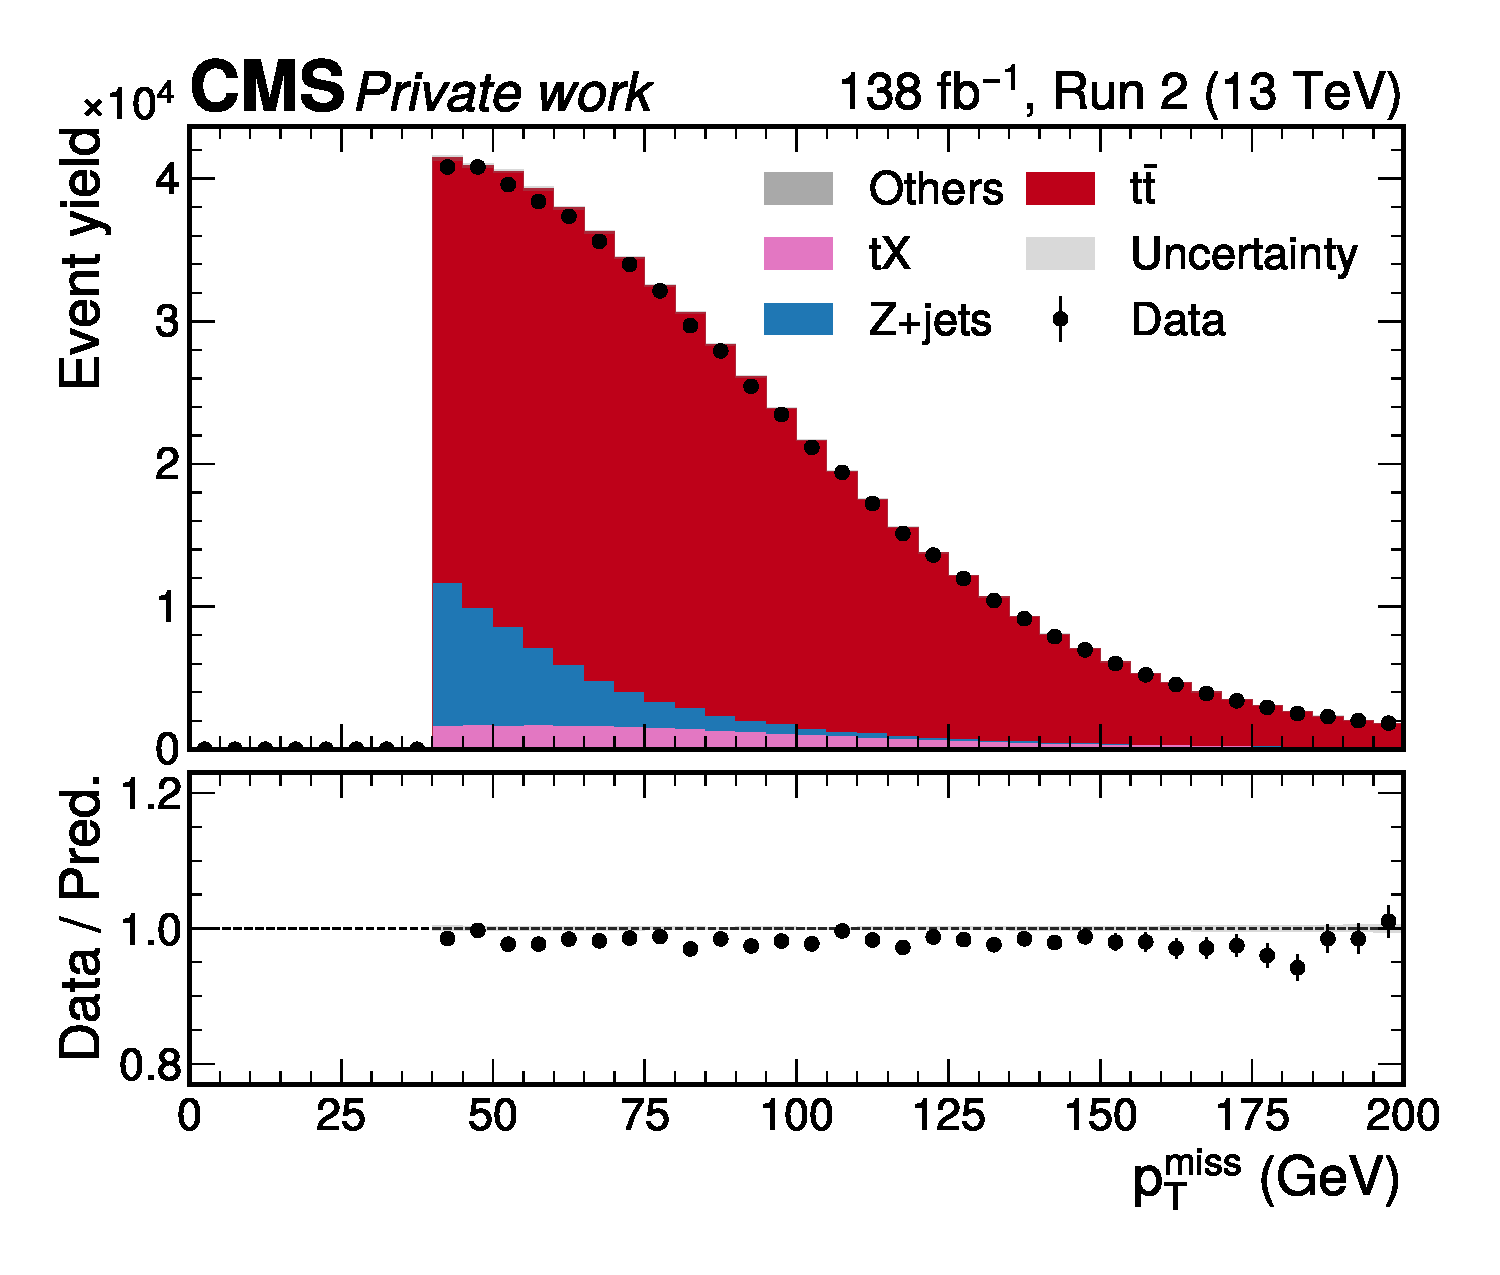
\includegraphics[width=0.49\textwidth]{figures/ah/controlplots/Req MET/sf/METpt_Req MET_sf.pdf}
    \hfill
    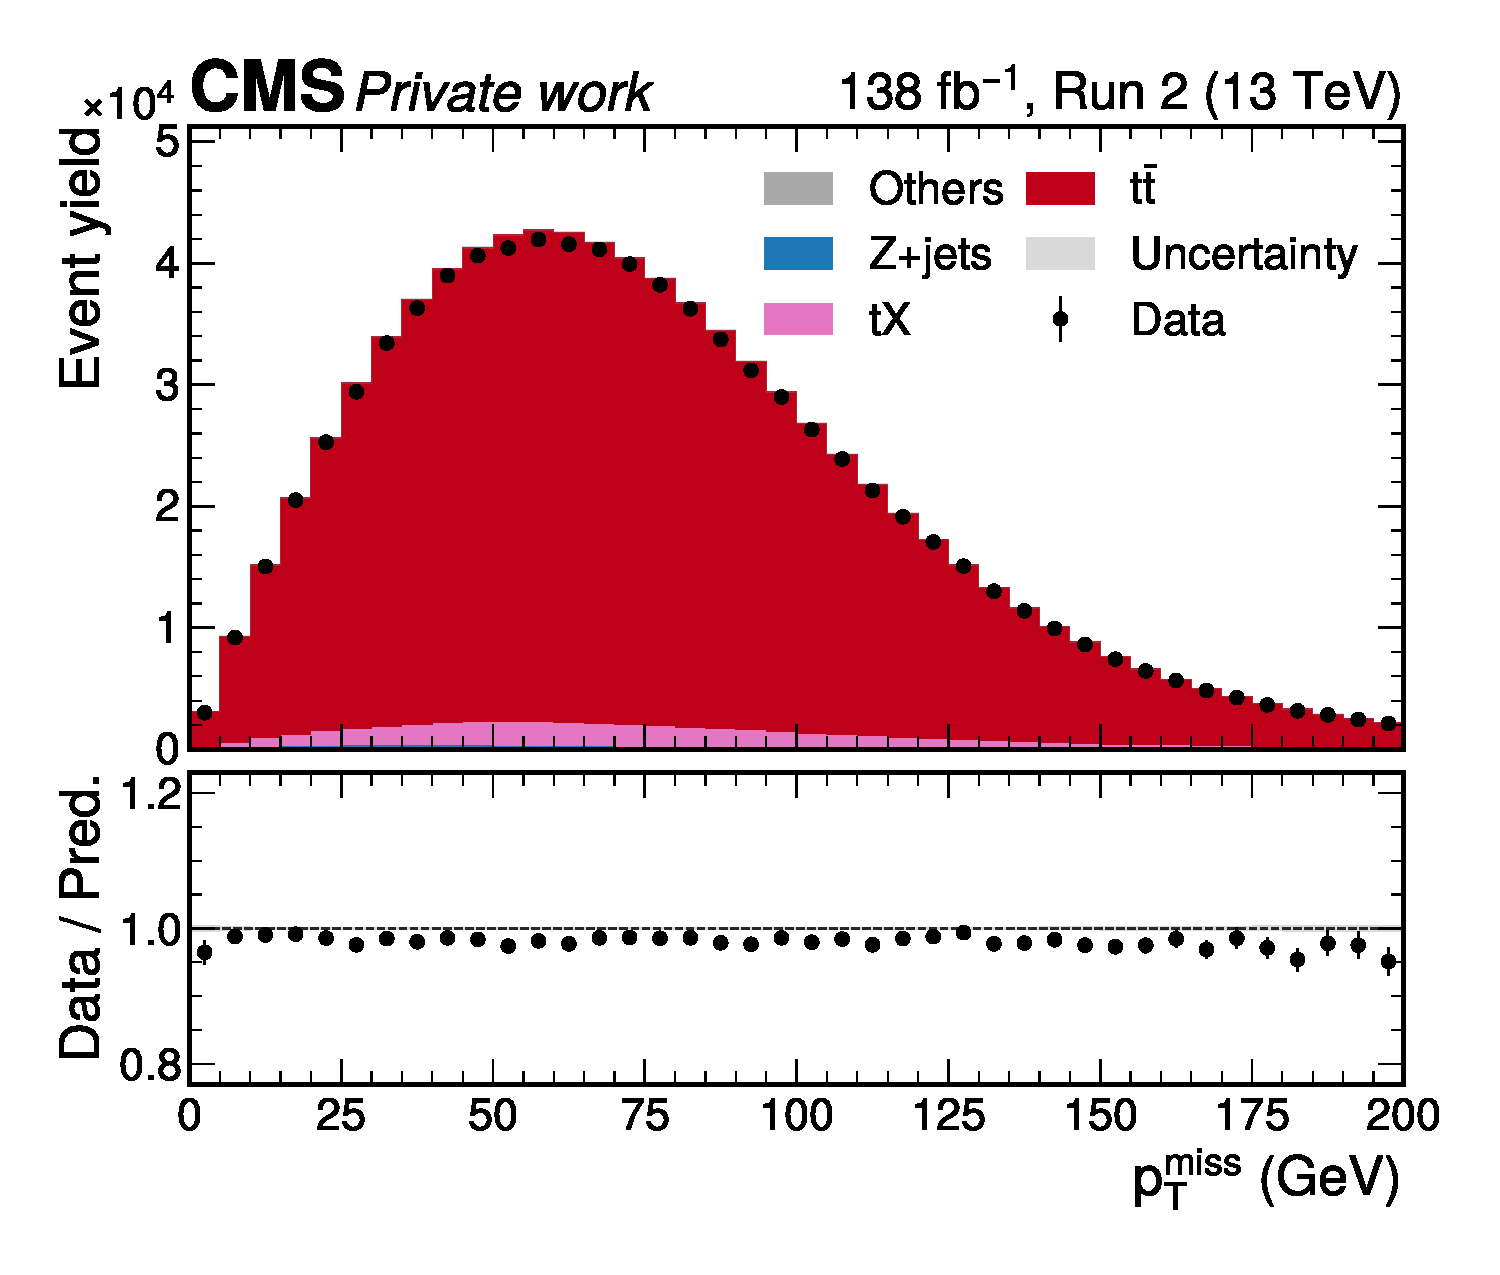
\includegraphics[width=0.49\textwidth]{figures/ah/controlplots/Req MET/em/METpt_Req MET_em.pdf}
    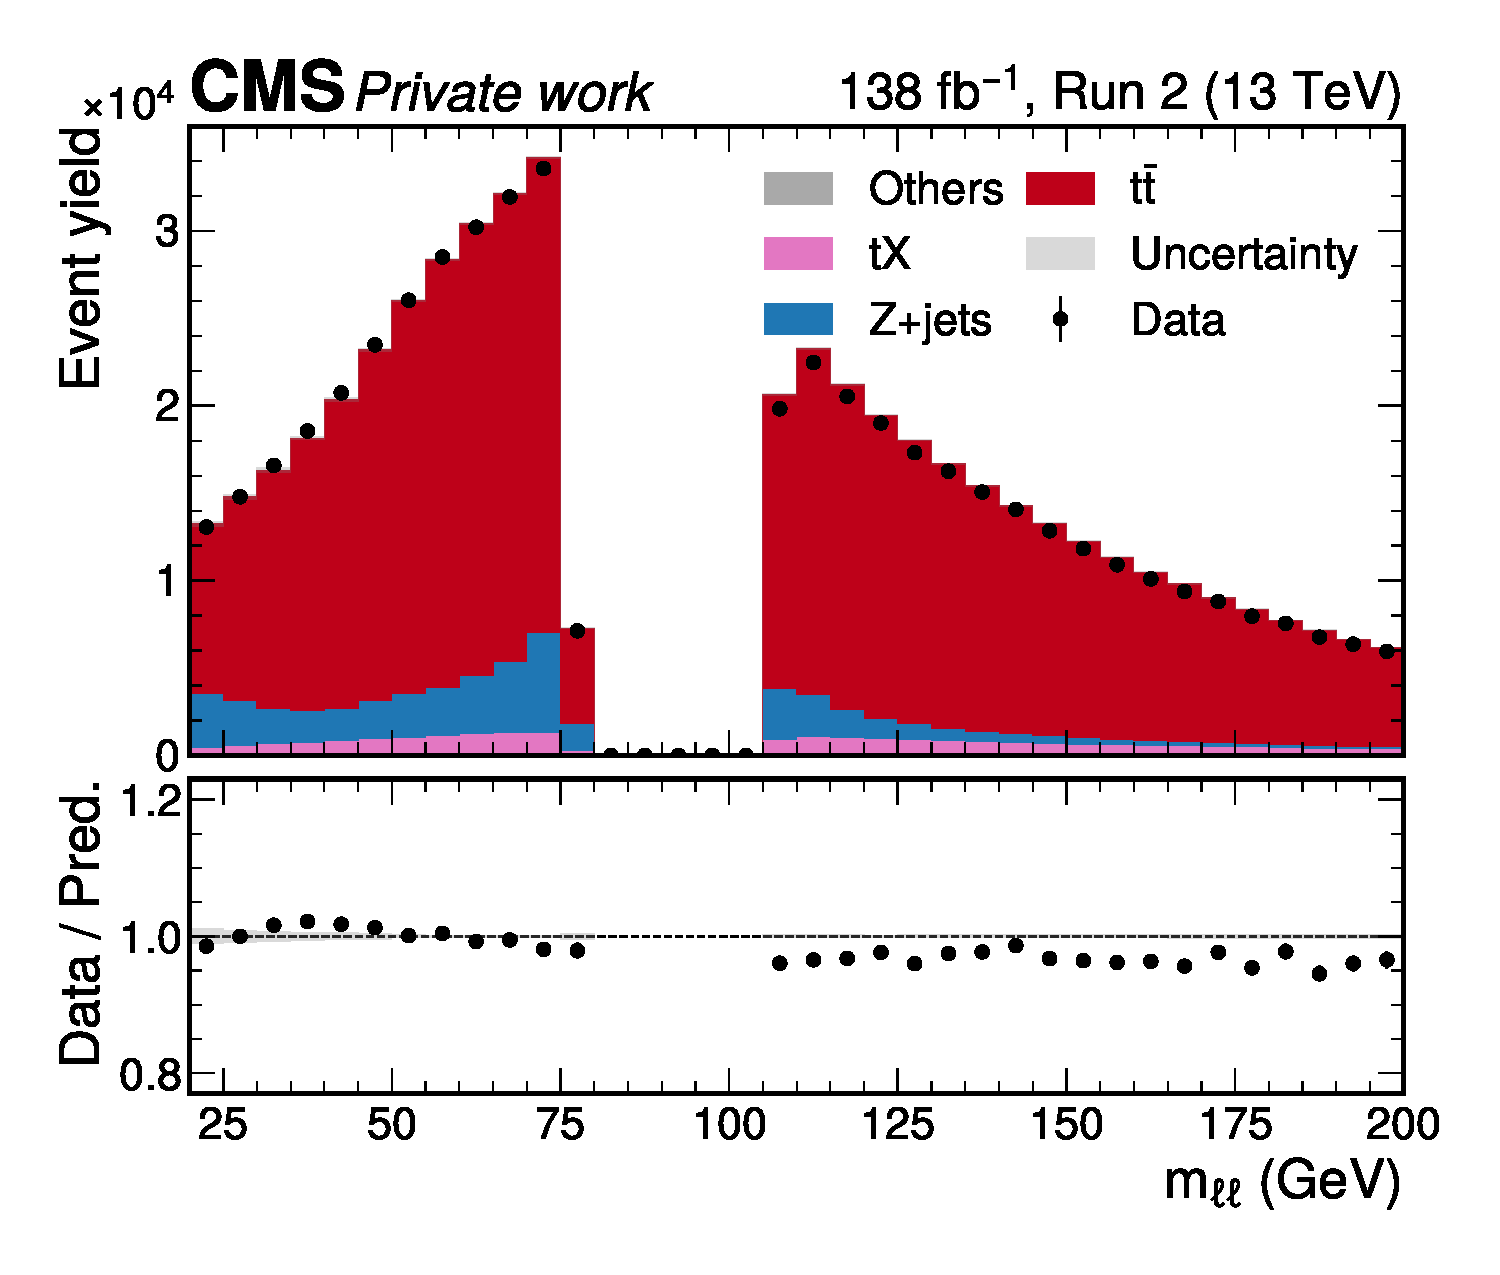
\includegraphics[width=0.49\textwidth]{figures/ah/controlplots/Req MET/sf/mll_Req MET_sf.pdf}
    \hfill
    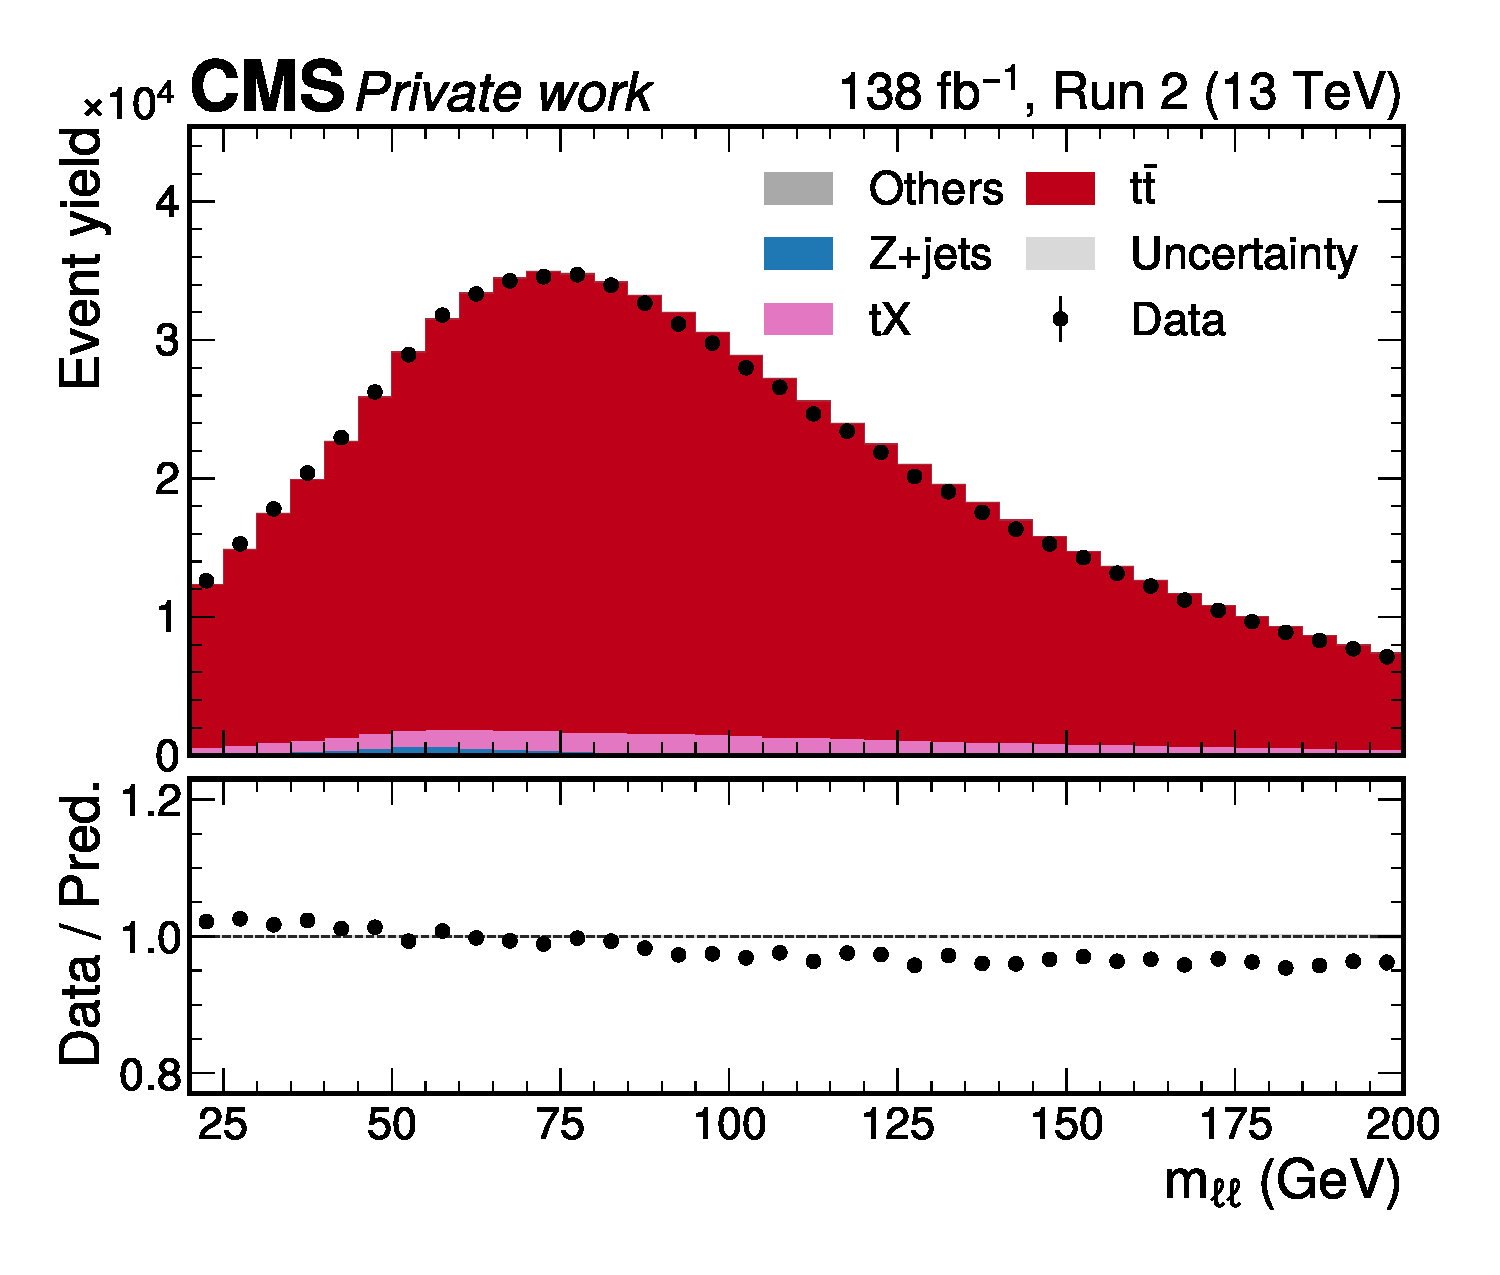
\includegraphics[width=0.49\textwidth]{figures/ah/controlplots/Req MET/em/mll_Req MET_em.pdf}
    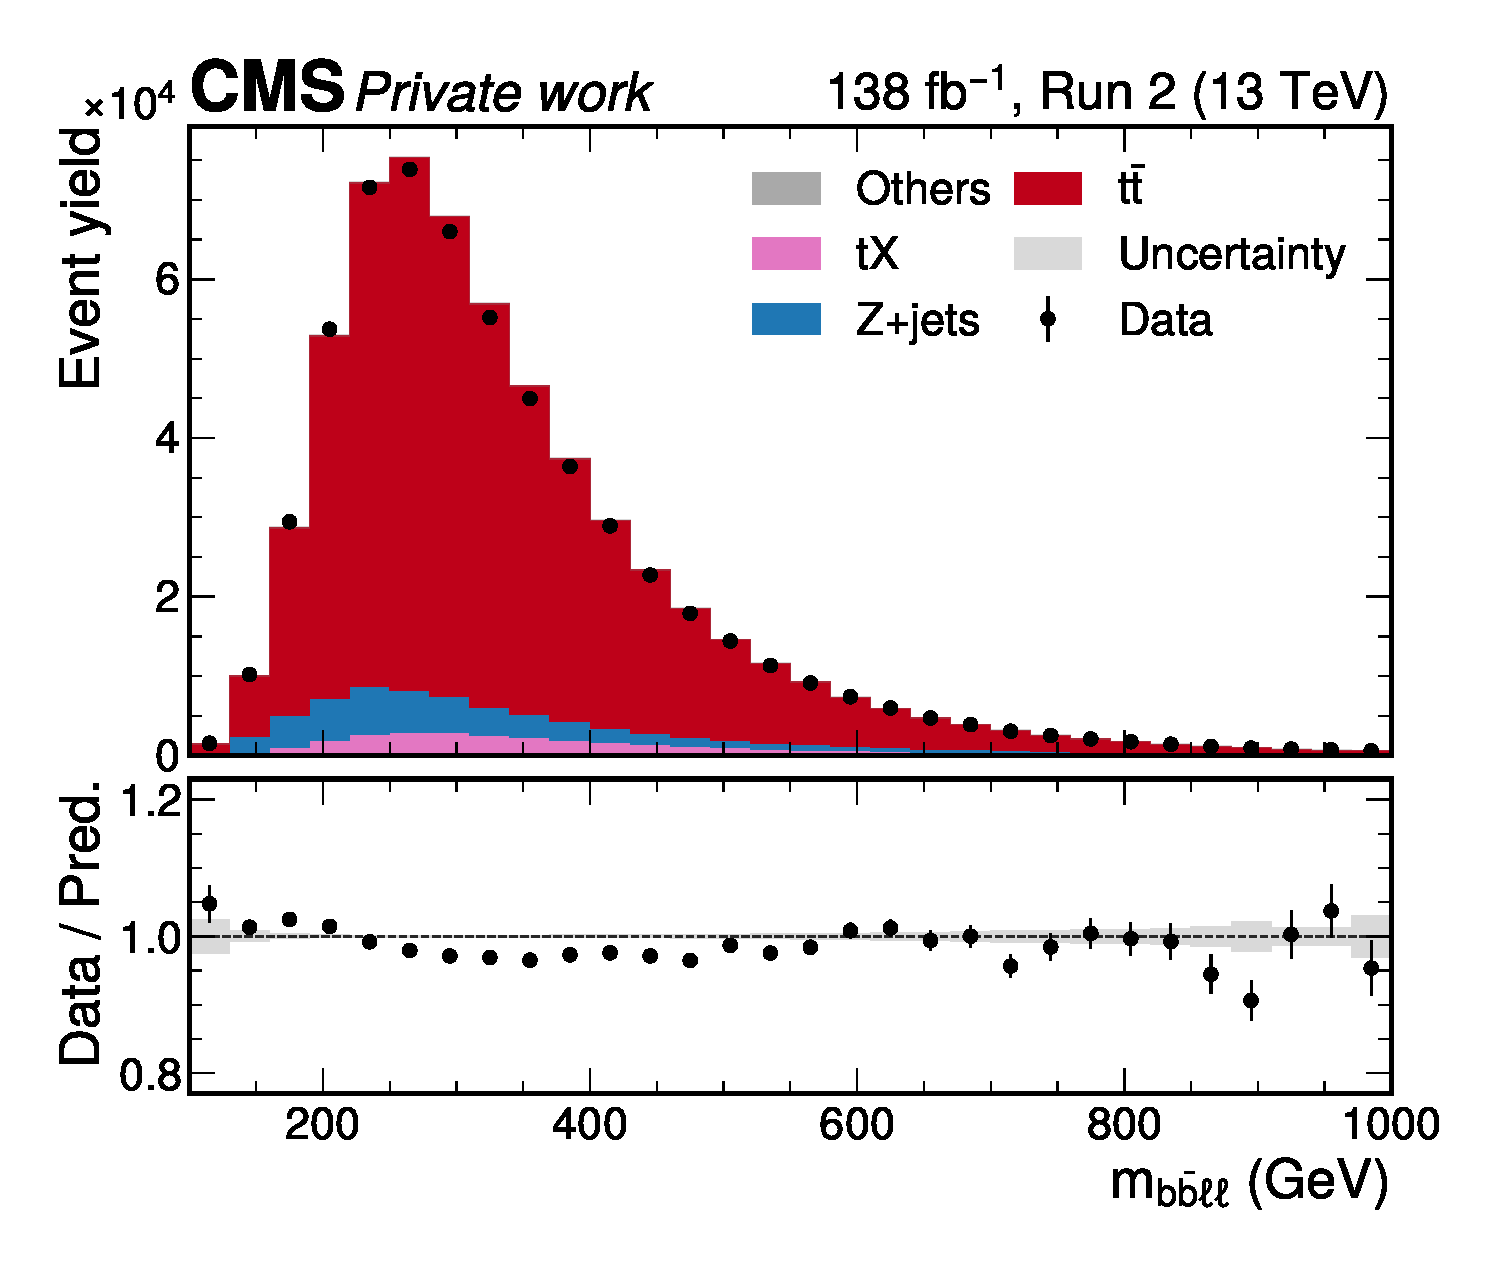
\includegraphics[width=0.49\textwidth]{figures/ah/controlplots/Reco/sf/mbbll__sf.pdf}
    \hfill
    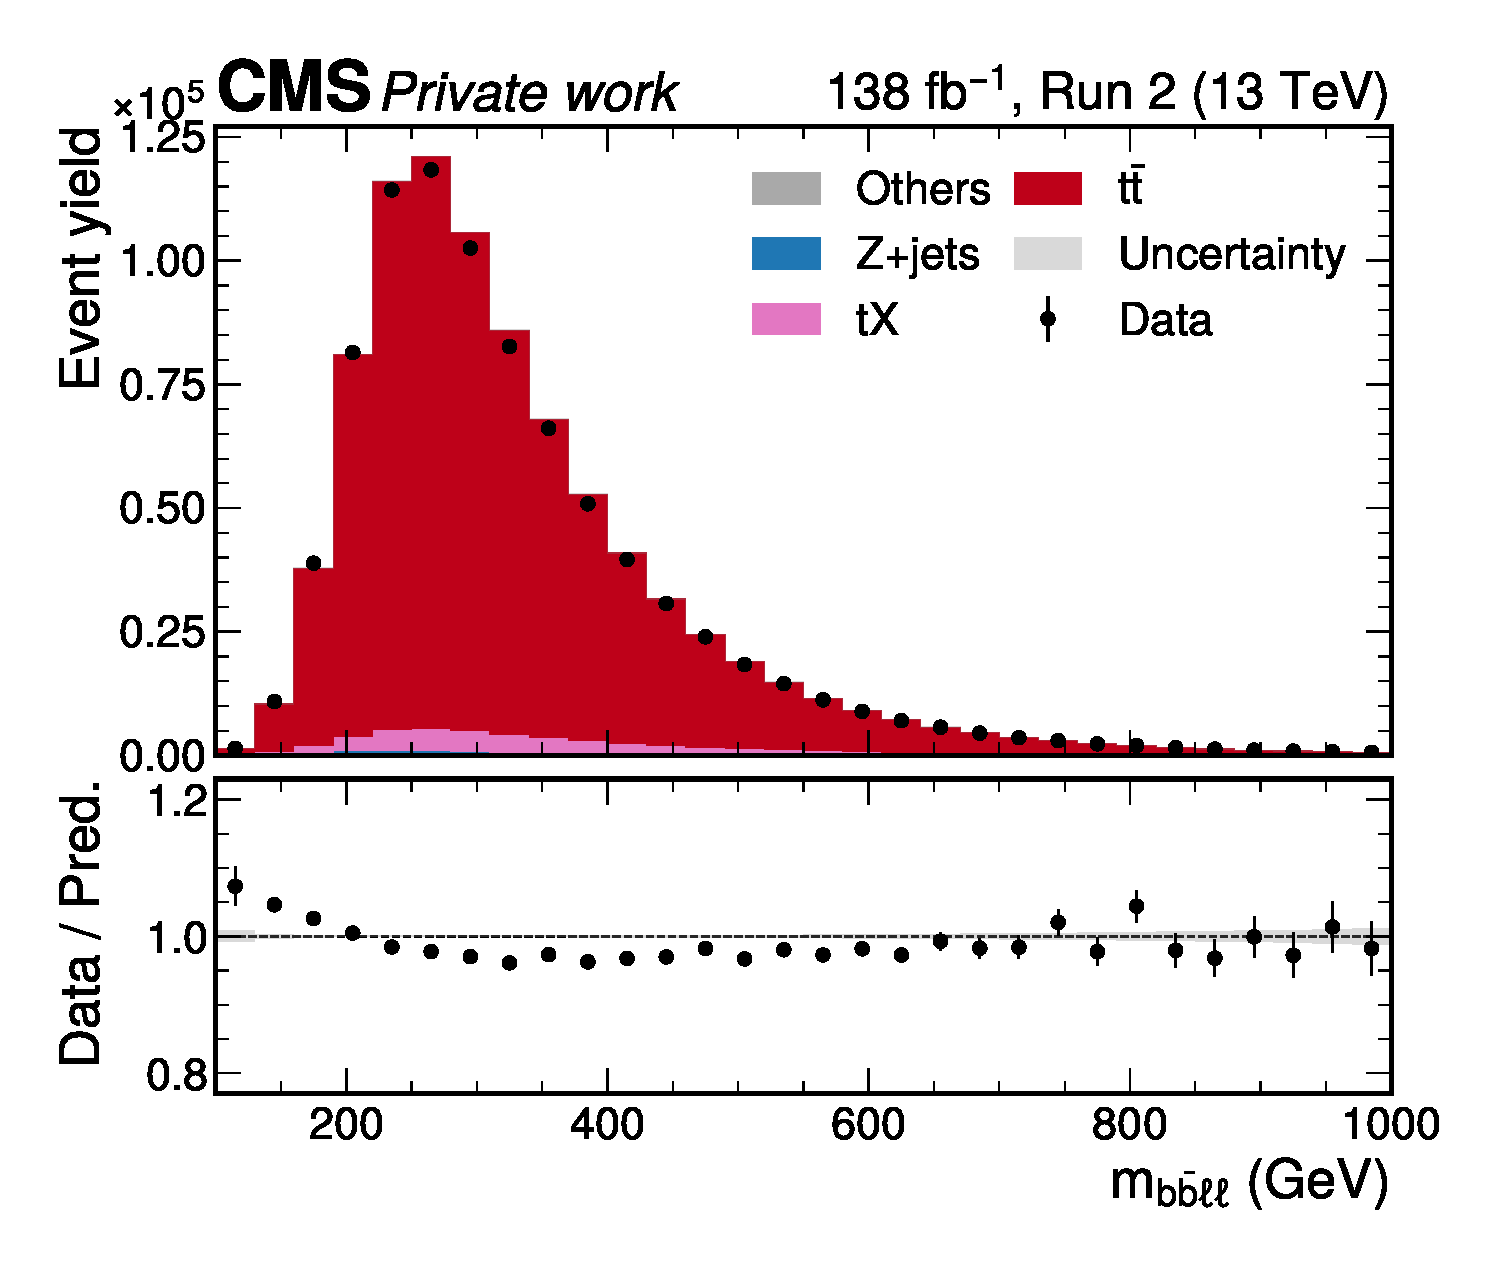
\includegraphics[width=0.49\textwidth]{figures/ah/controlplots/Reco/em/mbbll__em.pdf}
    \caption{
        \textbf{Control distributions.} Shown are the distributions of \ptmiss (top), \mll (center), and the invariant mass \mbbll of both b candidates and both leptons  (bottom) in the \ee/\mumu (left) and \emu channels (right). All figures show both data (black dots) and different simulated background processes (colored bars), as well as the statistical uncertainty only. 
    }
    \label{fig:ah:control3}
\end{figure}

\begin{figure}[!p]
    \centering
    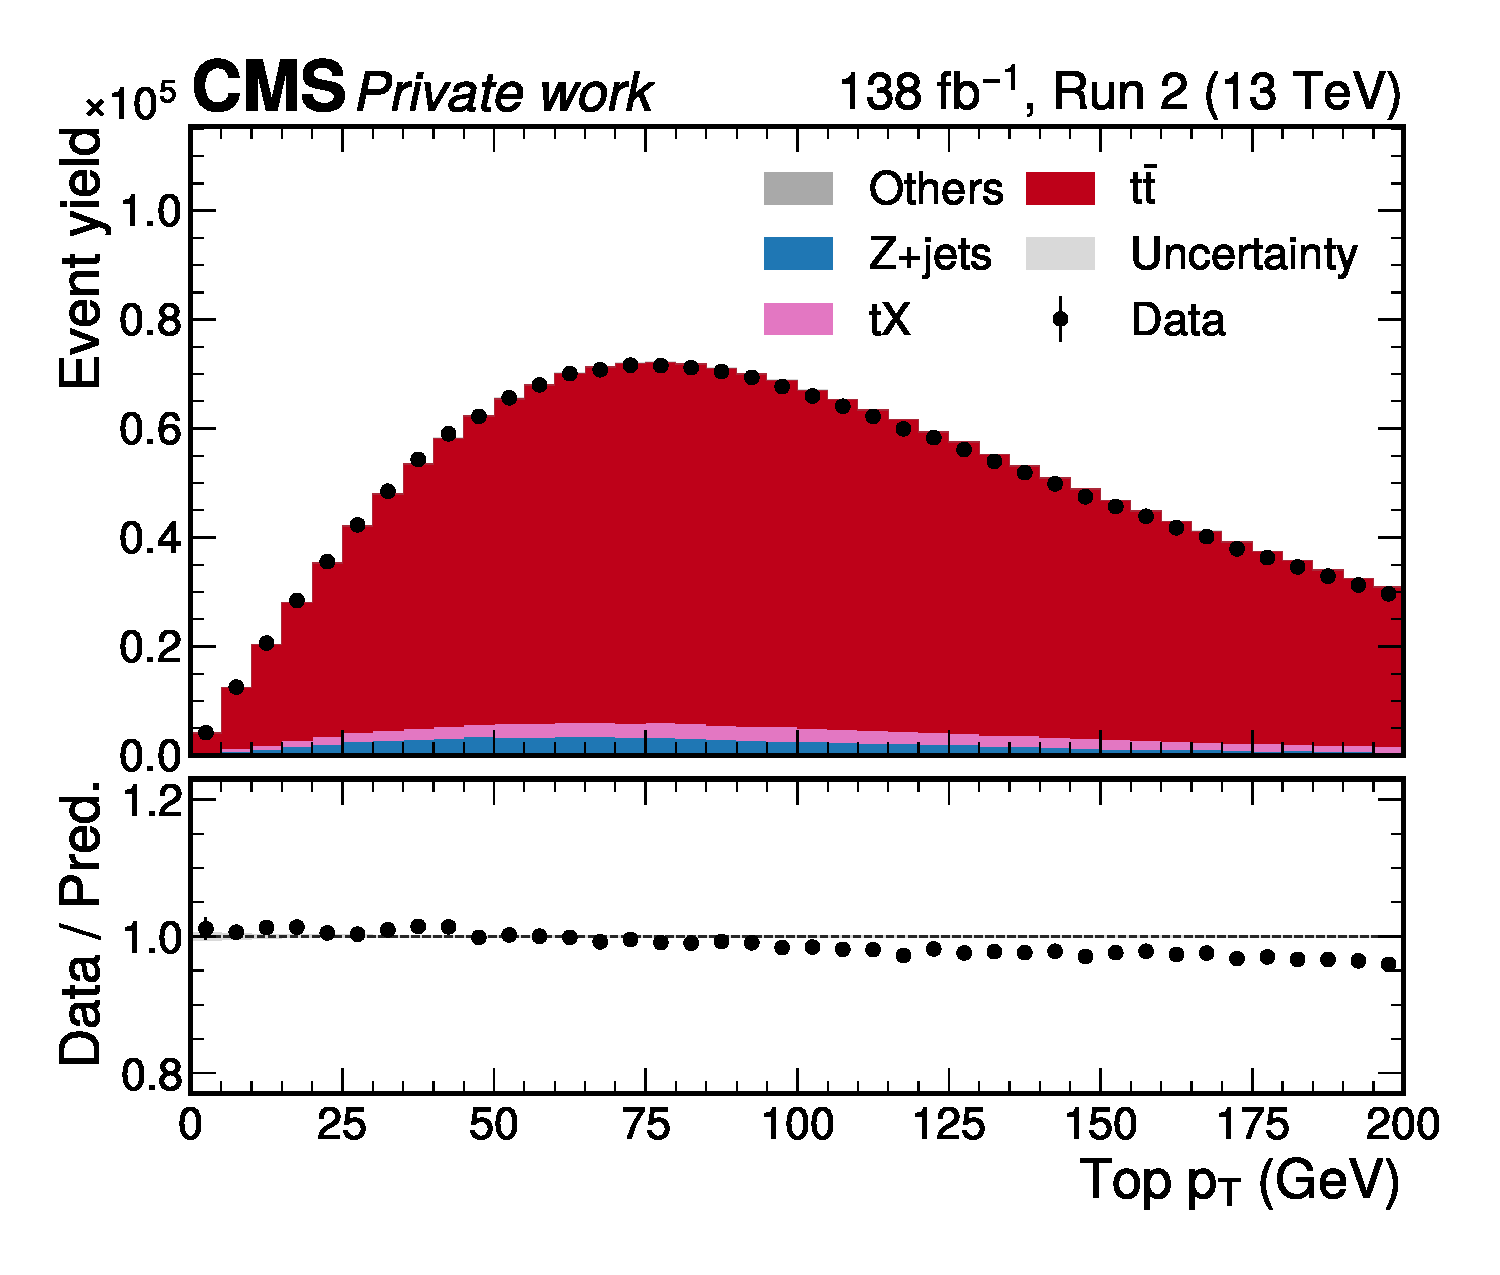
\includegraphics[width=0.49\textwidth]{figures/ah/controlplots/Reco/ll/toppt_Reco_ll.pdf}
    \hfill
    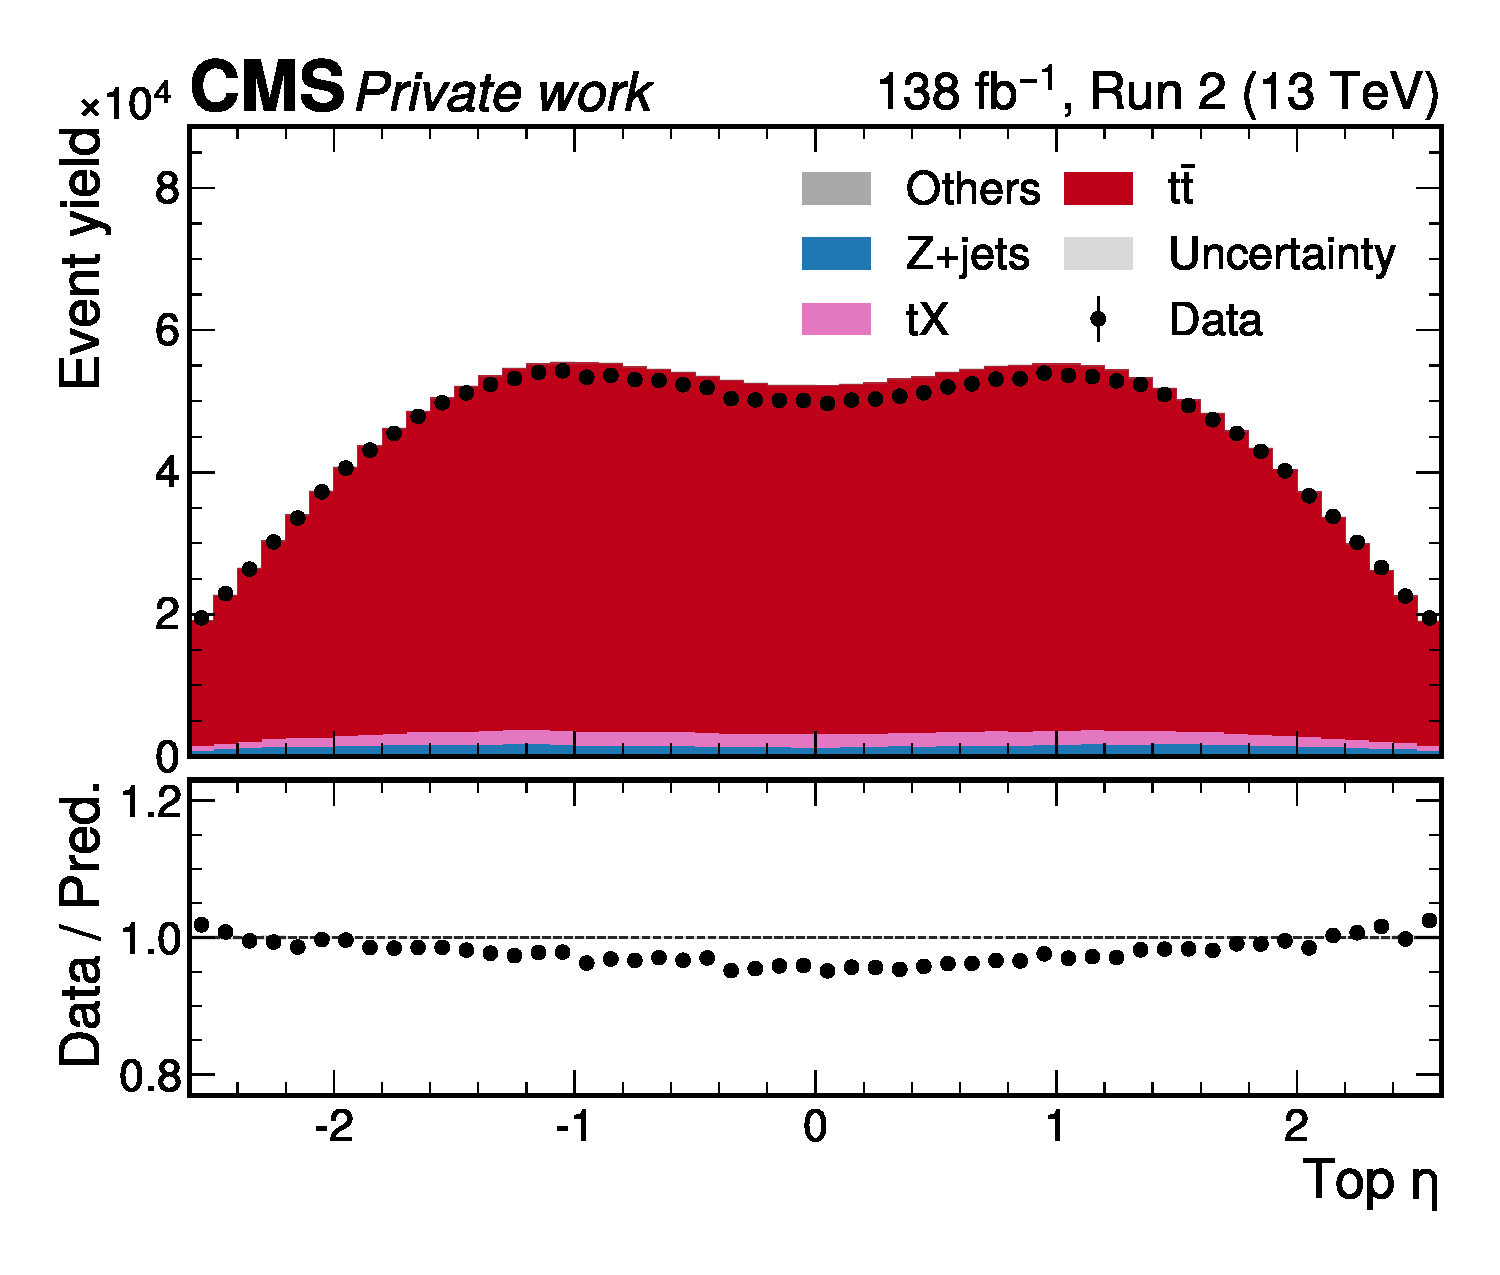
\includegraphics[width=0.49\textwidth]{figures/ah/controlplots/Reco/ll/topeta_Reco_ll.pdf}
    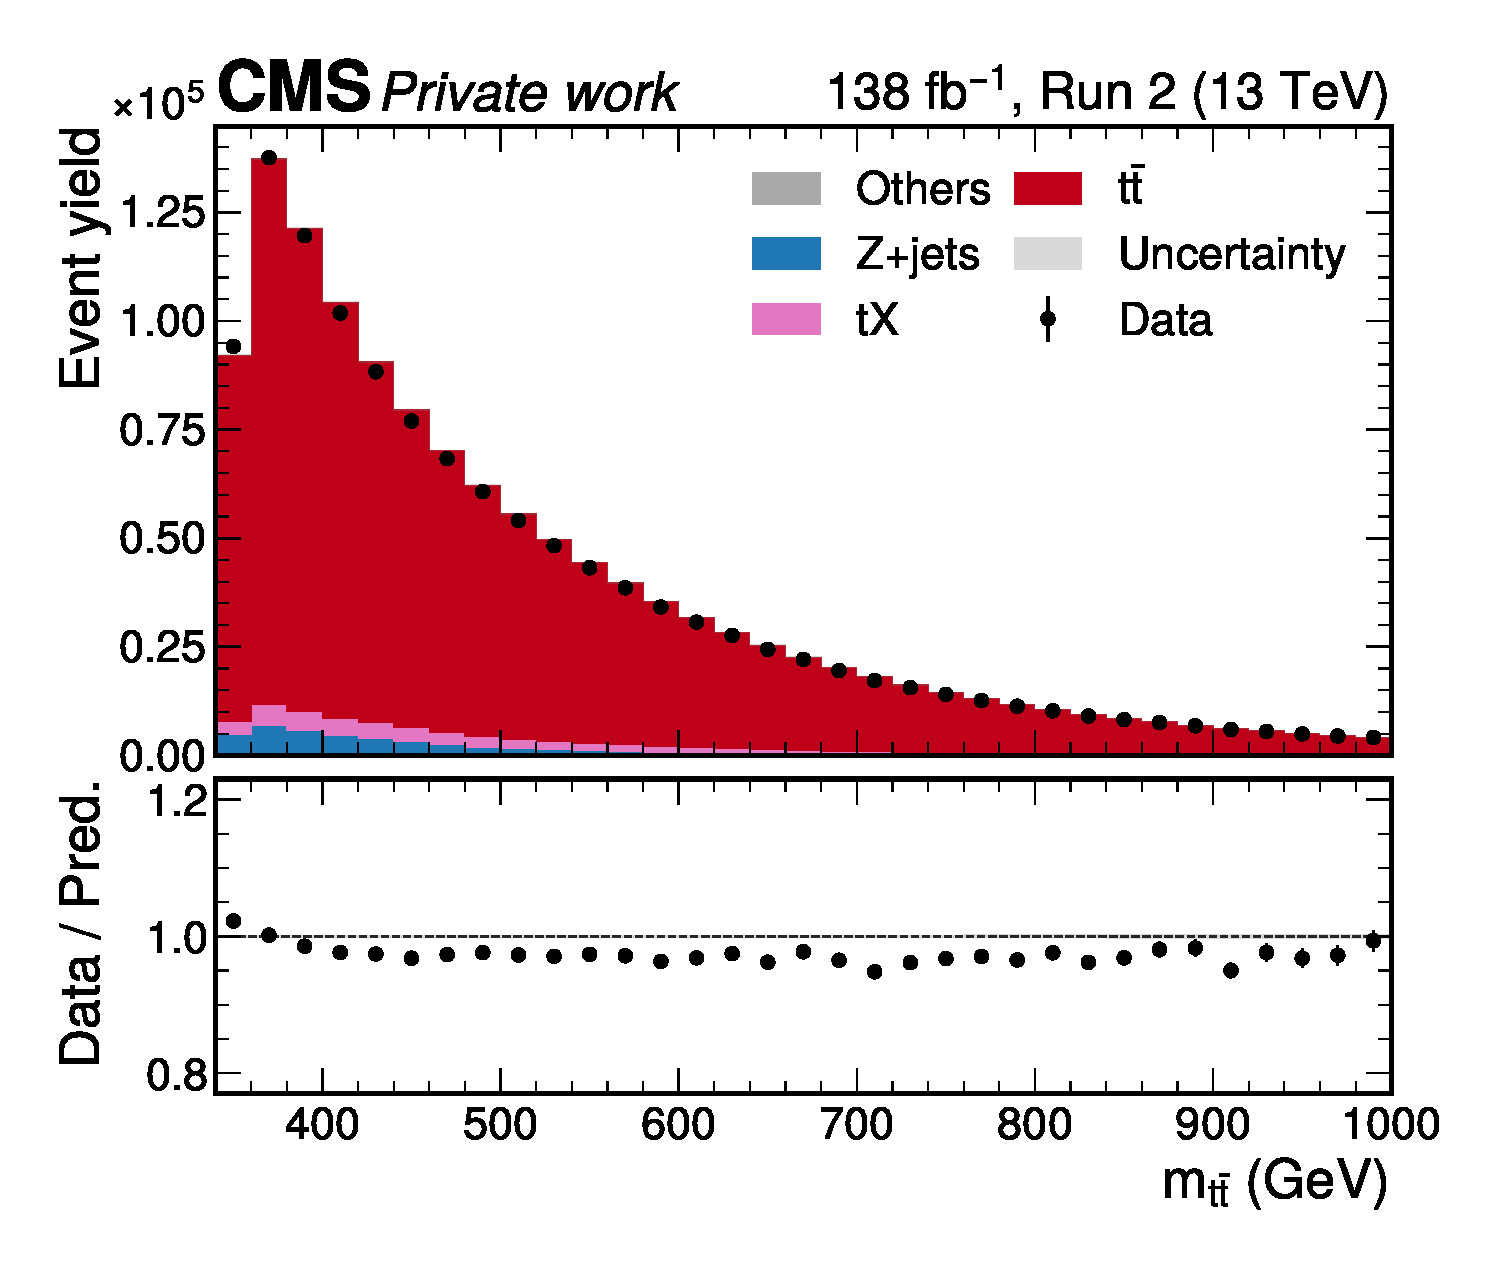
\includegraphics[width=0.49\textwidth]{figures/ah/controlplots/Reco/ll/mtt_Reco_ll.pdf}
    \hfill
    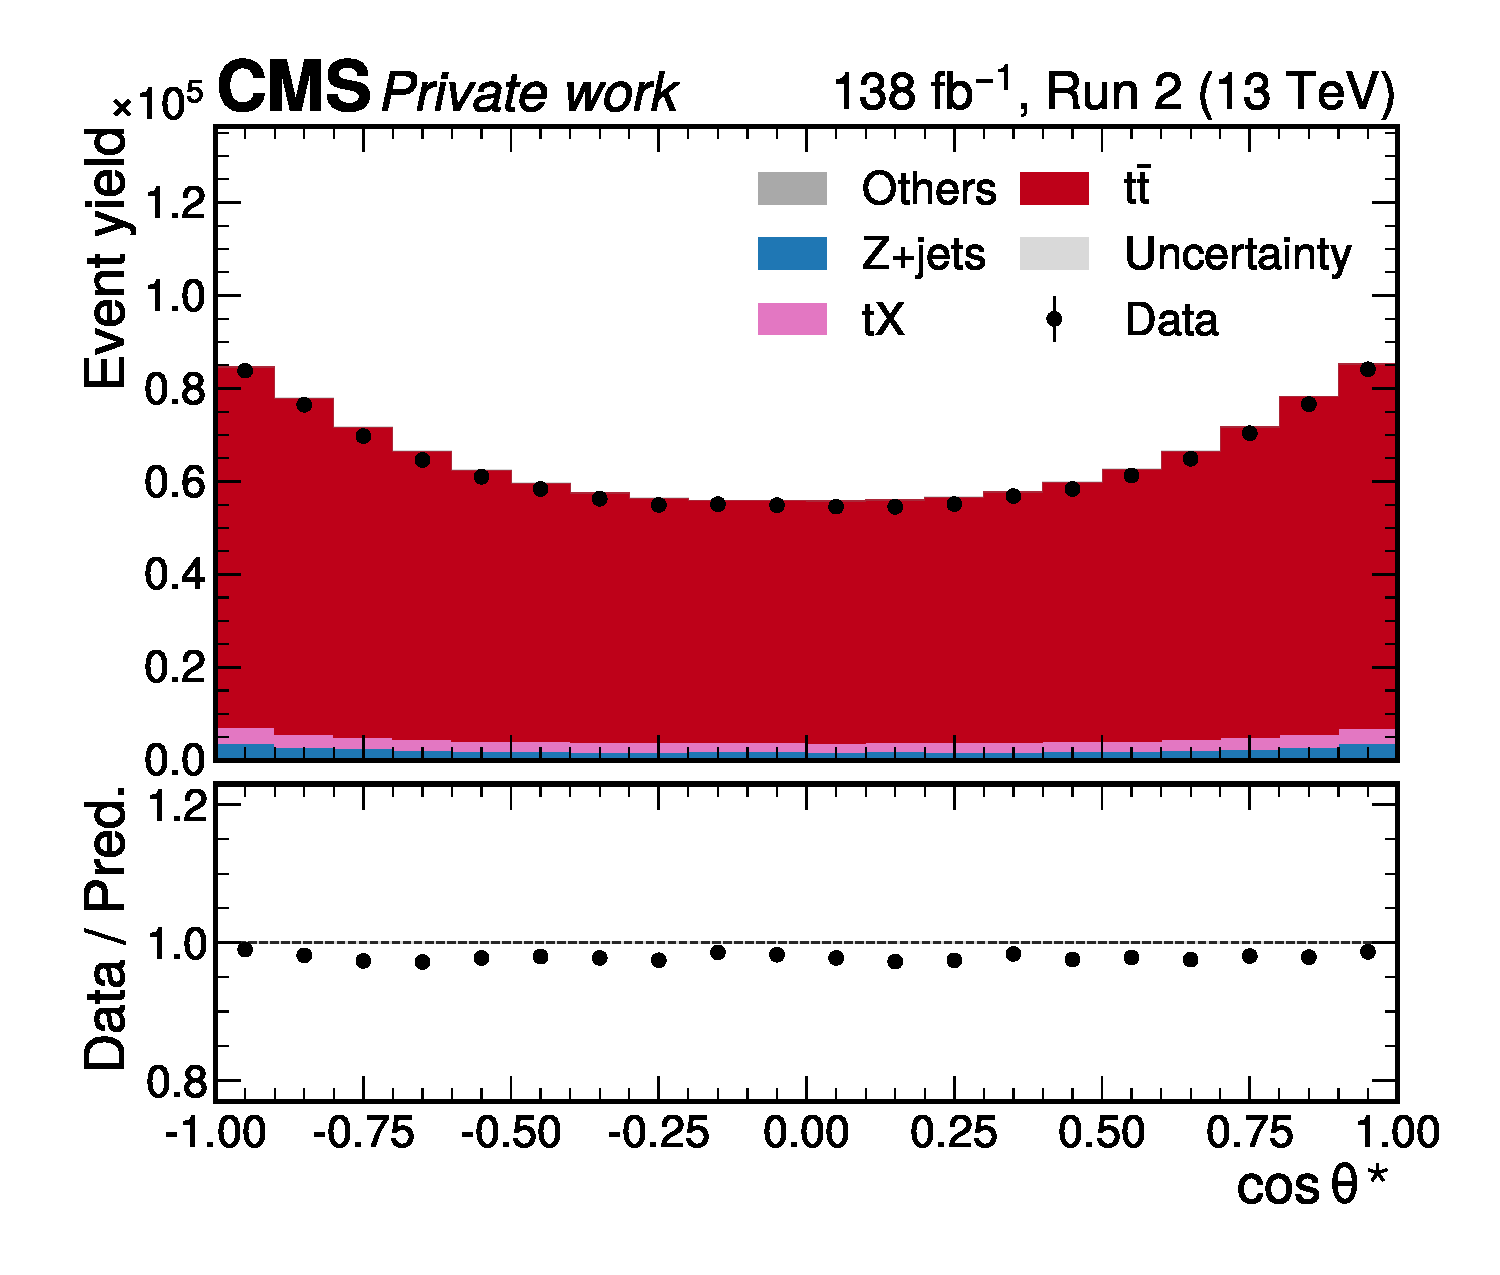
\includegraphics[width=0.49\textwidth]{figures/ah/controlplots/Reco/ll/costhetastar__ll.pdf}
    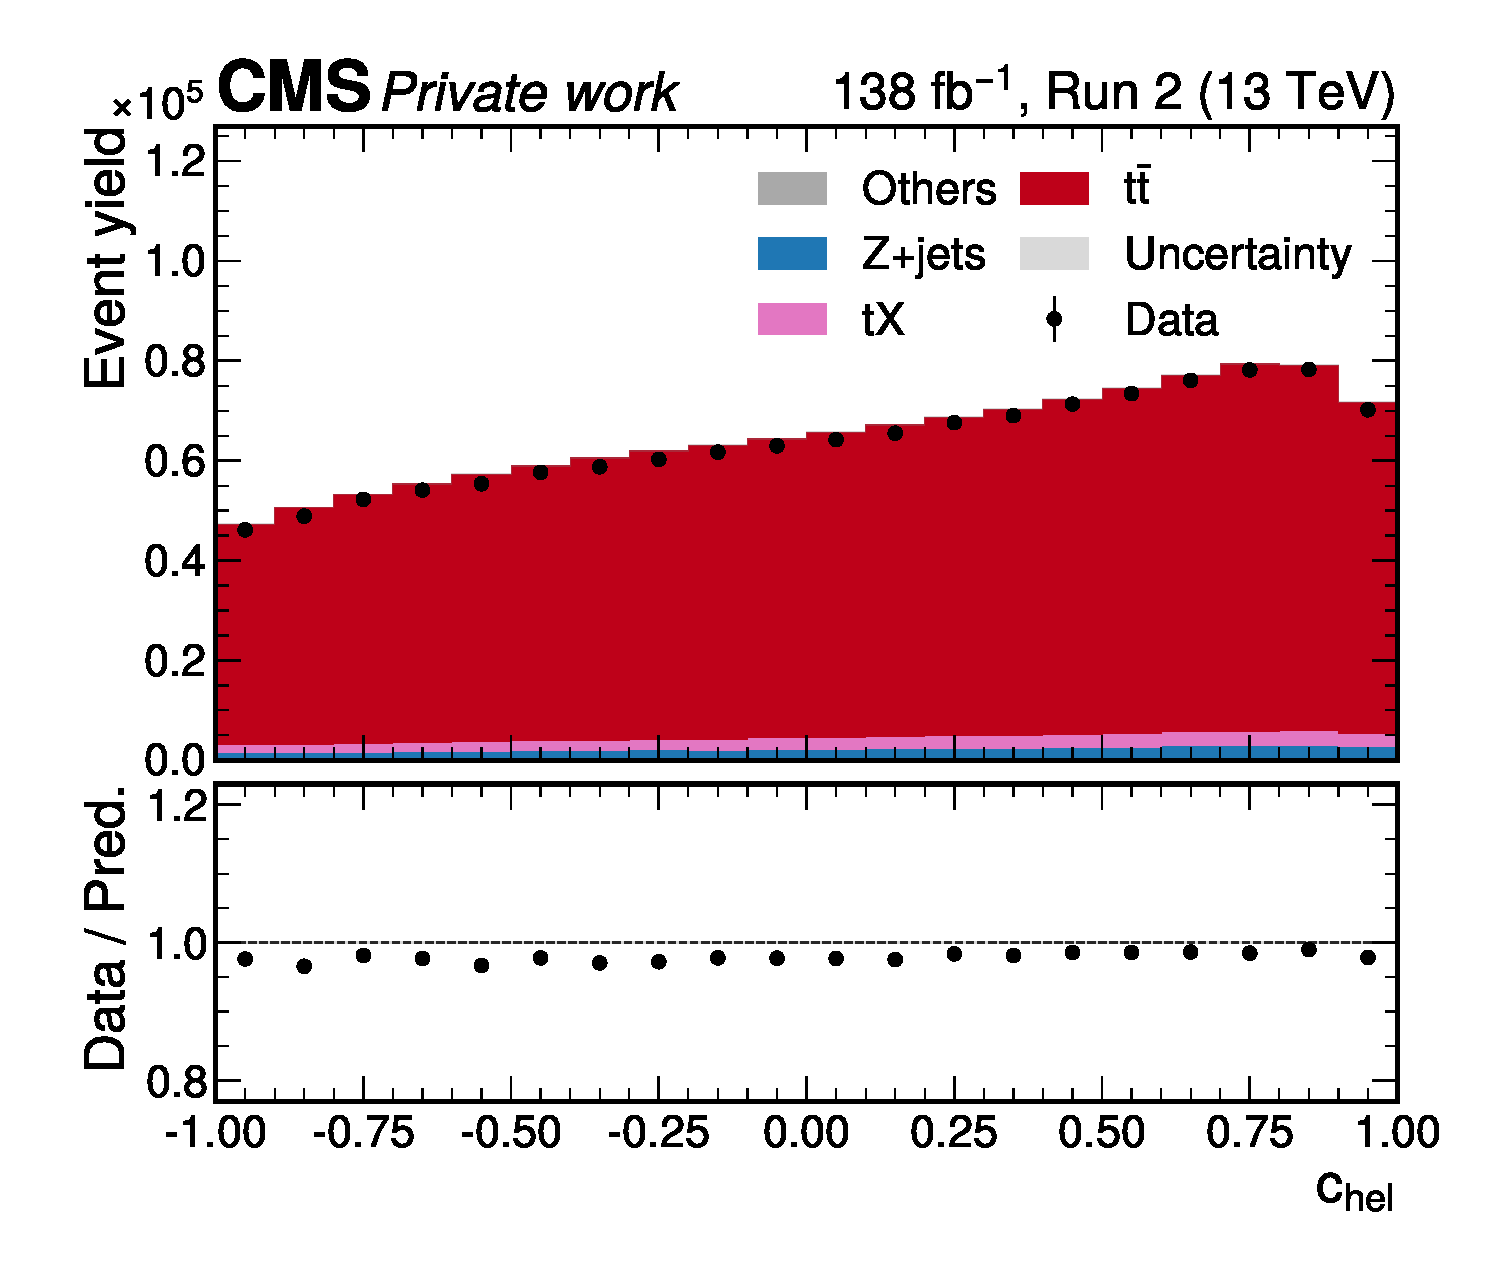
\includegraphics[width=0.49\textwidth]{figures/ah/controlplots/Reco/ll/chel__ll.pdf}
    \hfill
    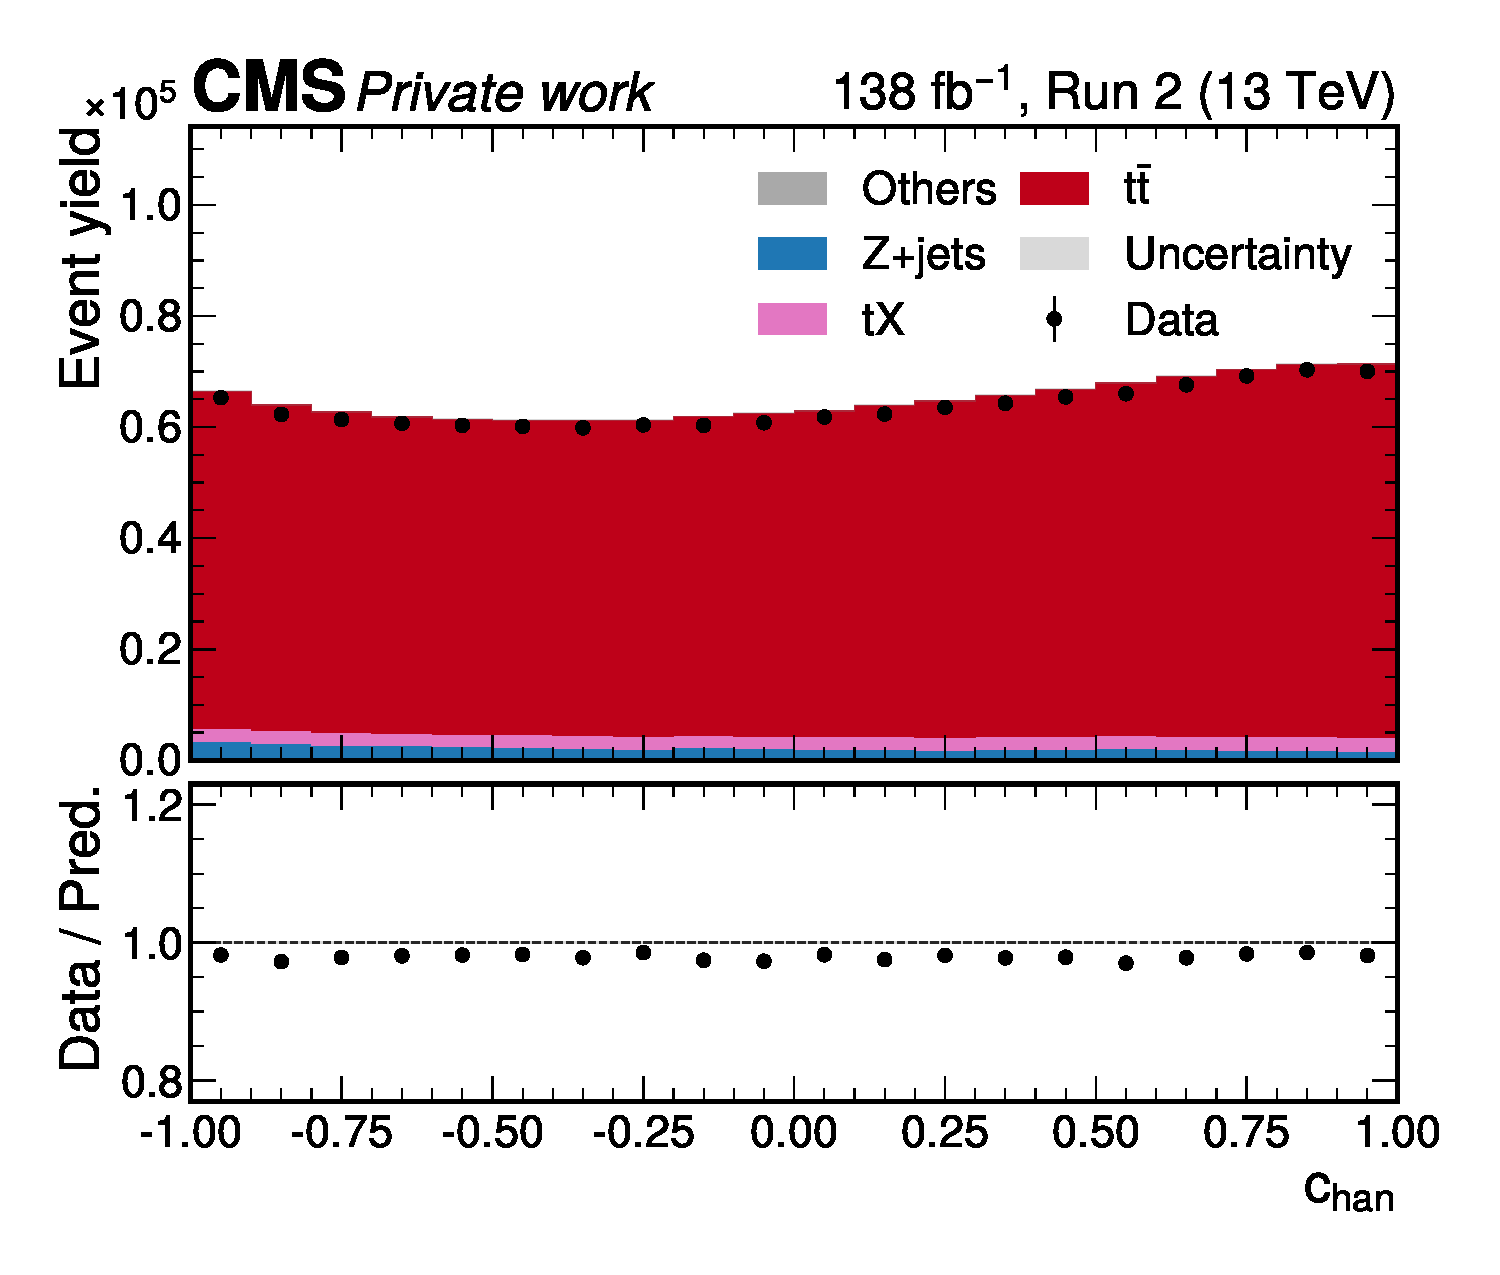
\includegraphics[width=0.49\textwidth]{figures/ah/controlplots/Reco/ll/chan__ll.pdf}
    \caption{
        \textbf{Control distributions after \ttbar reconstruction.} Shown are (from top left to bottom right) the distributions of the top quark \pt, top quark $\eta$, \mtt, \cost, \chel and \chan for the sum of all dilepton channels. All figures show both data (black dots) and different simulated background processes (colored bars), as well as the statistical uncertainty only. 
    }
    \label{fig:ah:controlttbar}
\end{figure}


\section{Extraction of non-perturbative effects in \ttbartitle}
\label{sec:ah:etat}

\section{BSM limits}
\label{sec:ah:limits}

\section{Summary}

